\documentclass[a4paper]{article}

\usepackage{arxiv}

\usepackage[utf8]{inputenc} % allow utf-8 input
\usepackage[T1]{fontenc}    % use 8-bit T1 fonts
\usepackage{hyperref}       % hyperlinks
\usepackage{url}            % simple URL typesetting
\usepackage{booktabs}       % professional-quality tables
\usepackage{amsfonts}       % blackboard math symbols
\usepackage{nicefrac}       % compact symbols for 1/2, etc.
\usepackage{microtype}      % microtypography
\usepackage{multirow}      % microtypography

% Our own Macros
\usepackage{amssymb,amsthm,amsmath}
\usepackage[textsize=small]{todonotes}
\presetkeys{todonotes}{inline}{}

%commentshttps://www.overleaf.com/7481143292gkhcfhbrmxyw
\newcommand{\filip}[1]{\todo[inline, color=green!10]{{\bf Filip:} #1}}
\newcommand{\openprob}[1]{\todo[inline, color=red!10]{{\bf Open problem}: #1}}
\newcommand{\floris}[1]{\todo[inline, color=blue!10]{{\bf Floris:} #1}}

\newcommand{\hash}{\textsc{Hash}}
\providecommand{\st}{}
\renewcommand{\st}{\mathrel{\mid}}
\newcommand{\ldbl}{\{\!\!\{}
\newcommand{\rdbl}{\}\!\!\}}
\newcommand{\Rb}{\mathbb{R}}
\newcommand{\Nb}{\mathbb{N}}
\newcommand{\bF}{\mathbf{F}}
\newcommand{\bB}{\mathbf{B}}
\newcommand{\bC}{\mathbf{C}}
\newcommand{\bW}{\mathbf{W}}
\newcommand{\bN}{\mathbf{N}}
\newcommand{\bA}{\mathbf{A}}
\newcommand{\bJ}{\mathbf{J}}
\newcommand{\labl}{\pmb{\ell}}
\newcommand{\labm}{\pmb{m}}

\newcommand{\architecture}{\mathcal{C}}

\newtheorem{lemma}{Lemma}
\newtheorem{theorem}{Theorem}
\newtheorem{conjecture}{Conjecture}
\newtheorem{proposition}{Proposition}
\newtheorem{definition}{Definition}
\newtheorem{corollary}{Corollary}
\newtheorem{example}{Example}

\title{Loosely Stated, Formally Proved: Kipf and Wellington's GCNs
are Almost 1WL Powerful}

\author{
  Floris Geerts\\
  University of Antwerp\\
  \texttt{floris.geerts@uantwerpen.be}
  \And
  Filip Mazowiecki\\
  Max Planck Institute for Software Sciences\\
  \texttt{filipm@mpi-sws.org}
  \And
  Guillermo A. P\'erez\\
  University of Antwerp\\
  \texttt{guillermoalberto.perez@uantwerpen.be}
  \And
  Adri\'an Soto\\
  Pontificia Universidad Cat\'olica de Chile\\
  \texttt{assoto@uc.cl}
}

\begin{document}

\maketitle

\begin{abstract}
  We adapt ideas from~\cite{grohewl} on the equivalent power of graph neural
  networks and the Weisfeiler-Lehman algorithm.  Then, we leverage the latter
  to provide a rigurous proof that Kipf and Welling's graph convolutional
  networks are indeed Weisfeiler-Leman powerful (and not just loosely speaking
  so).
\end{abstract}

%!TEX root =main.tex
\section{Introduction}\label{sec:intro}
A standard approach to learning tasks on graph structured data, such as vertex classification, edge prediction, and  graph classification, consists of the construction of a \textit{representation} of vertices and graphs that capture their structural information. Graph Neural Networks (GNNs) are currently considered as the state-of-the art approach for learning such representations. Many variants of GNNs exist but they all follow a similar strategy. More specifically,  each vertex is initially associated with a feature vector. This is followed by a recursive neighbourhood aggregation scheme where each vertex aggregates feature vectors of its neighbours, possibly combines this with its own current feature vector, to finally obtain its new feature vector. After a number of iterations, each vertex is then represented by the resulting feature vector. A representation of a graph is  obtained by combining the feature vectors of each of the vertices in some or other way. The latter process is also called pooling. 

The adequacy of GNNs for graph learning tasks is therefore directly related to their so-called \textit{distinguishing power}. Here, distinguishing power refers to the ability of GNNs to distinguish vertices and graphs in terms of their corresponding representations. That is, when two vertices are represented by the same feature vector, they are considered the same with regards to any subsequent feature-based task. Similarly for when two graphs have the same representation.

Only recently a formal study of the distinguishing power of some GNN variants has been initiated. In two independent studies~\cite{xhlj19,grohewl}, it was shown that the distinguishing power of a general class ${\cal C}$ of GNNs is \textit{bounded}. More specifically, in those works, it is shown that for GNNs in ${\cal C}$, two vertices will have the same representation (feature vector) whenever the classical Weisfeiler-Lehman (WL) vertex-colouring algorithm assigns the same colour to these vertices. To recall, the WL algorithm starts from an initial vertex colouring of the graph. Then, similarly as GNNs, the WL algorithm recursively aggregates the colouring of neighbouring vertices. In each recursive step, a vertex colouring is obtained that refines the previous one. The WL algorithm stops when no further refinement is obtained. One then says that the WL algorithm reached the stable vertex colouring. When it comes to distinguishing  graphs, this implies that GNNs in ${\cal C}$ have the same distinguishing power as the WL graph-isomorphism test. This test identifies two graphs whenever they have the same stable vertex colouring. 
In those works, it was further shown that the WL algorithm can be simulated by means of GNNs in ${\cal C}$. As a consequence, the distinguishing power of the class ${\cal C}$ of GNNs agrees with the distinguishing power of the WL algorithm (on vertices) and the WL-test (on graphs).

In this paper we continue the study of the distinguishing power of classes of GNNs that fall outside the class ${\cal C}$ considered in~\cite{grohewl,xhlj19}.  Prominent examples of such GNNs are the so-called Graph Convolutional Networks (GCNs)~\cite{kipf-loose}. Although GCNs adhere to the same strategy as GNNs (i.e., recursive neighbourhood aggregation), they additionally take into account \textit{vertex degree information}. This brings them outside the class ${\cal C}$ of GNNs.  Our main observation is that the distinguishing power of such GCNs is still bounded by the WL algorithm, \textit{but that they are one step ahead}. Intuitively, this is due to the fact that the degree information, which is part of GCNs from the start, is only derived by the WL algorithm after one step. This advantage of GCNs over more classical GNNs may explain the success of GCNs in various graph learning tasks. 

In addition, we show that the WL algorithm \textit{cannot} be simulated by GCNs. This is somewhat contradictory to the general belief that GCNs can be seen as a ``continuous generalisation'' of the WL algorithm. The reason is that the GCNs in~\cite{kipf-loose} assign equal importance between features
of the vertex itself and the features of its neighbours. We show that, by introducing a trade-off parameter between features of the vertex and those of its neighbours, the simulation of the WL algorithm can be achieved. We remark that the incorporation of such a trade-off parameter was already suggested in~\cite{kipf-loose} based on empirical results.
Our simulation result thus provides a theoretical justification of this parameter. We further remark that the trade-off parameter is crucial in the GNN formalism underlying PiNet~\cite{DBLP:journals/corr/abs-1905-03046}.

In the literature one also finds classes of GNNs in which the features of the vertex itself are not taken into account during the recursive aggregation scheme. Since the WL algorithm takes the self-colours into account, it is easily verified that such GNNs have a weaker distinguishing power than those who also use the features of the vertices themselves. Indeed, we show that their distinguishing power is limited by a \textit{weak version of the WL algorithm} (WWL) in which self-colours are ignored. We again show that the WWL algorithm can be simulated by these classes of GNNs.\todo{G: Is this important? Grohe sort of does this but to make it seem important he focuses on unlabelled graphs, right?} 

Finally, in proving our results we refine some of the tools presented in~\cite{grohewl}. In particular, the simulation result of the WL-algorithm depends on the chosen activation function. In~\cite{grohewl}, the sign and ReLU functions were considered. The simulation of the WL algorithm by GNNs using the ReLU activation function was shown by leveraging their simulation of the WL algorithm by GNNs using the sign function. This, however, induces a doubling of the number of layers. We provide a direct simulation of the WL algorithm by GNNs using the ReLU activation function, hereby avoiding the doubling of layers.
Furthermore, as part of our simulation proof we obtain a very simple form of GNNs that only needs a linear number of parameters (linear in the number of vertices in the graph). By contrast, standard GNNs require a quadratic number of parameters in each layer. These simple forms of GNNs may be of independent interest.
\todo{G: up to here it reads quite nice!}

\paragraph{Related work.}
We refer to~\cite{Zhou2018,Zonghan2019} for recent surveys on GNNs and GCNs and instead focus on related work on the distinguishing power of graph neural networks and its connections to the WL-algorithm. As already mentioned,~\cite{xhlj19} and~\cite{grohewl}
were the first to formally establish this connection. Earlier, the WL algorithm already served as inspiration for the design of WL-kernels~\cite{Shrvashidze2011} and the GraphSAGE GNN framework~\cite{Hamilton2017a}. 

The distinguishing power of the WL algorithm itself is well understood
\cite{CaiFI92,KieferSS15,ArvindKRV17}. Connections with logic (chileans).

The work by~\cite{grohewl} in which vertex-labelled undirected graphs were considered has been extended to directed graphs, possibly with vertex- and edge-labels~\cite{Jaume2019}. They show that the distinguishing power is still limited by the corresponding notion of the WL algorithm (see e.g.,~\cite{}). 

About $k$-WL -> morris, also
\cite{NIPS2019_8488} for something in between.

\cite{Wu2019}\cite{Cai2018}: removing activation functions...
\cite{journals/pieee/OrtegaFKMV18} mentions that SGN are equivalent to symmetric normalised Laplacian in~\cite{Vignac2019OnTC} (they also use the inverse of a matrix as propagation schema. Check)

\cite{chen2019powerful}: interesting: they add features $d, Ad, A^2d,\ldots, A^kd$
(simplified iterated degrees). We basically show that GCNs are like GNN that start from ell1, the 1-step WL labelling. This paper seems to do something similar, but slightly more general. They say that it may reduce the number of layers, which would not come as a surprise since you compute some of the WL stuff up-front.

 We should be able to bound this as well. Also, it may even make more sense to replace this with iterated degrees,...

\cite{atamna2019principled}: This seems rubbish, check.

\cite{Hoang2019RevisitingGN} relationship to filters.

\cite{Grel2019AnAO} Spectral and information preservation stuff. Interesting, not sure how it links to expressive power.
Check also Stability and generalization of graph convolutional neural networks

Other kinds of expressiveness questions...check all citations to grohe and xu paper?

\cite{DBLP:journals/corr/abs-1901-09342} universality aspects... check references therein.

position aware GNNs, attention? pooling?
% \cite{Jin2017,Lei2017}
\floris{todo.}

%!TEX root =main.tex
\section{Preliminaries}
\floris{This section may need updating when we finish the rest.
Some notations, like $A_{v\bullet}$ etc are missing. So, we check at the end.}
Let $G=(V,E)$ be an undirected graph consisting of $n$ vertices.
Given a vertex $v\in V$, we denote by $N_G(v)$ its set of neighbors, i.e., $N_G(v):=\{u\st \{u,v\}\in E\}$. Furthermore, the degree of a vertex $v$, denoted by $d_{v}$, is the number of vertices in $N_G(v)$. With a labeled graph $(G,\pmb{\ell})$ we mean a graph $G=(V,E)$ whose vertices are labeled using a function $\pmb{\ell}:V\to \Sigma$
for some set $\Sigma$ of labels.

Given $G=(V,E)$, we denote by $\mathbf{A}$ its adjacency matrix of dimension $n \times n$ such that the entry $\mathbf{A}_{vw}=1$ if $\{v,w\}\in E$ and  $\mathbf{A}_{vw}=0$ otherwise. We denote by $\mathbf{D}$ the diagonal matrix such that $\mathbf{D}_{vv}=d_v$ for each $v\in V$. Throughout the paper we will assume that $G$ does not have isolated nodes, which is equivalent to assuming that $\mathbf{D}$ does not have any $0$ entries on the diagonal. We will also assume that there are no self loops, so the diagonal of $\mathbf{A}$ is filled with $0$s.

Given a labeled graph $(G,\pmb{\ell})$, it will be convenient to regard the vertex labeling $\pmb{\ell}$ as a vector in $\Rb^{n\times 1}$ such that $\pmb{\ell}_v:=\pmb{\ell}(v)$. Here, without loss of generality, we silently assume an embedding of  the set $\Sigma$ of labels in $\Rb$. More generally, we also consider vertex labelings in which 
vertices in $G$ are labeled  with vectors from $\Rb^q$, for some dimension $q \in \Nb$. 
Given a matrix $\mathbf{F} \in \Rb^{n \times q}$, we refer to the vertex labeling (induced by)
$\mathbf{F}$ as the labeling which associates vertex $v$ with label the row vector  $\mathbf{F}_{v\bullet}$.

It will be important later on to be able to compare two labelings of $G$.
Given a matrix $\mathbf{F} \in \Rb^{n\times q}$ and a matrix $\mathbf{F}' \in \Rb^{n\times q'}$ we say that the
vertex labeling  $\mathbf{F}'$ is coarser than the vertex labeling $\mathbf{F}$, denoted by $\mathbf{F}\sqsubseteq \mathbf{F}'$, if
for all $v,w\in V$,
$
\mathbf{F}_{v\bullet}=\mathbf{F}_{w\bullet} \Rightarrow \mathbf{F}'_{v\bullet}=\mathbf{F}'_{w\bullet}
$
The vertex labelings $\mathbf{F}$ and $\mathbf{F}'$ are equivalent, denoted by $\mathbf{F}\equiv\mathbf{F}'$, if $\mathbf{F}\sqsubseteq \mathbf{F}'$ and
$\mathbf{F}'\sqsubseteq \mathbf{F}$ hold. In other words, $\mathbf{F}\equiv\mathbf{F}'$ if and only if for all $v,w\in V$,
$
\mathbf{F}_{v\bullet}=\mathbf{F}_{w\bullet} \Leftrightarrow \mathbf{F}'_{v\bullet}=\mathbf{F}'_{w\bullet}
$.

Of particular importance is the labeling obtained by color refinement, also known as Weisfeiler-Lehman (or WL, for short). The WL procedure constructs a labeling, in an incremental fashion, based on neighborhood information. More specifically, consider a labeled graph $(G,\pmb{\ell})$. Initially, 
$\pmb{\ell}^{(0)}:=\pmb{\ell}$. Then, the WL procedure computes a labeling $\pmb{\ell}^{(t)}$, for $t> 0$, as follows: 
$$
\pmb{\ell}^{(t)}_v:=\textsc{Hash}\Bigl(\bigl(\pmb{\ell}^{(t-1)}_v,\ldbl \pmb{\ell}_u^{(t-1)} \st u \in N_G(v) \rdbl\bigr)\Bigr),
$$
where $\textsc{Hash}$ bijectively maps the above pair, consisting of (i)~the previous label 
$\pmb{\ell}^{(t-1)}_v$ of $v$; and (ii)~the multi-set $\ldbl \pmb{\ell}_u^{(t-1)} \st u \in N_G(v) \rdbl$ of labels of $v$'s neighbors, to a unique label in $\Sigma$, which has not been used in previous iterations. When the number of distinct labels in $\pmb{\ell}^{(t)}$ and $\pmb{\ell}^{(t-1)}$ is the same, the 1-WL algorithm terminates.
Termination is guaranteed in at most $n$ steps. We refer to the resulting labeling as the \textit{WL labeling of $(G,\pmb{\ell})$}. 
%!TEX root =main.tex


\section{Graph neural networks}
Neural networks are a model to compute functions $f : \Rb^s \to \Rb^k$ obtained as a composition of layers $l^1,\ldots, l^m$. Every layer $l^t$ computes a function $f^{(t)} : \Rb^{k_{t-1}} \to \Rb^{k_t}$ based on the previous layer, where $k_0 = s$ and $k_m =k$. Formally, every layer $l^t$ is given by
\begin{equation}\label{eq:NN}
 l^t(f^{(t-1)}) = \sigma \left(\bW^{(t)} \vec{x} + b^{(t)}  \right),
\end{equation}
where: $\bW^{(t)} \in \Rb^{k_{t} \times k_{t-1}}$ is called the \emph{weight}; $b^{(t)} \in \Rb^{k_t}$ is called the \emph{bias}; and $\sigma$ is an \emph{activation function}. Activation functions are nonlinear transformations that are applied pointwise. We will discuss them in more detail later. We will consider several architectures of neural networks that are defined as variants of~\eqref{eq:NN}.
% The most common example is ReLU defined as $\max(\cdot, 0)$ on every point.

In this paper we are interested in architectures of \emph{graph neural networks} (GNN in short).
There are many different architectures for GNNs in the literature. The goal of this paper is to compare these architectures in terms of expressiveness, therefore we start by giving a very general definition of a GNN. Afterwards, we will discuss how particular architectures are captured by this definition.

A GNN is defined with respect to a labelled graph $(G,\labl)$, where $G = (V,E)$ and $\labl : V \to \Rb^{k}$. A GNN computes a function $f : L_s \to L_k$, where $L_j$ is the set of all labellings $f : V \to \Rb^j$.
We will identify every labelling $f \in L_j$ with a matrix $F \in \Rb^{n \times j}$ by putting the label of every node in a separate row.
A GNN is obtained as composition of layers that compute labellings $l^1, \ldots, l^m$, where every layer computes $l^t(f^{(t-1)}) = f^{(t)} \in L_{k_t}$ and $f^0 = \labl$. For every $f^{(t)}$ let $\bF^{(t)} \in \Rb^{n \times k_{t}}$ be its corresponding matrix. We consider architectures, where each layer $l^t$ is of the form
\begin{equation}\label{eq:GNN}
l^t(\bF^{(t)}) = \sigma \left( \bN^{(t)}\bF^{(t)}\bW_1^{(t)} + \bF^{(t)}\bW_2^{(t)} + \bB^{(t)} \right),
\end{equation}
where $\bN^{(t)} \in \Rb^{n \times n}$ is called the \emph{neighbourhood}, $\bW_1^{(t)}, \bW_2^{(t)} \in \Rb^{k_{t-1} \times k_t}$ are called \emph{weights}, and $\bB^{(t)} \in \Rb^{n \times k_t}$ is called the \emph{bias}. Compared to~\eqref{eq:NN} the main differences are
\begin{itemize}
 \item that there are two weight matrices and they are on the right side.
 \item
\end{itemize}

More specifically, a GNN computes for each vertex $v\in V$ a feature vector $\mathbf{F}^{(t)}_{v\bullet}$  in layer $t$ by combining:
\begin{itemize}
	\item[] (i)~the feature vector $\mathbf{F}^{(t-1)}_{v\bullet}$ of $v$ from the previous layer; and
	\item[] (ii)~the multi-set of features from the previous layer  of $v$'s neighbors, i.e., the multi-set $\ldbl \mathbf{F}^{(t-1)}_{u\bullet} \st u \in N_G(v) \rdbl$.
\end{itemize}
One typically parametrizes GNNs by how this combination is achieved. We here follow~\cite{grohewl,DBLP:conf/iclr/XuHLJ19}  in which combination and aggregation functions for each layer $t$ are considered, denoted by
$f_{\textsl{comb}}^{(t)}$ and
$f_{\textsl{agg}}^{(t)}$, respectively, and features are updated as follows.  For each vertex $v\in V$ and layer $t$:
\begin{equation}
\mathbf{F}^{(t)}_{v\bullet}:=
f_{\textsl{comb}}^{(t)}\Bigl(
\mathbf{F}_{v\bullet}^{(t-1)},f_{\textsl{aggr}}^{(t)}\bigl(\ldbl \mathbf{F}^{(t-1)}_{u\bullet} \st u \in N_G(v) \rdbl\bigr)
\Bigr), \label{lab:generalGNN}
\end{equation}
 Finally, if a GNN consists of $L$ layers then
$\mathbf{F}^{(L)}$ is used to classify the vertices in $G$ different classes. More precisely, vertices $v$ and $w$ will belong to the same class if and only if 
$\mathbf{F}^{(L)}_{v\bullet}=\mathbf{F}^{(L)}_{w\bullet}$, i.e., when their feature vectors are equal.

The way that GNNs update feature vectors is clearly reminiscent of how the WL procedure works. The relationship between vertex classification by GNNs of the form~(\ref{lab:generalGNN}) and vertex classification by WL can be made precise~\cite{grohewl,DBLP:conf/iclr/XuHLJ19}. To state this relation formally, we define the notions of being \textit{bounded by WL}, for upper bounding the classification power of GNNs, and being \textit{WL-strong}, for lower bounding the classification power of GNNs~\cite{grohewl}. 

\begin{definition}[Bounded by WL]\normalfont\label{def:wlupper}
Let $(G,\pmb{\ell})$ be a labeled graph and let $\pmb{\ell}^{(0)}:=\pmb{\ell}$. Furthermore, denote by 
$\pmb{\ell}^{(t)}$ the vertex labeling obtained after $t$ iterations of the WL procedure, starting from $\pmb{\ell}^{(0)}$. Let $\mathbf{F}^{(t)}$ be feature matrices computed using a GNN of the form ~(\ref{lab:generalGNN}), for $t\geq 0$. Then, given $\mathbf{F}^{(0)}$ such that $\pmb{\ell}^{(0)}\sqsubseteq \mathbf{F}^{(0)}$ holds, one says that the GNN  is \textit{bounded by WL} if for all $t\geq 0$, 
$\pmb{\ell}^{(t)}\sqsubseteq \mathbf{F}^{(t)}$.
% That is, the vertex labeling induced by $\mathbf{F}^{(t)}$ is always coarser than the vertex labeling $\pmb{\ell}^{(t)}$  obtained by WL after $t$ iterations.
\end{definition}
In terms of vertex classification this implies that when a GNN is bounded by WL, then 
for every $t$, when WL classifies two vertices as the same in step $t$, then so does the GNN. 

The boundedness property holds for \textit{any} GNN of the form~(\ref{lab:generalGNN}):
\begin{proposition}[~\cite{grohewl,DBLP:conf/iclr/XuHLJ19}]\label{prop:upperboundgeneral}
% Let $(G,\pmb{\ell})$ be a labeled graph and let $\mathbf{F}^{(0)}$ consist of feature vectors such that $\pmb{\ell}^{(0)}\sqsubseteq \mathbf{F}^{(0)}$. Then, $\pmb{\ell}^{(t)}\sqsubseteq \mathbf{F}^{(t)}$ for every $t>0$, where $\mathbf{F}^{(t)}$ is computed by a
Any GNN of the form~(\ref{lab:generalGNN}) is bounded by WL.
\end{proposition}


When the combination and aggregation functions are assumed to be all injective one can further show that GNNs of the form~(\ref{lab:generalGNN}) are also as powerful as WL~\cite{DBLP:conf/iclr/XuHLJ19}. That is, when two vertices are classified as the same by the GNN then they are also classified the same by WL. 
We can phrase this more generally in terms of \textit{classes} of GNNs. Here, a class of GNNs is simply a collection of GNNs of the form~(\ref{lab:generalGNN}) in which the allowed aggregation and combination functions are restricted to belong to some class. For example, one could consider the class of injective functions for the combination and aggregation functions.

\begin{definition}[WL-strong]\normalfont\label{def:wlstrong}
A \textit{class} of GNNs of the form~(\ref{lab:generalGNN}) is \textit{WL-strong} if for any given labeled graph
	$(G,\pmb{\ell})$, there exist instantiations of the combination and aggregation functions in that class such that for all $t\geq 0$, $\mathbf{F}^{(t)}\sqsubseteq \pmb{\ell}{}^{(t)}$.
\end{definition}

Clearly, for classes of GNNs of the form~(\ref{lab:generalGNN}) that are WL-strong, 
Proposition~\ref{prop:upperboundgeneral} implies that for every labeled graph $(G,\pmb{\ell})$ there
exist instantiations of the combination and aggregation functions in that class such that
for all $t\geq 0$, $\mathbf{F}^{(t)}\equiv \pmb{\ell}{}^{(t)}$. That is, there is at least one particular instantiation of the GNNs in the class that is equivalent to WL in terms of vertex classification.

A specific class of GNNs which is known to be WL-strong~\cite{grohewl} is given by:
\begin{equation}
\mathbf{F}^{(t)}:=\sigma\Bigl(\mathbf{F}^{(t-1)}\mathbf{W}_1^{(t)}+ \mathbf{A}\mathbf{F}^{(t-1)}\mathbf{W}_2^{(t)} + \mathbf{B}^{(t)}\Bigr), \label{eq:groheGNN}
\end{equation}
where $\mathbf{W}_1^{(t)}$, $\mathbf{W}_2^{(t)}$  are weight matrices, $\mathbf{B}^{(t)}$ are 
constant\footnote{A constant matrix is matrix which is a multiple of the all-ones matrix $\mathbf{J}$.} bias matrices, and $\sigma$ is the sign function. It is readily verified that GNNs of the form~(\ref{eq:groheGNN}) can be seen as  GNNs of the form~(\ref{lab:generalGNN}). Hence, GNNs of the form~(\ref{eq:groheGNN}) are also bounded by WL by Proposition~\ref{prop:upperboundgeneral}.

More specifically, it was shown in~\cite{grohewl} that even the class of GNNs of the form
\begin{equation}
\mathbf{F}^{(t)}:=\sigma\Bigl(\mathbf{F}^{(t-1)}\mathbf{W}_1^{(t)}+ \mathbf{A}\mathbf{F}^{(t-1)}\mathbf{W}_2^{(t)} - \mathbf{J}\Bigr), \label{eq:groheGNNwithJ}
\end{equation}
is WL-strong. That is, compared to class of GNNs of the form~(\ref{eq:groheGNN}), the bias matrices $\mathbf{B}^{(t)}$ is now chosen uniformly (for all layers) to be $-\mathbf{J}$.


\openprob{Although the result reported in~\cite{grohewl} is correct, it is not entirely clear how their construction translates into an architecture of the form~\ref{eq:groheGNN}. Their construction fits, however, in an architecture of the
form $\mathbf{F}^{(t)}:=\Bigl(\mathbf{F}^{(0)},\sigma\bigl(\mathbf{F}^{(t-1)}\mathbf{W}_1^{(t)}+ \mathbf{A}\mathbf{F}^{(t-1)}\mathbf{W}_2^{(t)} -\mathbf{J}\bigr)\Bigr)$ which is not exactly in the form of ~\ref{eq:groheGNN}. We will recover the WL-strongness result from ~(\ref{eq:groheGNN}) as a side result of our analysis, however. {\bf BUT: is it true that their update rule cannot be expressed as they claim??}}.
\floris{It seems to be possible after all, provided that a slightly more general bias matrix is used. That is, to show strongness we can consider. Please check. An additional assumption is that $\sigma(\mathbf{F}^{(0)})=\mathbf{F}^{(0)}$.}
$$
[\mathbf{F}^{(0)},\mathbf{F}^{(t)}]:=\sigma\left([\mathbf{F}^{(0)},\mathbf{F}^{(t-1)}]\begin{pmatrix}
\mathbf{I}_{n\times n} & \mathbf{O}_{n\times n}\\
\mathbf{O}_{n\times n} & \mathbf{O}_{n\times n}\end{pmatrix}
+\mathbf{A}[\mathbf{F}^{(0)},\mathbf{F}^{(t-1)}]
\begin{pmatrix}
\mathbf{O}_{n\times n} & \mathbf{O}_{n\times n}\\
\mathbf{O}_{n\times n} & \mathbf{W}_{n\times n}^{(t-1)}\end{pmatrix}-
q\begin{pmatrix}
\mathbf{O}_{n\times n} & \mathbf{J}_{n\times n}\\
\mathbf{O}_{n\times n} & \mathbf{J}_{n\times n}\end{pmatrix}
\right),
$$
where $\mathbf{W}^{(t-1)}$ is the matrix constructed in Grohe's lower bound proof.
\floris{Our lower bound shows that it holds also for a simpler GNN architecture, however,
see below, and also we can deal with ReLU.}

In~\cite{grohewl}, also GNNs of the form~\ref{eq:groheGNNwithJ} where considered in which the activation function $\sigma$ is the ReLU function. In this case, the relationship
$\mathbf{F}^{(2t)}\sqsubseteq \pmb{\ell}^{(t)}$ holds, for every $t\geq 0$~\cite{grohewl}.
Strictly speaking this architecture is not WL strong in the sense of Definition~\ref{def:wlstrong}. Later in the paper we show that the factor two can be avoided, however, by allowing a bias matrix of the form $-q\mathbf{J}$ for some parameter $q$.
In fact, we establish WL-strongness for
an even more restricted class of GNNs of the form:
\begin{align}
\mathbf{F}^{(t)}&:=\sigma\Bigl(p\mathbf{F}^{(t-1)}\mathbf{W}^{(t)}+ \mathbf{A}\mathbf{F}^{(t-1)}\mathbf{W}^{(t)} - q\mathbf{J}\Bigr), \label{eq:GNN}\\
&:=\sigma\Bigl((\mathbf{A}+p\mathbf{I})\mathbf{F}^{(t-1)}\mathbf{W}^{(t)} - q\mathbf{J}\Bigr), \label{eq:GNN2}
\end{align}
for parameters $p, q$ such that $0< p,q<1$ is WL-strong, where $\sigma$ is either the sign or ReLU activation function. Here, $\mathbf{I}$ is the identity matrix of appropriate dimension.
Compared to~(\ref{eq:groheGNNwithJ}) we only have one weight matrix $\mathbf{W}^{(t)}$ in each layer and have two additional parameters $p$ and $q$\footnote{A technical condition for obtaining WL-strongness is that  the initial feature matrix $\mathbf{F}^{(0)}$ satisfies $\mathbf{F}^{(t)}\equiv \pmb{\ell}^{(0)}$  and that
the unique rows in $\mathbf{F}^{(0)}$ are linearly independent. It will become clear later why this assumption is needed.}



%
% \todo{I believe that this lower bound indeed holds, but the proof given in ~\cite{grohewl} is not correct. I do not see how their approach for the labeled case can be squeezed in the above form. I emailed Martin about this (I keep you in the loop when I get some response.). Why does it hold, because we show later that
% $$
% \mathbf{F}^{(t)}:=\sigma\Bigl((\mathbf{A}+p\mathbf{I})\mathbf{F}^{(t-1)}\mathbf{W}_2^{(t)} +\mathbf{W}_3^{(t)}\Bigr),
% $$
% is WL-strong for $p<1$, which is an instance of that more general architecture.
% }

% \todo{Argue that the normalized adjacency and augmented adjacency (Kipf) do not fit in this framework, whereas the others do but are not WL strong. This motivates to look at a small unifying architecture and study its expressive power.
% }
% A graph neural network (GNN) model consists of layers, where each layer specifies how to update a vertex labeling $\mathbf{F}$. A GNN with $k$ layers is defined by updates of $\mathbf{F}^{(t)}$ for $t = 0, \ldots,k$, which denotes the labeling obtained after $t$ layers. A new labeling $\mathbf{F}^{(t+1)}$ is obtained inductively by transformations defined on the previous labeling $\mathbf{F}^{(t)}$. An \emph{architecture} specifies what kind of transformations are allowed.


Although GNN architectures of the form~(\ref{eq:groheGNN}) or~(\ref{eq:GNN}) are quite general,  they do not capture some common GNN architectures used in the literature:
%
\floris{We may want to add references to the architectures below. This requires some googling around. Also, not entirely happy with the acronym's.
Better suggestions are welcome!}
% Well-known GNN architectures can be obtained from~(\ref{eq:architecture}) by varying $\mathbf{L}$ and $\mathbf{R}$, $p$ and $q$, as follows:
\begin{description}
% \item[\textit{Adjacency}:]
% % $\mathbf{L}=\mathbf{R}:=\mathbf{I}$, $p=q:=0$. Hence,
% $
% \mathbf{F}^{(t+1)}:=\sigma\left(\mathbf{A}\mathbf{F}^{(t)}\mathbf{W}^{(t)}\right)
% $
\item[\textit{Random walk (RW-GNN)}:] 
% $\mathbf{L}:=\mathbf{D}^{-1}$ with $\mathbf{D}$ the degree matrix of $\mathbf{A}$, $\mathbf{R}:=\mathbf{I}$, $p=q:=0$. Hence,
$$
\mathbf{F}^{(t)}:=\sigma\left(\mathbf{D}^{-1}\mathbf{A}\mathbf{F}^{(t-1)}\mathbf{W}^{(t-1)}\right);$$
\item[\textit{Normalized adjacency (NA-GNN)}:] 
% $\mathbf{L}=\mathbf{R}:=\mathbf{D}^{-1/2}$, $p=q:=0$. Hence,
$$
\mathbf{F}^{(t)}:=\sigma\left(\mathbf{D}^{-1/2}\mathbf{A}\mathbf{D}^{-1/2}\mathbf{F}^{(t-1)}\mathbf{W}^{(t-1)}\right)
;$$
\item[\textit{$1$st Order GCN (1-GCN)}:]
$$
\mathbf{F}^{(t)}:=\sigma\left(\mathbf{F}^{(t-1)}\mathbf{W}_1^{(t-1)}+\mathbf{D}^{-1/2}\mathbf{A}\mathbf{D}^{-1/2}\mathbf{F}^{(t-1)}\mathbf{W}_2^{(t-1)}\right);$$

\item[\textit{Simplified $1$st Order GCN (1-GCNs)}:]
$$
\mathbf{F}^{(t)}:=\sigma\left((\mathbf{D}^{-1/2}\mathbf{A}\mathbf{D}^{-1/2}+\mathbf{I})\mathbf{F}^{(t-1)}\mathbf{W}_2^{(t-1)}\right);$$
\item[\textit{Augmented random walk (RW-GNN+)}:] 
% $\mathbf{L}:=\tilde{\mathbf{D}}^{-1}$ with $\tilde{\mathbf{D}}$ the degree matrix of $\mathbf{A}+\mathbf{I}$, $\mathbf{R}:=\mathbf{I}$, $p:=1$, $q:=0$. Hence,
$$
\mathbf{F}^{(t)}:=\sigma\left(\tilde{\mathbf{D}}^{-1}(\mathbf{A}+\mathbf{I})\mathbf{F}^{(t-1)}\mathbf{W}^{(t-1)}\right),$$
with $\tilde{\mathbf{D}}$ the degree matrix of $\mathbf{A}+\mathbf{I}$; and
\item[\textit{Augmented adjacency (NA-GNN+)}~\cite{kipf-loose}:] % $\mathbf{L}=\mathbf{R}:=\tilde{\mathbf{D}}^{-1/2}$, $p:=1$, $q:=0$. Hence,
$$
\mathbf{F}^{(t)}:=\sigma\left(\tilde{\mathbf{D}}^{-1/2}(\mathbf{A}+\mathbf{I})\tilde{\mathbf{D}}^{-1/2}\mathbf{F}^{(t-1)}\mathbf{W}^{(t-1)}\right);
$$
\item[\textit{Weighted augmented adjacency (NA-GNN++)}~\cite{DBLP:journals/corr/abs-1905-03046}:]
$$\mathbf{F}^{(t)}:=\sigma\left((r\mathbf{I}+(1-r)\tilde{\mathbf{D}})^{-1/2}(\mathbf{A}+p\mathbf{I})(r\mathbf{I}+(1-r)\mathbf{D})^{-1/2}\mathbf{F}^{(t-1)}\mathbf{W}^{(t-1)}\right),
$$
which underlies the PiNet architecture.
\end{description}
% Bias can be added to all previous architectures by setting $q\neq 0$.
This begs the question how these architectures relate to WL. This question is of particular importance for the augmented adjacency architecture which is often regarded as a continuous version of WL~\cite{kipf-loose}
\floris{We may want to sell the connection with Kipf a bit more, especially as it served as our motivation to look in all. this.}
Indeed, it is mentioned in ~\cite{kipf-loose} that the augmented adjacency architecture can be interpreted -- loosely speaking -- as differentiable and parameterized WL process on graphs. This claim has, to our knowledge, not been made formal.


% \todo{I believe that we separate these architectures based on:
% \begin{itemize}
% 	\item Presence/absence of $\mathbf{I}$: This relates to labeled vs unlabeled graphs.
% 	\item Presence/absence of $\mathbf{R}$: This relates to being one-step ahead compared to WL.
% 	\item Presence/absence of $\mathbf{L}$: ??
% 	\item parameter $p<1$: this is crucial for being WL-strong.
% \end{itemize}}
To analyze the expressive power of all these GNN architectures we therefore consider a general GNN architecture of the form:
% We consider a GNN architecture which generalises commonly used GNN architectures. Given a labeled
% graph $(G,\pmb{\ell})$ with $G=(V,E)$, we denote by $\mathbf{F}^{(t)}$ the feature matrix assigning to each vertex $v\in V$ a feature vector $\mathbf{F}_{v\bullet}$. In layer $t$ of the the GNN architecture, $\mathbf{F}^{(t)}$ is updated as follows:
\begin{equation}
\mathbf{F}^{(t)}:=\sigma\left(\mathbf{F}^{(t-1)}\mathbf{W}_1^{(t-1)}+\mathbf{L}(\mathbf{A}+p\mathbf{I})\mathbf{R}\mathbf{F}^{(t-1)}\mathbf{W}_2^{(t-1)} + q\mathbf{J}\right), \label{eq:architecture}
\end{equation}
where $\mathbf{L}$ and $\mathbf{R}$ positive diagonal matrices, $p$ and $q$ are  learnable parameters in $[0,1]$, and $\mathbf{W}_1^{(t-1)}$ and $\mathbf{W}_2^{(t-1)}$  are learnable weight matrices, and finally, $\sigma$ is a non-linear activation function such as sign or ReLU. It should be clear that by choosing 
$\mathbf{L}$, $\mathbf{R}$, $p$ and $q$  in an appropriate way, one can obtain all  GNN architectures mentioned so far.

In the remainder of the paper we investigate the expressive power of GNNs of the form~(\ref{eq:architecture}) in detail. We remark that our proof techniques are similar to those used in~\cite{grohewl} but with some minor twists.

% above. Furthermore, we see that~(\ref{eq:architecture}) also encompasses the architecture~(\ref{eq:GNN2}).
% Our analysis also works for the even more general setting
% \begin{equation}
% \mathbf{F}^{(t+1)}:=\sigma\left(\mathbf{F}^{(t)}\mathbf{W_1}+\mathbf{L}(\mathbf{A}+p\mathbf{I})\mathbf{R}\mathbf{F}^{(t)}\mathbf{W}_2^{(t)} + \mathbf{W_3}\right), \label{eq:architecture}
% \end{equation}
% \todo{Perhaps we should use this general version. It does not make a difference of the upper bound, and we do not need $\mathbf{F}^{(t)}\mathbf{W_1}$ to show it is WL strong in our modified sense.}

% \section{Expressive Power}
% It is common to measure the expressive power of GNN architectures in comparison with the 1-WL algorithm~\cite{grohewl,DBLP:conf/iclr/2019}.  Complementary, if for \textit{any} given labeled graph
% $(G,\pmb{\ell})$, there exists learnable parameters of the GNN architecture such that for all $t\geq 0$, $\pmb{\ell}{}^{(t)}\equiv \mathbf{F}^{(t)}$, then one says that the GNN architecture is \textit{1-WL strong}. We next investigate these properties for GNN architectures of the form~(\ref{eq:architecture}).


%!TEX root =main.tex
\section{Upper bounding the expressive power}
We start by assessing the expressive power of GNNs of the form~(\ref{eq:architecture}) in terms of vertex classification.
It is easy to see that GNNs of the form~(\ref{eq:architecture}) are not always bounded by WL, according to 
Definition~\ref{def:wlupper}. This should not come as a surprise since these architectures do not always fit in the general
GNN architecture~(\ref{lab:generalGNN}), for which boundedness by WL is guaranteed (by Proposition~\ref{prop:upperboundgeneral}).
Indeed, the update rules in~(\ref{eq:architecture})  have more information available in each step, in the form of the matrices $\mathbf{L}$ and $\mathbf{R}$, than the WL process. In terms of the general GNNs architecture~(\ref{lab:generalGNN}), the presence of $\mathbf{L}$ and $\mathbf{R}$ may require the combination and aggregation functions to be dependent on the \textit{vertex} under consideration. By contrast, these functions only depend on the \textit{features} of the vertex and its neighbors in the general GNN architecture~(\ref{lab:generalGNN}). We illustrate this with the following two examples.

\begin{example}\label{ex1}\normalfont
Consider the graph $G$ with two vertices $v$ and $w$ and a single (undirected) edge $\{v,w\}$. Let $\pmb{\ell}_v=\pmb{\ell}_w:=a$ and consider  $\mathbf{F}^{(0)}:=\left[\begin{smallmatrix}1\\1\end{smallmatrix}\right]$, $\mathbf{L}:=\mathbf{I}$,
 $\mathbf{R}:=\left[\begin{smallmatrix}1 & 0\\0& 2\end{smallmatrix}\right]$, $p=q:=0$ and $\mathbf{W}^{(0)}:=1$.
% Note that $\mathbf{F}^{(0)}\not\sqsubseteq \mathbf{R}$, so
% the conditions~(\ref{eq:conditions}) are not satisfied.
Then, according to the update rule~(\ref{eq:architecture}):
$$
\mathbf{F}^{(1)}:=\sigma\left(\mathbf{A}\mathbf{R}\mathbf{F}^{(0)}\mathbf{W}^{(0)}\right)=
\sigma\left(\begin{bmatrix}
0& 1 \\
1 & 0\\
\end{bmatrix}\begin{bmatrix}1 & 0\\0& 2\end{bmatrix}\begin{bmatrix}1\\1\end{bmatrix}\right)=\begin{bmatrix}\sigma(2)\\\sigma(1)\end{bmatrix}.
$$
Let 
$\pmb{\ell}^{(0)}:=\pmb{\ell}$.
It is now readily verified that $\pmb{\ell}^{(t)}_v=\pmb{\ell}^{(t)}_w$ for all $t\geq 0$. So, WL will classify both vertices as the same. We further note that  $\pmb{\ell}^{(0)}\equiv \mathbf{F}^{(0)}$. Nevertheless, $\pmb{\ell}^{(1)}\not\sqsubseteq \mathbf{F}^{(1)}$ whenever $\sigma(2)\neq\sigma(1)$. This happens, for example, when $\sigma$ is the ReLU activation function. Hence, the architecture is not bounded by WL. Similar examples can be constructed using the matrix $\mathbf{L}$  and for other choices of the activation function $\sigma$. \qed
\end{example}

A less artificial example is based on the NA-GNN+ architecture~\cite{kipf-loose}.

\begin{example}\label{ex2}\normalfont
Consider the labeled graph $(G,\pmb{\ell})$ (\raisebox{-2ex}{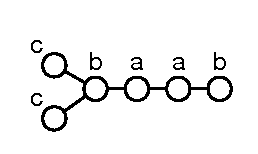
\includegraphics[height=1cm]{graph1}}) with 
vertex labeling  $\pmb{\ell}_{v_1}=\pmb{\ell}_{v_2}=c$,
$\pmb{\ell}_{v_3}=\pmb{\ell}_{v_6}=b$ and $\pmb{\ell}_{v_4}=\pmb{\ell}_{v_5}=a$, and adjacency and degree matrix 
$$
\mathbf{A}:=\begin{bmatrix}
0 & 0 & 1 & 0 & 0 & 0\\
0 & 0 & 1 & 0 & 0 & 0\\
1 & 1 & 0 & 1 & 0 & 0\\
0 & 0 & 1 & 0 & 1 & 0\\
0 & 0 & 0 & 1 & 0 & 1\\
0 & 0 & 0 & 0 & 1 & 0
\end{bmatrix}\text{ and } 
\mathbf{D}:=
\begin{bmatrix}
1 & 0 & 0 & 0 & 0 & 0\\
0 & 1 & 0 & 0 & 0 & 0\\
0 & 0 & 3 & 0 & 0 & 0\\
0 & 0 & 0 & 2 & 0 & 0\\
0 & 0 & 0 & 0 & 2 & 0\\
0 & 0 & 0 & 0 & 0 & 1
\end{bmatrix},
$$
respectively. 
We consider $\mathbf{F}^{(1)}:=\sigma(\tilde{\mathbf{D}}^{-1/2}(\mathbf{A}+\mathbf{I})\tilde{\mathbf{D}}^{-1/2}\mathbf{F}^{(0)}\mathbf{W}^{(0)})$ with  $
\mathbf{F}^{(0)}=
\left[\begin{smallmatrix}
1 & 0 & 0\\
1 & 0 & 0\\
0 & 1 & 0\\
0 & 0 & 1\\
0 & 0 & 1\\
0 & 1 & 0\\
\end{smallmatrix}\right]
$ and choose $\mathbf{W}^{(0)}=\left[\begin{smallmatrix}
1 & 0 & 0\\
0 & 1 & 0\\
0 & 0 & 1
\end{smallmatrix}\right]$. 
We remark that $\pmb{\ell}^{(0)}:=\pmb{\ell}\equiv \mathbf{F}^{(0)}$.
It can be verified that
$$
\mathbf{F}^{(1)}=\sigma\left(\begin{bmatrix}
\frac{1}{2} & \frac{1}{2\sqrt{2}}& 0\\
\frac{1}{2} & \frac{1}{2\sqrt{2}}& 0\\
\frac{1}{2\sqrt{2}} & \frac{1}{4}& \frac{1}{
2\sqrt{3}}\\
0 & \frac{1}{2\sqrt{3}}& \frac{2}{
3}\\
0 & \frac{1}{\sqrt{6}}& \frac{2}{
3}\\
0 & \frac{1}{2}& \frac{1}{
\sqrt{6}}
\end{bmatrix}\right).
$$
Suppose that $\sigma$ is the ReLU activation function. Then, we observe that
$\mathbf{F}^{(1)}_{v_4\bullet}\neq \mathbf{F}^{(1)}_{v_5\bullet}$. 
We note, however, that $\pmb{\ell}^{(1)}_{v_4}=(a,\{a,b\})=\pmb{\ell}^{(1)}_{v_5}$.
Hence, $\pmb{\ell}^{(1)}\not\sqsubseteq \mathbf{F}^{(1)}$ and this architecture is not bounded by WL.
\openprob{Is there a simple example for the one below?}
\qed
% It can, however, be verified that $\pmb{\ell}^{(2)}\sqsubseteq \mathbf{F}^{(1)}$.
% \todo{The latter inclusion needs to be verified}\qed
\end{example}
We will next provide an upper bound for  GNN architectures of the form~(\ref{eq:architecture}) by revising the labeling used in the graph.


\subsection{A general bound}\label{subsec:generalupb}
As we have seen above, for a fair comparison with GNNs of the form~(\ref{eq:architecture}), the WL process needs to have access to the information in the $\mathbf{L}$ and $\mathbf{R}$ matrices. To this aim we extend the set $\Sigma$ of labels.
Let  $(G,\pmb{\ell})$ be a labeled graph and assume that $\pmb{\ell}:V\to \Sigma$. Given $\mathbf{L}$, $\mathbf{R}$  we define $L:=\{ \mathbf{L}_{vv} \mid v\in V\}$ and
$R:=\{ \mathbf{R}_{vv} \mid v\in V\}$.
We define the set $\hat \Sigma$ of \textit{extended labels} as $\hat \Sigma:=\Sigma \cup \Sigma\times L\times R$. Given $(G,\pmb{\ell})$, we consider labeled graph $(G,\hat{\pmb{\ell}})$ with labeling
$$
\hat{\pmb{\ell}}_v:=\langle \pmb{\ell}_v, \mathbf{L}_{vv},\mathbf{R}_{vv}\rangle,
$$
for $v\in V$.
We can now bound the expressive power of  GNN architecture of the form~(\ref{eq:architecture}) by WL \textit{provided that we use the extended labels}. As before, we denote by 
$\hat{\pmb{\ell}}{}^{(t)}$ the labeling obtain after $t$ steps of the WL algorithm on $(G,\hat{\pmb{\ell}})$, starting from $\hat{\pmb{\ell}}{}^{(0)}:=\hat{\pmb{\ell}}$.

\begin{theorem}\label{thm:generalbound}
Let $(G,\pmb{\ell})$ be a labeled graph and assume that $\pmb{\ell}\sqsubseteq\mathbf{F}^{(0)}$.
Then, GNN architectures of the form~(\ref{eq:architecture}) are bounded by WL on $(G,\hat{\pmb{\ell}})$.
\end{theorem}
\begin{proof}
We show the upper bound by WL by induction on the number of iterations. For $t=0$, we have, by assumption, that 
$\pmb{\ell}\sqsubseteq \mathbf{F}^{(0)}$. Clearly,
$\hat{\pmb{\ell}}{}^{(0)}\sqsubseteq \pmb{\ell}$ and hence also 
$\hat{\pmb{\ell}}{}^{(0)}\sqsubseteq\mathbf{F}^{(0)}$. We next assume that the induction hypothesis holds for $t\geq 0$ and consider $t+1$. We need to show that 
$\hat{\pmb{\ell}}{}^{(t+1)}_v=\hat{\pmb{\ell}}{}^{(t+1)}_w$ implies that $\mathbf{F}^{(t+1)}_{v\bullet}=\mathbf{F}^{(t+1)}_{w\bullet}$. By definition,
$\hat{\pmb{\ell}}{}^{(t+1)}_v=\hat{\pmb{\ell}}{}^{(t+1)}_w$ implies
$\hat{\pmb{\ell}}{}^{(t)}_v=\hat{\pmb{\ell}}{}^{(t)}_w$ and 
$$
\ldbl \hat{\pmb{\ell}}{}^{(t)}_u \st u \in N_G(v) \rdbl=
 \ldbl \hat{\pmb{\ell}}{}^{(t)}_u \st u \in N_G(w) \rdbl.$$
 Since $\hat{\pmb{\ell}}{}^{(t)}\sqsubseteq \hat{\pmb{\ell}}{}^{(t-1)}\sqsubseteq \cdots\sqsubseteq \hat{\pmb{\ell}}{}^{(0)}$, this implies that
 $\hat{\pmb{\ell}}{}^{(0)}_v=\hat{\pmb{\ell}}{}^{(0)}_w$ and that there is a bijection $b:N_G(v)\to N_G(w):u\mapsto u'$ such that $\hat{\pmb{\ell}}{}^{(t)}_u=\hat{\pmb{\ell}}{}^{(t)}_{u'}$ and hence also 
 $\hat{\pmb{\ell}}{}^{(0)}_u=\hat{\pmb{\ell}}{}^{(0)}_{u'}$. From the definition of $\hat{\pmb{\ell}}{}^{(0)}$, $\hat{\pmb{\ell}}{}^{(0)}_v=\hat{\pmb{\ell}}{}^{(0)}_w$ implies that
 $\mathbf{L}_{vv}=\mathbf{L}_{ww}$ and
 $\mathbf{R}_{vv}=\mathbf{R}_{ww}$. Similarly, for every $u\in N_G(v)$ and corresponding $u'\in N_G(w)$,
$\hat{\pmb{\ell}}{}^{(0)}_u=\hat{\pmb{\ell}}{}^{(0)}_{u'}$ implies that   $\mathbf{L}_{uu}=\mathbf{L}_{u'u'}$ and $\mathbf{R}_{uu}=\mathbf{R}_{u'u'}$. By the induction hypothesis we also have that
 $\mathbf{F}^{(t)}_{v\bullet}=\mathbf{F}^{(t)}_{w\bullet}$, and for every $u\in N_G(v)$
   and corresponding $u'\in N_G(w)$, $\mathbf{F}^{(t)}_{u\bullet}=\mathbf{F}^{(t)}_{u'\bullet}$. It now suffices to observe that
  \begin{align*}
	  \mathbf{F}^{(t+1)}_{v\bullet}&=\sigma\Biggl(\mathbf{F}^{(t-1)}_{v\bullet}\mathbf{W}_1^{(t-1)}+\mathbf{L}_{vv}\biggl(\Bigl(\sum_{u\in N_G(v)} \mathbf{R}_{uu}\mathbf{F}^{(t)}_{u\bullet}\Bigr)+p\mathbf{R}_{vv}\mathbf{F}^{(t)}_{v\bullet}\biggr)\mathbf{W}^{(t)}+ q\mathbf{J}_{v\bullet}\Biggr)\\
	 & =\sigma\Biggl(\mathbf{F}^{(t-1)}_{w\bullet}\mathbf{W}_1^{(t-1)}+\mathbf{L}_{ww}\biggl(\Bigl(\!\!\sum_{u'\in N_G(w)}\!\! \mathbf{R}_{u'u'}\mathbf{F}^{(t)}_{u'\bullet}\Bigr)+p\mathbf{R}_{ww}\mathbf{F}^{(t)}_{w\bullet}\biggr)\mathbf{W}^{(t)}+ q\mathbf{J}_{w\bullet}\Biggr)\\
	  &=\mathbf{F}^{(t+1)}_{w\bullet},
\end{align*}
as desired.
\end{proof}

\begin{example}\label{ex3}\normalfont
	Continuing with Example~\ref{ex1}, $\hat{\pmb{\ell}}_v:=\langle a,1,1\rangle$ and $\hat{\pmb{\ell}}_w:=\langle a,1,2\rangle$. Hence, $\hat{\pmb{\ell}}{}^{(1)}_v:=(\langle a,1,1\rangle,\{\langle a,1,2\rangle\})$ and $\hat{\pmb{\ell}}{}^{(1)}_w:=(\langle a,1,2\rangle,\{\langle a,1,1\rangle\})$ and $v$ and $w$ are labeled differently in the first step of WL, starting from $\hat{\pmb{\ell}}{}^{(0)}:=\hat{\pmb{\ell}}$. Clearly,
	$\hat{\pmb{\ell}}{}^{(1)}\sqsubseteq \mathbf{F}^{(1)}$ with $\mathbf{F}^{(1)}=\left[\begin{smallmatrix}\sigma(2)\\\sigma(1)\end{smallmatrix}\right]$.
	Continuing with Example~\ref{ex2}, 
$\hat{\pmb{\ell}}_{v_1}=\hat{\pmb{\ell}}_{v_1}:=\langle c, \frac{1}{\sqrt{2}},\frac{1}{\sqrt{2}}\rangle$,
 $\hat{\pmb{\ell}}_{v_3}=\langle b, \frac{1}{\sqrt{4}},\frac{1}{\sqrt{4}}\rangle$, $\hat{\pmb{\ell}}_{v_4}=\hat{\pmb{\ell}}_{v_5}=\langle a, \frac{1}{\sqrt{3}},\frac{1}{\sqrt{3}}\rangle$, and $\hat{\pmb{\ell}}_{v_6}=\langle b,\frac{1}{\sqrt{2}},\frac{1}{\sqrt{2}}\rangle$. Hence, whereas $\pmb{\ell}^{(1)}_{v_4}=\pmb{\ell}^{(1)}_{v_5}$ we now have that
$$
\hat{\pmb{\ell}}{}^{(1)}_{v_4}:=(\langle a, \frac{1}{\sqrt{3}},\frac{1}{\sqrt{3}}\rangle,\{
\langle a, \frac{1}{\sqrt{3}},\frac{1}{\sqrt{3}}\rangle,\langle b, \frac{1}{\sqrt{4}},\frac{1}{\sqrt{4}}\rangle\})
\neq
\hat{\pmb{\ell}}{}^{(1)}_{v_5}:=(\langle a, \frac{1}{\sqrt{3}},\frac{1}{\sqrt{3}}\rangle,\{
\langle a, \frac{1}{\sqrt{3}},\frac{1}{\sqrt{3}}\rangle,\langle b, \frac{1}{\sqrt{2}},\frac{1}{\sqrt{2}}\rangle\}).
$$	It can be verified that $\hat{\pmb{\ell}}{}^{(1)}\sqsubseteq \mathbf{F}^{(1)}$.
	\qed
\end{example}

We will complement Theorem~\ref{thm:generalbound}  with the corresponding lower bound in Section~\ref{sec:lowerb}. In fact, we verify the lower bound already for a slightly simpler class of GNNs than those of the form~(\ref{eq:architecture}).
\floris{It seems that we need lower bounds for two classes (see next section.) So this may need to be revised.}
\begin{theorem}\label{thm:lowerb_general}
The class of GNNs of the form 
\begin{equation}
\mathbf{F}^{(t)}:=\sigma\left(\mathbf{L}(\mathbf{A}+p\mathbf{I})\mathbf{R}\mathbf{F}^{(t-1)}\mathbf{W}^{(t-1)} + q\mathbf{J}\right), \label{eq:architecture_lb}
\end{equation}
is WL-strong, where WL now starts from $(G,\hat{\pmb{\ell}})$. Here, $\sigma$ can be either the sign or the ReLU activation function.
\end{theorem}
This class of GNNs differs from GNNs of the form~(\ref{eq:architecture}) by eliminating  the weight matrices $\mathbf{W}_1^{(t)}$.


\subsection{Special cases}\label{subsec:specialcases}
We next observe that in some cases one can still bound  GNNs of the form~(\ref{eq:architecture}) in terms of WL using the given labeling $\pmb{\ell}$ instead of
$\hat{\pmb{\ell}}$ on $G$. 

% A trivial case for which this holds are adjacency GNNs:
% \begin{description}
%  \item[\textit{Adjacency} (A-GNN):]
% % $\mathbf{L}=\mathbf{R}:=\mathbf{I}$, $p=q:=0$. Hence,
% $
% \mathbf{F}^{(t)}:=\sigma\left(\mathbf{A}\mathbf{F}^{(t-1)}\mathbf{W}^{(t)}\right).
% $
% \end{description}
%
% Indeed, if we consider the adjacency architecture then
% $\hat{\pmb{\ell}}_v:=\langle \pmb{\ell}_v,1,1\rangle$ and thus $\hat{\pmb{\ell}}\equiv\pmb{\ell}$. In this case, the architecture will be bounded by 1-WL
% in the usual way, i.e., starting from $\pmb{\ell}^{(0)}:=\pmb{\ell}$. This holds more generally.
For example, consider GNNs of the form~\ref{eq:groheGNNwithJ}. Here, we have that $\mathbf{L}=\mathbf{R}=\mathbf{I}$. As consequence, for any labeled graph $(G,\pmb{\ell})$
we have that  $\hat{\pmb{\ell}}_v:=\langle \pmb{\ell}_v,1,1\rangle$ and thus $\hat{\pmb{\ell}}\equiv\pmb{\ell}$. In this case, the GNN will be bounded by 1-WL in the usual way, i.e., starting from $\pmb{\ell}^{(0)}:=\pmb{\ell}$. 

\begin{corollary}\label{cor:adjacency}
GNNs of the form~(\ref{eq:architecture}) for which 
$\pmb{\ell}\sqsubseteq\hat{\pmb{\ell}}$ holds, for any labeled graph $(G,\pmb{\ell})$, are bounded by WL, starting from $\pmb{\ell}^{(0)}:=\pmb{\ell}$. 
% In particular, the adjacency architecture is bounded by 1-WL.
\end{corollary}
\begin{proof}
For any labeled graph $(G,\pmb{\ell})$ we always have that $\hat{\pmb{\ell}}\sqsubseteq \pmb{\ell}$. Hence, the assumption $\pmb{\ell}\sqsubseteq\hat{\pmb{\ell}}$ implies that $\pmb{\ell}\equiv\hat{\pmb{\ell}}$. As a consequence, $\pmb{\ell}^{(t)}\equiv \hat{\pmb{\ell}}{}^{(t)}$ for all $t\geq 0$. Theorem~\ref{thm:generalbound} then implies $\hat{\pmb{\ell}}{}^{(t)}\sqsubseteq \mathbf{F}^{(t)}$, and hence also $\pmb{\ell}^{(t)}\sqsubseteq\mathbf{F}^{(t)}$.
\end{proof}
Intuitively, if $\pmb{\ell}\sqsubseteq\hat{\pmb{\ell}}$ holds for any labeled graph $(G,\pmb{\ell})$, then this implies that the matrices $\mathbf{L}$ and $\mathbf{R}$ must
be constant. Indeed, just consider the uniform labeling $\pmb{\ell}_v:=a$ for all $v\in V$. Then,
$\pmb{\ell}\equiv\hat{\pmb{\ell}}$ if and only if $\mathbf{L}_{vv}=\mathbf{L}_{ww}$
and $\mathbf{R}_{vv}=\mathbf{R}_{ww}$ for all vertices.
This is clearly the case for GNNs of the form~(\ref{eq:groheGNNwithJ}).
Another way of verifying Corollary~\ref{cor:adjacency} is that when $\mathbf{L}$ and $\mathbf{R}$ are constant, then GNNs of the form
~(\ref{eq:architecture}) can be seen as GNN of the form~\ref{lab:generalGNN}, and Proposition~\ref{prop:upperboundgeneral} applies.

In view of Corollary~\ref{cor:adjacency}, we remark that Theorem~\ref{thm:lowerb_general} implies that when $\mathbf{L}$ and $\mathbf{R}$ are constant matrices, the corresponding class of GNNs is WL-strong, starting from $(G,\pmb{\ell})$. This holds in particular
for the class of GNNs of the form~\ref{eq:groheGNNwithJ}. Hence, we recover the result from~\cite{grohewl} stating that GNNs of the form~\ref{eq:groheGNNwithJ} are WL-strong. Furthermore, as anticipated, the lower bound also holds for the ReLU function. We defer the details of the lower bounds to Section~\ref{sec:lowerb}.

As a second example, consider a NA-GNN+. For those GNNs, we have that $\mathbf{L}_{vv}=\frac{1}{\sqrt{1+d_v}}$
and $\mathbf{R}_{vv}=\frac{1}{\sqrt{1+d_v}}$. This implies that
for any labeled graph $(G,\pmb{\ell})$ we have that $\pmb{\ell}^{(1)}\sqsubseteq\hat{\pmb{\ell}}$
holds. Indeed, if $\pmb{\ell}^{(1)}_v=\pmb{\ell}^{(1)}_w$ then $\pmb{\ell}_v=\pmb{\ell}_w$ and for every $u\in N_G(v)$ and corresponding $u'\in N_G(w)$,
$\pmb{\ell}_u=\pmb{\ell}_{u'}$. In particular, $d_{v}=d_w$ and thus  $\pmb{\ell}^{(1)}\sqsubseteq\hat{\pmb{\ell}}$. More generally, if $\pmb{\ell}^{(1)}\sqsubseteq\hat{\pmb{\ell}}$ holds for any labeled graph $(G,\pmb{\ell})$,
then the entries of $\mathbf{L}$ and $\mathbf{R}$ must be functionally determined by the
degrees of the vertices. To see this, it suffices to consider again the uniform labeling
$\pmb{\ell}_v:=a$ for all $v\in V$. Then, $\pmb{\ell}^{(1)}\sqsubseteq\hat{\pmb{\ell}}$ implies that
for any two vertices $v$ and $w$, 
$$(a,\underbrace{\ldbl a, a,\ldots, a\rdbl}_{|N_G(v)|=d_v})=
(a,\underbrace{\ldbl a, a,\ldots, a\rdbl}_{|N_G(w)|=d_w}),$$
or in other words, $d_v=d_w$. So, when  $d_v=d_w$ we have $\hat{\pmb{\ell}}_v=\hat{\pmb{\ell}}_w$, or $d_v=d_w$ implies $\mathbf{L}_{vv}=\mathbf{L}_{ww}$ and $\mathbf{R}_{vv}=\mathbf{R}_{ww}$.

\begin{corollary}\label{cor:augmented2}
GNNs of the form~(\ref{eq:architecture}) for which 
$\pmb{\ell}^{(1)}\sqsubseteq\hat{\pmb{\ell}}$ holds, for any labeled graph $(G,\pmb{\ell})$, are bounded by WL, starting from $\pmb{\ell}^{(1)}$. 
\end{corollary}
\begin{proof}
If 	$\pmb{\ell}^{(1)}\sqsubseteq\hat{\pmb{\ell}}$ holds, then also 
$\pmb{\ell}^{(t+1)}\sqsubseteq\hat{\pmb{\ell}}{}^{(t)}$ holds for any $t\geq 0$. Hence,
$\pmb{\ell}^{(t+1)}\sqsubseteq \mathbf{F}^{(t)}$ 
% or $\pmb{\ell}^{(1)}\sqsubseteq\mathbf{F}^{(t-1)}$ by
by Theorem~\ref{thm:generalbound}.
\end{proof}

This upper bound holds for all special GNNs listed at the end of the previous section. Indeed,
Indeed, $\hat{\pmb{\ell}}_v:=\langle \pmb{\ell}_v,1,1\rangle$ for GNNs of the form ~(\ref{eq:groheGNNwithJ}),
$\hat{\pmb{\ell}}_v:=\langle \pmb{\ell}_v,1/d_{v},1\rangle$ for RW-GNNS,
$\hat{\pmb{\ell}}_v:=\langle \pmb{\ell}_v,1/\sqrt{d_{v}},1/\sqrt{d_{v}}\rangle$ for NA-GNNs,1-GCN's and 1-GCNs's, 
$\hat{\pmb{\ell}}_v:=\langle \pmb{\ell}_v,1/\sqrt{1+d_{v}},1\rangle$ for RW-GNN+
$\hat{\pmb{\ell}}_v:=\langle \pmb{\ell}_v,1/\sqrt{1+d_{v}},1/\sqrt{1+d_{v}}\rangle$ for NA-GNN+, as we have seen already above, and 
$\hat{\pmb{\ell}}_v:=\langle \pmb{\ell}_v,1/\sqrt{r+(1-r)d_{v}},1/\sqrt{r+(1-r)d_{v}}\rangle$ 
for NA-GNN++.

We note than when a GNN is bounded by WL, starting from $\pmb{\ell}^{(k)}$, it is also bounded by WL, starting from $\pmb{\ell}^{(k')}$ for all $k'\geq k$. The converse is not necessarily true, as is illustrated by the following example for NA-GNN+'s.
\begin{example}\label{ex4}\normalfont
Going back to  Example~\ref{ex2}, we know from Corollary~\ref{cor:augmented2} that NA-GNN+'s are bounded WL, starting from $\pmb{\ell}^{(1)}$. It can indeed be verified that in Example~\ref{ex2}, $\pmb{\ell}^{(2)}\sqsubseteq \mathbf{F}^{(1)}$. We have seen, however, that $\pmb{\ell}^{(1)}\not\sqsubseteq \mathbf{F}^{(1)}$. Hence, NA-GNN+'s are not necessarily bounded by WL, starting from $\pmb{\ell}^{(0)}$.\qed
\end{example}
It can also be verified that the previous example works for 1-GCNs's (and thus also for 1-GCN's) and NA-GNN's (and thus also NA-GNN++'s).
\begin{example}\normalfont
	Using the same setting as in Example~\ref{ex2}, it can be verified that 
	$$\mathbf{F}^{(1)}=\sigma\left(\begin{bmatrix}
	1 & 1/6 & 0\\
	1 & 1/6 & 0\\
	1/3 & 1 & 1/6\\
	0 & 1/6 & 5/4\\
	0 & 1/2 & 5/4\\
    0 & 1 & 1/2	\end{bmatrix}\right) \text{ and }
 \mathbf{F}^{(1)}=\sigma\left(\begin{bmatrix}
	0 & 1/6 & 0\\
	0 & 1/6 & 0\\
	1/3 & 0 & 1/6\\
	0 & 1/6 & 1/4\\
	0 & 1/2 & 1/4\\
    0 & 0 & 1/2	\end{bmatrix}\right), $$
	for 1-GCNs and for NA-GNNs, respectively. In both case, we see that $\pmb{\ell}^{(1)}\not\sqsubseteq \mathbf{F}^{(1)}$. Hence, these architectures are not necessarily bounded by WL, starting from $\pmb{\ell}$.\qed
\end{example}


We will complement Corollary~\ref{cor:augmented2} by the following lower bound in Section~\ref{sec:lowerb}.
\floris{Again, we need two such results, in order to capture all our GNN architectures. See next section.}

\begin{theorem}
GNNs of the form~(\ref{eq:architecture}) for which 
$\pmb{\ell}^{(1)}\sqsubseteq\hat{\pmb{\ell}}$ holds, for any labeled graph $(G,\pmb{\ell})$, are WL-strong, starting from $\pmb{\ell}^{(1)}$. 
\end{theorem}
In particular, we show this lower bound holds already for GNNs of the form~(\ref{eq:architecture_lb})
for which $\pmb{\ell}^{(1)}\sqsubseteq\hat{\pmb{\ell}}$ holds, for any labeled graph $(G,\pmb{\ell})$.



% Corollary~\ref{cor:augmented} applies for $k=1$ for the random walk, normalized adjacency, augmented random walk and augmented adjacency architectures. Indeed, for these architectures,
% $\hat{\pmb{\ell}}_v:=\langle \pmb{\ell}_v,1/d_{v},1\rangle$,
% $\hat{\pmb{\ell}}_v:=\langle \pmb{\ell}_v,1/\sqrt{d_{v}},1/\sqrt{d_{v}}\rangle$,
% $\hat{\pmb{\ell}}_v:=\langle \pmb{\ell}_v,1/\sqrt{1+d_{v}},1\rangle$, and
% $\hat{\pmb{\ell}}_v:=\langle \pmb{\ell}_v,1/\sqrt{(1+d_{v})},1/\sqrt{(1+d_{v}})\rangle$, respectively. For none of these architecture the inclusion $\pmb{\ell}\sqsubseteq \hat{\pmb{\ell}}$ necessarily holds. We note, however, that when $\pmb{\ell}^{(1)}_v=\pmb{\ell}^{(1)}_w$ then $\pmb{\ell}_v=\pmb{\ell}_w$ and for every $u\in N_G(v)$ and corresponding $u'\in N_G(w)$,
% $\pmb{\ell}_u=\pmb{\ell}_{u'}$. In particular, $d_{v}=d_w$. Hence, $\pmb{\ell}^{(1)}\sqsubseteq\hat{\pmb{\ell}}$. As a consequence,  Corollary~\ref{cor:augmented} implies:
% \begin{corollary}\label{cor:augmented2}
% The random walk, normalized adjacency, augmented random walk and augmented adjacency architectures are  bounded by 1-WL, starting from $\pmb{\ell}^{1}$.
% \end{corollary}


A careful look at the  proof of Theorem~\ref{thm:generalbound} reveals that
the roles of $\mathbf{L}$ and $\mathbf{R}$ in the GNN architectures~(\ref{eq:architecture})
are different. Indeed, if we wish to compute the feature vector $\mathbf{F}^{(t+1)}_{v\bullet}$ of a vertex $v$, then only $\mathbf{L}_{vv}$
is required from $\mathbf{L}$. By contrast, we need  $\mathbf{R}_{vv}$ and $\mathbf{R}_{uu}$ for every $u\in N_G(v)$ from $\mathbf{R}$. As it turns out,
even when $\hat{\pmb{\ell}}\not\equiv \pmb{\ell}$, it is sometimes the case that the architecture is still bounded by WL, starting from $\pmb{\ell}$. 

For example, if we take any of the GNNs for which $\mathbf{L}$ is functionally determined by
the degrees of vertices and for which $\mathbf{R}=\mathbf{I}$, then for any labeled graph $(G,\pmb{\ell})$ we have that $\pmb{\ell}^{(1)}\sqsubseteq \hat{\pmb{\ell}}$ holds, as before. In addition, however, we have that $\pmb{\ell}_v=\pmb{\ell}_w\Rightarrow \mathbf{R}_{vv}=\mathbf{R}_{ww}$. It is easy to see that this condition  corresponds to 
$\mathbf{L}$ being functionally determined by degree information, and $\mathbf{R}$ being a constant matrix. We remark that these conditions are satisfied for RW-GNNs and RW-GNN+'s
and GNNs of the form~\ref{eq:groheGNNwithJ}. 

\begin{corollary}\label{cor:weak}
	GNNs of the form~(\ref{eq:architecture}) for which 
	$\pmb{\ell}^{(1)}\sqsubseteq\hat{\pmb{\ell}}$  and
	$\pmb{\ell}^{(0)}_v=\pmb{\ell}^{(0)}_w\Rightarrow \mathbf{R}_{vv}=\mathbf{R}_{ww}$ hold,
 for any labeled graph $(G,\pmb{\ell})$, are bounded by WL, starting from $\pmb{\ell}$.
% For any $k'<k$ such that $\pmb{\ell}^{(k)}\sqsubseteq \hat{\pmb{\ell}}$ and
% $\pmb{\ell}^{(k')}_v=\pmb{\ell}^{(k')}_w\Rightarrow \mathbf{R}_{vv}=\mathbf{R}_{ww}$ hold, we have that GNN architectures of the form~(\ref{eq:architecture})  are bounded by 1-WL, starting from $\pmb{\ell}^{(k-1)}$.
\end{corollary}
\begin{proof}
We need to show that $\pmb{\ell}^{(t)}_v=\pmb{\ell}^{(t)}_w$ implies $\mathbf{F}^{(t)}_{v\bullet}=\mathbf{F}^{(t)}_{w\bullet}$ for $t\geq 0$.
We show this by induction on $t$. For $t=0$, we have by assumption that $\pmb{\ell}^{(0)}\sqsubseteq \mathbf{F}^{(0)}$.
 % and since $\pmb{\ell}^{(k-1)}\sqsubseteq\pmb{\ell}^{(0)}$ also $\pmb{\ell}^{(k-1)}\sqsubseteq\mathbf{F}^{(0)}$.
 Consider $t\geq 1$ and assume that $\pmb{\ell}^{(t)}_v=\pmb{\ell}^{(t)}_w$. This implies that $\pmb{\ell}^{(t-1)}_v=\pmb{\ell}^{(t-1)}_w$ and for every $u\in N_G(v)$ and corresponding $u'\in N_G(w)$, $\pmb{\ell}^{(t-1)}_u=\pmb{\ell}^{(t-1)}_{u'}$.
By induction, $\mathbf{F}^{(t-1)}_{v\bullet}=\mathbf{F}^{(t-1)}_{w\bullet}$ and for every $u\in N_G(v)$ and corresponding $u'\in N_G(w)$,  $\mathbf{F}^{(t-1)}_{u\bullet}=\mathbf{F}^{(t-1)}_{u'\bullet}$. 
We observe that $\pmb{\ell}^{(t)}_v=\pmb{\ell}^{(t)}_w$ implies that
$\pmb{\ell}^{(1)}_v=\pmb{\ell}^{(1)}_w$ since $t\geq 1$.
Hence,
% $\pmb{\ell}^{(1)}\sqsubseteq \hat{\pmb{\ell}}$ for $t\geq k$. Hence,
$\mathbf{L}_{vv}=\mathbf{L}_{ww}$ and $\mathbf{R}_{vv}=\mathbf{R}_{ww}$. Furthermore, 
$\pmb{\ell}^{(t-1)}_u=\pmb{\ell}^{(t-1)}_{u'}$ does not necessary implies that 
$\pmb{\ell}^{(1)}_v=\pmb{\ell}^{(1)}_w$ (e.g., when $t=1$). It does, however imply that
$\pmb{\ell}_u=\pmb{\ell}_{u'}$ and hence, by assumption, $\mathbf{R}_{uu}=\mathbf{R}_{u'u'}$. 
Hence, also $\pmb{\ell}^{(t-1)}_u=\pmb{\ell}^{(t-1)}_{u'}\Rightarrow \mathbf{R}_{uu}=\mathbf{R}_{u'u'}$.
Hence,
$\pmb{\ell}^{(t-1)}_u=\pmb{\ell}^{(t-1)}_{u'}$ implies $\mathbf{R}_{uu}=\mathbf{R}_{u'u'}$ for every $u\in N_G(v)$ and corresponding $u'\in N_G(w)$.
This suffices to conclude that 
  \begin{align*}
	  \mathbf{F}^{(t)}_{v\bullet}&=\sigma\Biggl(\mathbf{F}^{(t-1)}_{u\bullet}\mathbf{W}_1^{(t-1)}+\mathbf{L}_{vv}\biggl(\Bigl(\sum_{u\in N_G(v)} \mathbf{R}_{uu}\mathbf{F}^{(t-1)}_{u\bullet}\Bigr)+p\mathbf{R}_{vv}\mathbf{F}^{(t-k)}_{v\bullet}\biggr)\mathbf{W}^{(t-1)}+ q\mathbf{J}_{v\bullet}\Biggr)\\
	 & =\sigma\Biggl(\mathbf{F}^{(t-1)}_{v\bullet}\mathbf{W}_1^{(t-1)}+\mathbf{L}_{ww}\biggl(\Bigl(\!\!\sum_{u'\in N_G(w)}\!\! \mathbf{R}_{u'u'}\mathbf{F}^{(t-1)}_{u'\bullet}\Bigr)+p\mathbf{R}_{ww}\mathbf{F}^{(t-1)}_{w\bullet}\biggr)\mathbf{W}^{(t-1)}+ q\mathbf{J}_{w\bullet}\Biggr)\\
	  &=\mathbf{F}^{(t)}_{w\bullet},
\end{align*}
as desired.
\end{proof}

We will  show in the next section that GNNs of the form~(\ref{eq:architecture}) for which 
$\pmb{\ell}^{(1)}\sqsubseteq\hat{\pmb{\ell}}$  and 
	$\pmb{\ell}^{(0)}_v=\pmb{\ell}^{(0)}_w\Rightarrow \mathbf{R}_{vv}=\mathbf{R}_{ww}$ hold,
 for any labeled graph $(G,\pmb{\ell})$, are also WL-strong,  starting from $\pmb{\ell}$.
 
 

%
%
%
% %
% % As we will see shortly, this holds for the random walk and augmented random walk architectures.
% % % We start by identifying conditions on
% % $\hat{\pmb{\ell}}$ that result in the architecture to be only $k-1$ steps ahead of $1$-WL, rather than $k$-steps ahead as reported in Corollary~\ref{cor:augmented}.
%
% \begin{corollary}\label{cor:weak}
% For any $k'<k$ such that $\pmb{\ell}^{(k)}\sqsubseteq \hat{\pmb{\ell}}$ and
% $\pmb{\ell}^{(k')}_v=\pmb{\ell}^{(k')}_w\Rightarrow \mathbf{R}_{vv}=\mathbf{R}_{ww}$ hold, we have that GNN architectures of the form~(\ref{eq:architecture})  are bounded by 1-WL, starting from $\pmb{\ell}^{(k-1)}$.
% \end{corollary}
% We remark that the assumptions on  $\pmb{\ell}$ and $\hat{\pmb{\ell}}$ are satisfied for the
% random walk and augmented random walk architectures. Indeed, for these architectures,
% $\hat{\pmb{\ell}}_v:=\langle \pmb{\ell}_v,1/d_{v},1\rangle$ and
% $\hat{\pmb{\ell}}_v:=\langle \pmb{\ell}_v,1/\sqrt{1+d_{v}},1\rangle$, respectively. We have seen before that
% $\pmb{\ell}^{(1)}\sqsubseteq \hat{\pmb{\ell}}$. Moreover, $\pmb{\ell}^{(0)}_v=\pmb{\ell}^{(0)}_w$ implies
% $\mathbf{R}_{vv}=1=\mathbf{R}_{ww}$. Hence, Corollary~\ref{cor:weak}, for $k=1$ and $k'=0$, implies:
%
% \begin{corollary}\label{cor:augrw1wl}
% The random walk and augmented random walk architectures are bounded by 1-WL, starting from $\pmb{\ell}^{(0)}$.
% \end{corollary}
%
% It remains to show Corollary~\ref{cor:weak}. The proof is minor modification of the proof of Theorem~\ref{thm:generalbound}.


\floris{Not sure whether we want the following. It is just a generalization which basically says that if you put $k$-WL related stuff in $\mathbf{L}$ and $\mathbf{R}$ you are bounded by $\pmb{\ell}^{(k)}$. Let's discuss whether we want this. }
We conclude this section by observing that Corollaries~\ref{cor:augmented2} and~\ref{cor:weak} generalize as follows. 
\begin{corollary}\phantom{This is just a dummy line}
\begin{itemize}
\item[(a)] GNNs of the form~(\ref{eq:architecture}) for which 
	$\pmb{\ell}^{(k)}\sqsubseteq\hat{\pmb{\ell}}$  holds,
 for any labeled graph $(G,\pmb{\ell})$, are bounded by WL, starting from $\pmb{\ell}^{(k)}$.
\item[(b)] GNNs of the form~(\ref{eq:architecture}) for which 
	$\pmb{\ell}^{(k)}\sqsubseteq\hat{\pmb{\ell}}$  and
	$\pmb{\ell}^{(k')}_v=\pmb{\ell}^{(0)}_w\Rightarrow \mathbf{R}_{vv}=\mathbf{R}_{ww}$ with $k'<k$ hold,
 for any labeled graph $(G,\pmb{\ell})$, are bounded by WL, starting from $\pmb{\ell}^{(k-1)}$.
\end{itemize}	
\end{corollary}
%  $\pmb{\ell}^{(k)}\sqsubseteq\hat{\pmb{\ell}}$
% and $\pmb{\ell}^{(k)}\sqsubseteq\hat{\pmb{\ell}}$ and $$
%
% Remark: iterated degrees...
% More generally, we have the following property.
% \begin{corollary}\label{cor:augmented}
% If $\pmb{\ell}^{(k)}\sqsubseteq\hat{\pmb{\ell}}$ holds, then the GNN architecture~(\ref{eq:architecture})  is bounded by 1-WL, starting from $\pmb{\ell}^{(k)}$.
% \end{corollary}
% Intuitively, this implies that the GNN architecture is $k$-steps ahead of the 1-WL algorithm.
% More precisely, $\pmb{\ell}^{(t)}\sqsubseteq \mathbf{F}^{(t-k)}$ for $t\geq k$.
\begin{proof}
	For (a)~, if 	$\pmb{\ell}^{(k)}\sqsubseteq\hat{\pmb{\ell}}$ holds, then also 
$\pmb{\ell}^{(k+t)}\sqsubseteq\hat{\pmb{\ell}}{}^{(t)}$ holds for any $t\geq 0$. Hence,
$\pmb{\ell}^{(k+t)}\sqsubseteq \mathbf{F}^{(t)}$ or $\pmb{\ell}^{(k)}\sqsubseteq\mathbf{F}^{(t-k)}$ by Theorem~\ref{thm:generalbound}.
For (b)~, it is easily verified that the proof of Corollary~\ref{cor:weak} can be generalized to this setting.
\end{proof}
Intuitively, when $\pmb{\ell}^{(k)}\sqsubseteq\hat{\pmb{\ell}}$ holds for any labeled graph $(G,\pmb{\ell})$, then this implies that the entries in $\mathbf{L}$ and $\mathbf{R}$ are functionally determined by the so-called \textit{$k$-iterated degrees} of vertices. The $k$-iterated degree of a vertex $v$ is the label assigned by $k$-steps of  WL on the uniformily labeled graph $(G,\pmb{a})$ in which every vertex is assigned the label $a$.
Similarly, $\pmb{\ell}^{(k')}_v=\pmb{\ell}^{(0)}_w\Rightarrow \mathbf{R}_{vv}=\mathbf{R}_{ww}$ implies that the entries in $\mathbf{R}$ are functionally determined by the $k'$-iterated degrees of vertices. We illustrate this by the following example.
\begin{example}
	\floris{Show example for say, $k=2$, and $k=2$ and $k'=1$, if we think this is interesting.}
\end{example}

%!TEX root =main.tex

\section{Lower bounding the expressive power}\label{sec:lowerb}

\floris{I think we need to show a lower bound for two classes. See later.
We may need to revise this section accordingly.}

We start this section by showing Theorem~\ref{thm:lowerb_general}.
More precisely, we show that for any given labeled graph
$(G,\pmb{\ell})$, there exist parameters $p$, $q$ and weight matrices $\mathbf{W}^{(t)}$, such that when $\mathbf{F}^{(0)}\equiv \hat{\pmb{\ell}}{}^{(t)}$, then for all $t\geq 0$, $\hat{\pmb{\ell}}{}^{(t)}\equiv \mathbf{F}^{(t)}$ where
$$
\mathbf{F}^{(t)}:=\sigma\left(\mathbf{L}(\mathbf{A}+p\mathbf{I})\mathbf{R}\mathbf{F}^{(t-1)}\mathbf{W}^{(t-1)} + q\mathbf{J}\right).$$ 

To show this, we follow the same strategy as in~\cite{grohewl}.
Crucial in establishing the lower bound are the following definitions (see also~\cite{grohewl}):
\begin{definition}[row independent modulo equality]\label{def:label2}\normalfont
A matrix $\mathbf{F}$ is \textit{row-independent modulo equality} if the unique row vectors in $\mathbf{F}$ are linearly independent. \qed
\end{definition}

\begin{definition}[a good matrix]\label{def:label3}\normalfont
A matrix $\mathbf{F}$ is \textit{good relative to an other matrix} $\mathbf{F}'$ if $\mathbf{F}\equiv \mathbf{F}'$ and $\mathbf{F}$ is row-independent modulo equality.\qed
\end{definition}

To show the lower bound we will inductively show that when $\mathbf{F}^{(t-1)}$ is good relative to $\hat{\pmb{\ell}}{}^{(t-1)}$, then. there exists a weight matrix $\mathbf{W}^{(t-1)}$, such that 
$\mathbf{F}^{(t)}$ is also good relative to $\hat{\pmb{\ell}}{}^{(t)}$. This clearly suffices to infer the lower bound. 

The induction hypothesis will be shown in a number of steps, by gradually adding the different components in the GNN architecture. We start by showing that multiplication with $\mathbf{R}$ preserves the goodness of the feature matrix.

%
% We first show, by induction on $t$, that when $\mathbf{F}^{(t)}$ is good relative to $\hat{\pmb{\ell}}^{(t)}$, then there exists a constant $p$ and constants $q^{(t)}$ and weight matrices
% $\mathbf{W}^{(t)}$, such that
% $$
% \mathbf{F}^{(t+1)}:=\sigma\Bigl(\mathbf{L}(\mathbf{A}+p\mathbf{I})\mathbf{R}\mathbf{F}^{(t)}\mathbf{W}^{(t)}+q^{(t)}\mathbf{B}\Bigr)
% $$
% is also good relative to $\hat{\pmb{\ell}}^{(t+1)}$. In a next step, we show that we can choose $q^{(t)}$ uniformly across all layers.


\begin{lemma}\label{lem:rightgood}
	For any $t\geq 0$,
	If $\mathbf{F}^{(t)}$ is good relative to $\hat{\pmb{\ell}}{}^{(t)}$, then $\mathbf{R}\mathbf{F}^{(t)}$ is also good relative to $\hat{\pmb{\ell}}{}^{(t)}$.
\end{lemma}
\begin{proof}
By assumption, we have that $\mathbf{F}^{(t)}_{v\bullet}=\mathbf{F}^{(t)}_{w\bullet}$ implies 
$\hat{\pmb{\ell}}{}^{(t)}_{v}=\hat{\pmb{\ell}}{}^{(t)}_w$. Furthermore, since $\hat{\pmb{\ell}}{}^{(t)}\sqsubseteq\hat{\pmb{\ell}}{}^{(0)}$,
$\mathbf{F}^{(t)}_{v\bullet}=\mathbf{F}^{(t)}_{w\bullet}$ implies  $\hat{\pmb{\ell}}{}^{(0)}_{v}=\hat{\pmb{\ell}}{}^{(0)}_w$. This in turn means that 
$\mathbf{R}_{vv}=\mathbf{R}_{ww}$. Hence, $\mathbf{F}^{(t)}_{v\bullet}=\mathbf{F}^{(t)}_{w\bullet}$  implies that 
$\mathbf{R}_{vv}\mathbf{F}^{(t)}_{v\bullet}=\mathbf{R}_{ww}\mathbf{F}^{(t)}_{w\bullet}$.
For the converse, suppose that $\mathbf{R}_{vv}\mathbf{F}^{(t)}_{v\bullet}=\mathbf{R}_{ww}\mathbf{F}^{(t)}_{w\bullet}$ holds.
Then, $\mathbf{F}^{(t)}_{v\bullet}=\mathbf{F}^{(t)}_{w\bullet}$ since otherwise we would have to
distinct rows $\mathbf{F}^{(t)}_{v\bullet}$ and $\mathbf{F}^{(t)}_{w\bullet}$ which are linearly dependent. This contradicts the assumption that $\mathbf{F}^{(t)}$ is row-independent modulo equality.
Hence, $\mathbf{R}\mathbf{F}^{(t)}\equiv\mathbf{F}^{(t)}\equiv\hat{\pmb{\ell}}{}^{(t)}$. Using the same reasoning as above, $\mathbf{R}\mathbf{F}^{(t)}$ is also row-independent modulo equality. Indeed, suppose that the unique rows in $\mathbf{R}\mathbf{F}^{(t)}$ are linearly dependent. Then, this implies that also the unique rows in $\mathbf{F}^{(t)}$ are linearly dependent, a contradiction. 
\end{proof}

We next consider multiplication with $\mathbf{A}+q\mathbf{I}$. 

\begin{lemma}\label{lem:findingp}
If $\mathbf{F}^{(t-1)}$ is good relative to $\hat{\pmb{\ell}}{}^{(t-1)}$, then there exists a  weight matrix $\mathbf{U}^{(t-1)}$ such that 
$\mathbf{G}^{(t)}:=(\mathbf{A}+p\mathbf{I})\mathbf{F}^{(t-1)}\mathbf{U}^{(t-1)}$ is equivalent to 
$\hat{\pmb{\ell}}{}^{(t)}$. Furthermore, this holds for any $p$ such that $0<p<1$.
\end{lemma}
\begin{proof}
By assumption, $\mathbf{F}^{(t-1)}$ is row-independent modulo equality.
Suppose that $\mathbf{F}^{(t-1)}$ is an $n\times f$-matrix, with $n$ the number of vertices in $(G,\pmb{\ell})$.
Let 
$\widetilde{\mathbf{F}}^{(t-1)}$ be the $u\times f$-matrix consisting of the unique rows in $\mathbf{F}^{(t-1)}$. Because the rows in $\widetilde{\mathbf{F}}^{(t-1)}$ are linearly independent,
there exists a $f\times u$-matrix $\mathbf{U}^{(t-1)}$ such that $\widetilde{\mathbf{F}}^{(t-1)}\mathbf{U}^{(t-1)}=\mathbf{I}_{u\times u}$. By induction $\mathbf{F}^{(t-1)}\equiv\hat{\pmb{\ell}}{}^{(t-1)}$. Let $\Sigma^{(t-1)}$ be the set of  labels assigned by $\hat{\pmb{\ell}}{}^{(t-1)}$ to vertices $v\in V$. 
For any $v\in V$ and $c\in\Sigma^{(t-1)}$, we denote by $\mathbf{F}^{(t-1)}_{v\bullet}\sim c$ that
$\hat{\pmb{\ell}}{}^{(t)}_v=c$.
Then for each $v\in V$ and $c\in \Sigma^{(t-1)}$ we have:
\begin{align*}
(\mathbf{A}\mathbf{F}^{(t-1)}\mathbf{M}^{(t-1)})_{vc}&=|\{u\in N_G(v)\mid \mathbf{F}^{(t-1)}_{u\bullet}\sim c\}|.
\intertext{Furthermore,} 
p\mathbf{I}(\mathbf{F}^{(t-1)}\mathbf{M}^{(t-1)})_{vc}&=p\delta_{vc},
\end{align*}
with $\delta_{vc}=1$ if $\mathbf{F}^{(t-1)}_{v\bullet}\sim c$ and $\delta_{vc}=0$ otherwise.

We next show that $\mathbf{G}^{(t)}:=(\mathbf{A}+p\mathbf{I})\mathbf{F}^{(t-1)}\mathbf{M}^{(t-1)}$ is equivalent to $\hat{\pmb{\ell}}{}^{(t)}$. Indeed, suppose that 
$\hat{\pmb{\ell}}{}^{(t)}_v=\hat{\pmb{\ell}}{}^{(t)}_w$. Then,
$\hat{\pmb{\ell}}{}^{(t-1)}_v=\hat{\pmb{\ell}}{}^{(t-1)}_w$ and for every $u\in N_G(v)$ and corresponding $u'\in N_G(w)$, $\hat{\pmb{\ell}}{}^{(t-1)}_u=\hat{\pmb{\ell}}{}^{(t-1)}_{u'}$. Since $\mathbf{F}^{(t-1)}\equiv\hat{\pmb{\ell}}{}^{(t-1)}$ this implies for any $c\in \Sigma^{(t-1)}$,
 $\delta_{vc}=\delta_{wc}$ and 
$|\{u\in N_G(v)\mid \mathbf{F}^{(t-1)}_{u\bullet}\sim c\}|=
|\{u\in N_G(w)\mid \mathbf{F}^{(t-1)}_{u\bullet}\sim c\}|$. In other words,
$\mathbf{G}^{(t)}_{v\bullet}=\mathbf{G}^{(t)}_{w\bullet}$. Conversely,
suppose that $\mathbf{G}^{(t)}_{v\bullet}=\mathbf{G}^{(t)}_{w\bullet}$. Then, for every $c\in \Sigma^{(t-1)}$,
$|\{u\in N_G(v)\mid \mathbf{F}^{(t-1)}_{u\bullet}\sim c\}|+p\delta_{vc}=
|\{u\in N_G(w)\mid \mathbf{F}^{(t-1)}_{u\bullet}\sim c\}|+p\delta_{wc}$. We next distinguish between a number of cases. Suppose first that $\delta_{vc}=\delta_{wc}$. Then, we must have that $|\{u\in N_G(v)\mid \mathbf{F}^{(t-1)}_{u\bullet}\sim c\}|=
|\{u\in N_G(w)\mid \mathbf{F}^{(t-1)}_{u\bullet}\sim c\}|$. Since $\mathbf{F}^{(t-1)}\equiv\hat{\pmb{\ell}}^{(t-1)}$ this implies that $\hat{\pmb{\ell}}{}^{(t-1)}_v=\hat{\pmb{\ell}}{}^{(t-1)}_w$ and for every $u\in N_G(v)$ and corresponding $u'\in N_G(w)$, $\hat{\pmb{\ell}}{}^{(t-1)}_u=\hat{\pmb{\ell}}{}^{(t-1)}_{u'}$. In other words, 
$\hat{\pmb{\ell}}{}^{(t)}_v=\hat{\pmb{\ell}}{}^{(t)}_w$. By contrast, if $\delta_{vc}\neq \delta_{wc}$ then either $|\{u\in N_G(v)\mid \mathbf{F}^{(t-1)}_{u\bullet}\sim c\}|=
|\{u\in N_G(w)\mid \mathbf{F}^{(t-1)}_{u\bullet}\sim c\}|+p$ or
$|\{u\in N_G(v)\mid \mathbf{F}^{(t-1)}_{u\bullet}\sim c\}|+p=
|\{u\in N_G(w)\mid \mathbf{F}^{(t-1)}_{u\bullet}\sim c\}|$. This, however, is impossible for any $p$ such that $0<p<1$ because  $|\{u\in N_G(w)\mid \mathbf{F}^{(t-1)}_{u\bullet}\sim c\}|$ and $|\{u\in N_G(w)\mid \mathbf{F}^{(t-1)}_{u\bullet}\sim c\}|$ are integers.
\end{proof}


We remark that the previous lemma only guarantees that $\mathbf{H}^{(t)}$ is equivalent to $\hat{\pmb{\ell}}{}^{(t)}$. We show later how row-independence modulo equality is ensured.
Furthermore, the lemma is stated in terms of $\mathbf{F}^{(t)}$ instead of $\mathbf{R}\mathbf{F}^{(t)}$.
From Lemma~\ref{lem:rightgood} we know, however, that $\mathbf{F}^{(t)}\equiv\mathbf{R}\mathbf{F}^{(t)}$
so we can apply Lemma~\ref{lem:findingp} to $\mathbf{R}\mathbf{F}^{(t)}$ as well.

We next consider multiplication with $\mathbf{L}$. In the following, we let $\mathbf{G}^{(t)}:=(\mathbf{A}+p\mathbf{I})\mathbf{R}\mathbf{F}^{(t-1)}\mathbf{U}^{(t-1)}$.

% \todo{The lemma below is new. It allows to use a simplified bias matrix. Our previous argument required the bias matrix to be $\mathbf{L}\mathbf{J}$. We now only have $\mathbf{J}$. This lemma needs to be checked carefully ;-)}
\begin{lemma}\label{lemma:findp}
There exists a constant $m_p$, only dependent on $\mathbf{L}$ and the number of vertices $V$ in $G$, such that for all $p$ for which $m_p<p<1$, $\mathbf{L}\mathbf{G}^{(t)}$ is equivalent to $\hat{\pmb{\ell}}{}^{(t)}$.
\end{lemma}
\begin{proof}
	We know from Lemma~\ref{lem:findingp} that
 $\mathbf{G}^{(t)}\equiv\hat{\pmb{\ell}}{}^{(t)}$ for all $p$, $0<p<1$.
	Suppose that $\hat{\pmb{\ell}}{}^{(t)}_v=\hat{\pmb{\ell}}{}^{(t)}_w$, or equivalently, that	$\mathbf{G}^{(t)}_{v\bullet}=\mathbf{G}^{(t)}_{w\bullet}$. This implies that
	  $\hat{\pmb{\ell}}{}^{(0)}_v=\hat{\pmb{\ell}}{}^{(0)}_w$. In particular, we must have that $\mathbf{L}_{vv}=\mathbf{L}_{ww}$. This in turn implies
$\mathbf{L}_{vv}\mathbf{G}^{(t)}_{v\bullet}=\mathbf{L}_{ww}\mathbf{G}^{(t)}_{w\bullet}$.

We next describe a procedure of how to obtain $m_p$. Later on, we define $m_p$ directly
from $\mathbf{L}$ and $n$.

Initially, $m_p=0$. Then, we update $m_p$ as long as
$\mathbf{L}\mathbf{G}^{(t)}\not\equiv\hat{\pmb{\ell}}{}^{(t)}$. We have just seen that
$\hat{\pmb{\ell}}{}^{(t)}\sqsubseteq \mathbf{L}\mathbf{G}^{(t)}$ for all $p$, $0<p<1$.
Hence, we update $m_p$ as long as $\mathbf{L}\mathbf{G}^{(t)}\not\sqsubseteq\hat{\pmb{\ell}}{}^{(t)}$.
The latter implies that
there exists two vertices $v,w\in V$ such that
\begin{equation}
\mathbf{L}_{vv}\mathbf{G}^{(t)}_{v\bullet}=\mathbf{L}_{ww}\mathbf{G}^{(t)}_{w\bullet},\label{eq:contra}
\end{equation}
but $\hat{\pmb{\ell}}{}^{(t)}_v\neq \hat{\pmb{\ell}}{}^{(t)}_w$, or equivalently, $\mathbf{G}^{(t)}_{v\bullet}\neq \mathbf{G}^{(t)}_{w\bullet}$.
Clearly, in this case $\mathbf{L}_{vv}\neq\mathbf{L}_{ww}$. Hence, the equality~(\ref{eq:contra}) implies that for every $c\in\Sigma^{(t-1)}$, either
(i)~$\mathbf{G}^{(t)}_{vc}=0=\mathbf{G}^{(t)}_{wc}$; or (ii)~ $0\neq \mathbf{G}^{(t)}_{vc}\neq \mathbf{G}^{(t)}_{wc}\neq 0$. Here, $\Sigma^{(t-1)}$ is the set of labels as used in the proof of  Lemma~\ref{lem:findingp}. Furthermore, for all $c\in\Sigma^{(t-1)}$ for which (ii) holds, 
\begin{equation}
\frac{\mathbf{G}^{(t)}_{vc}}{\mathbf{G}^{(t)}_{wc}}=\frac{\mathbf{L}_{ww}}{\mathbf{L}_{vv}}\neq 1.\label{eq:ratio}
\end{equation}
Let $\alpha:=\frac{\mathbf{L}_{ww}}{\mathbf{L}_{vv}}$.
We also observe that, since $p$ occurs in precisely one entry in $\mathbf{G}^{(t)}_{v\bullet}$ and $\mathbf{G}^{(t)}_{w\bullet}$, there is at least one $c\in\Sigma^{(t-1)}$ for which (ii) holds. Furthermore, the proof of  Lemma~\ref{lem:findingp} tells precisely how the elements $\mathbf{G}^{(t)}_{vc}$ and $\mathbf{G}^{(t)}_{wc}$ look like. That is, these entries are of the form 
$i$ or $i+p$ for $i\in[1,n]$ with $n=|V|$. If we consider equation~(\ref{eq:ratio}) for
the entries containing $p$ we are in one of the following three cases:
$$
\text{(a) } \frac{i+p}{j}=\alpha
\text{; (b) } \frac{i}{j+p}=\alpha
\text{; or (c) } \frac{i+p}{j+p}=\alpha
$$
for some $i,j\in[1,n]$. Hence, in case (a)~$p=\alpha j- i$, in case (b)~$p=\frac{i-\alpha j}{\alpha}$, and in case (c)~$p=\frac{\alpha(j-i)}{1-\alpha}$. It now suffices to update
$m_p=\max\{m_p,\alpha j- i,\frac{i-\alpha j}{\alpha},\frac{\alpha(j-i)}{1-\alpha}\}$ and
hence for any $p>m_p$, equation~(\ref{eq:ratio}) is not satisfied anymore for $v$ and $w$.
We proceed in this way, as long is there exists a pair of vertices  $v,w\in V$ for which equation~\ref{eq:contra} holds  but $\hat{\pmb{\ell}}{}^{(t)}_v\neq \hat{\pmb{\ell}}{}^{(t)}_w$. Note that $m_p$ has been updated for a particular pair of vertices, that pair will not need to considered anymore. The final $m_p$ is the value when
for all vertices $v,w\in V$, equation~\ref{eq:contra} implies $\hat{\pmb{\ell}}{}^{(t)}_v= \hat{\pmb{\ell}}{}^{(t)}_w$. In other words, when $\mathbf{L}\mathbf{G}^{(t)}\sqsubseteq\hat{\pmb{\ell}}{}^{(t)}$ holds.

It should be clear now that we can define $m_p$ more roughly, as follows.
First, define $L':=\{\frac{\mathbf{L}_{vv}}{\mathbf{L}_{ww}}\mid \mathbf{L}_{vv}\neq\mathbf{L}_{ww}, v,w\in V\}$. Then, consider
\begin{align*}
P_1&:=\left\{ \alpha j -i \mid 0\leq \alpha i -j < 1, i,j\in[1,n],\alpha\in L'\right\}\\
P_2&:=\left\{ \frac{i -\alpha j}{\alpha} \mid 0\leq \frac{i -\alpha j}{\alpha} < 1, i,j\in[1,n],\alpha\in L'\right\}\\
P_3&:=\left\{ \frac{\alpha(j-i)}{1-\alpha} \mid 0\leq \frac{\alpha(j-i)}{1-\alpha} < 1, i,j\in[1,n],\alpha\in L'\right\}
\end{align*}
and let $m_p=\max\{P_1\cup P_2\cup P_3\cup\{0\}\}$. In other words, we just consider all possible $p$ values as determined before that could lead to 
$\mathbf{L}\mathbf{G}^{(t)}\not\sqsubseteq\hat{\pmb{\ell}}{}^{(t)}$ and eliminate these possibility by choosing $p$ large enough, as explained earlier.
%
% We will sho
% consider the set $L':=\{\frac{\mathbf{L}_{vv}}{\mathbf{L}_{ww}}\mid \mathbf{L}_{vv}\neq\mathbf{L}_{ww}, v,w\in V\}$. We remark this, by assumption $L_{vv}\neq 0$ for any $v\in V$ so we do not have zero denominators. We define $m_p$ as follows.
% Initially, we set $m_p:0$. Then,
% suppose that
% $\mathbf{L}_{vv}\mathbf{G}^{(t)}_{v\bullet}=\mathbf{L}_{ww}\mathbf{G}^{(t)}_{w\bullet}$ for some
% vertices $v,w\in V$. We will show how to change $m_p$ such for all $p$ satisfying
% $m_p<p<1$, $\mathbf{L}_{vv}\mathbf{G}^{(t)}_{v\bullet}\neq \mathbf{L}_{ww}\mathbf{G}^{(t)}_{w\bullet}$.
% (Recall from the proof of  Lemma~\ref{lem:findingp} that every $\mathbf{G}^{(t)}_{v\bullet}$
% has at least one entry containing $p$.)
%
%
%
%
% We next consider $M'=\{\frac{\mathbf{G}^{(t)}_{wc}}{\mathbf{G}^{(t)}_{vc}}\mid \mathbf{G}^{(t)}_{vc}\neq \mathbf{G}^{(t)}_{wc},\mathbf{G}^{(t)}_{vc}\neq 0, v,w\in V,c\in\Sigma^{(t-1)}\}$, where $\Sigma^{(t-1)}$ is the set of labels as used in the proof of  Lemma~\ref{lem:findingp}. From that proof we also know precisely how the ratio's in $M'$ look like. That is, every such a ratio is of the form
% $\frac{i+p}{j}$, $\frac{i}{j+p}$ or $\frac{i+p}{j+p}$ for $i,j\in[0,|V|]$.
%
%  Let
% $G$ be the collection of all these fractions and choose $p$ such that $G\cap L'=\emptyset$
% (almost any $p$ will do.). Suppose now that $\hat{\pmb{\ell}}^{(t)}_v\neq \hat{\pmb{\ell}}^{(t)}_w$
% and thus $\mathbf{G}^{(t)}_{v\bullet}\neq \mathbf{G}^{(t)}_{w\bullet}$. Suppose, for the sake of
% contradiction that $\mathbf{L}_{vv}\mathbf{G}^{(t)}_{v\bullet}=\mathbf{L}_{ww}\mathbf{G}^{(t)}_{w\bullet}$. This implies
% that the non-zero entries in $\mathbf{G}^{(t)}_{v\bullet}$ correspond to non-zero (but possibly different)
% entries in $\mathbf{G}^{(t)}_{w\bullet}$. We are guaranteed at least one non-zero entry in $\mathbf{G}^{(t)}_{v\bullet}$ which contains $p$. Assume that this entry is of the form $i+p$. Then,
% the corresponding non-zero entry in $\mathbf{G}^{(t)}_{w\bullet}$ is of the form $j$ or $j+p$. We also know that  $\mathbf{G}^{(t)}_{v\bullet}\neq \mathbf{G}^{(t)}_{w\bullet}$ and $\mathbf{L}_{vv}\mathbf{G}^{(t)}_{v\bullet}=\mathbf{L}_{ww}\mathbf{G}^{(t)}_{w\bullet}$ implies that
% $\mathbf{L}_{vv}\neq\mathbf{L}_{ww}$. Hence, the assumption implies that
% $\frac{\mathbf{L}_{vv}}{\mathbf{L}_{ww}}=\frac{j}{i+p}$ or $\frac{\mathbf{L}_{vv}}{\mathbf{L}_{ww}}=\frac{j+p}{i+p}$. In other words, $G\cap L'\neq\emptyset$, a contradiction.
\end{proof}

At this point, we know that when $\mathbf{F}^{(t-1)}$ is good relative to $\hat{\pmb{\ell}}{}^{(t-1)}$ then there exists a $\mathbf{M}^{(t-1)}$ such that $\mathbf{H}^{(t)}:=\mathbf{L}(\mathbf{A}+p\mathbf{I})\mathbf{R}\mathbf{F}^{(t-1)}\mathbf{M}^{(t-1)}$
is equivalent to $\hat{\pmb{\ell}}{}^{(t)}$, and this for any $p$ such that $m_p<p<1$.
We now come to the point that will ensure that there exists a $q$ and $\mathbf{N}^{(t-1)}$ such that
$$
\mathbf{F}^{(t)}:=\sigma(\mathbf{L}(\mathbf{A}+p\mathbf{I})\mathbf{R}\mathbf{F}^{(t-1)}\underbrace{\mathbf{M}^{(t-1)}\mathbf{N}^{(t-1)}}_{\mathbf{W}^{(t-1)}}+q\mathbf{J})$$
 is good relative to $\hat{\pmb{\ell}}{}^{(t)}$, where $\sigma$ is either the sign or the ReLU activation function. We here follow closely the approach taken in~\cite{grohewl}.
Lemma 9 in~\cite{grohewl} states:

 \begin{lemma}[Lemma 9 in~\cite{grohewl}]\label{lem:signlemma9}
  Let
  $\mathbf{B}\in \Nb^{u\times f}$ be a matrix in which all
  rows are pairwise disjoint.
%  \footnote{I believe that this can be
%  guaranteed in 1-WL}).\todo{G: with our extended features we actually guarantee this for free by adding the 1 column; also, t as dimension is a bad choice\ldots}
  Then there exists a matrix $\mathbf{N}$ 
  such that $\text{\normalfont sign}(\mathbf{BN}-\mathbf{J})$ is
  non-singular.
\end{lemma}
Although~\cite{grohewl} also consider the ReLU activation function, they simulate each application of the ReLu function by two applications of the sign function. As a consequence,
the overall number of layers doubled. A more direct approach can be applied, however. More
precisely, we show the following:
 \begin{lemma}\label{lem:relulemma9}
  Let
  $\mathbf{B}\in \Nb^{u\times f}$ be a matrix in which all
  rows are pairwise disjoint and such that no row consists entirely
  out of zeroes.
%  \footnote{I believe that this can be
%  guaranteed in 1-WL}).\todo{G: with our extended features we actually guarantee this for free by adding the 1 column; also, t as dimension is a bad choice\ldots}
  Then there exists a matrix $\mathbf{N}$ and a constant $q$
  such that $\text{\normalfont ReLU}(\mathbf{BN}-q\mathbf{J})$ is
  non-singular. In fact, if we denote by $M$ the maximal entry in $\mathbf{B}$,
  any $q$ such that  $\frac{M^f-1}{M^f} < q < 1$ will do.
\end{lemma}
\begin{proof}
Let $M$ be the maximal entry in $\mathbf{B}$ and consider the column vector $\mathbf{z}=(1,M,M^2,\ldots,M^{f-1})^{\textsc{t}}$.
Then each entry in $\mathbf{b}=\mathbf{B}\mathbf{z}$ is positive and they are all pairwise distinct. 
Let $\mathbf{P}$ be a permutation matrix in $\Rb^{u\times u}$ such that $\mathbf{b}'=\mathbf{P}\mathbf{b}$ is such that  $\mathbf{b}'=(b_1',b_2',\ldots,b_u')^{\textsc{	t}}\in\Rb^{u\times 1}$ with $ b_1'> b_2'>\cdots > b_u'>0$. 
Consider the $\mathbf{x}=\left(\frac{1}{b_1'},\ldots,\frac{1}{b_u'}\right)\in \Rb^{1\times u}$. Then, for $\mathbf{C}=\mathbf{b}'\mathbf{x}$
$$
\mathbf{C}_{ij}=\frac{b_i'}{b_j'}  \text{ and } \mathbf{C}_{ij}=\begin{cases}  1 & \text{if $i=j$}\\
>1 & \text{if $i<j$}\\
< 1 & \text{if $i>j$}.
\end{cases}
$$
Let $q$ be the greatest value  in $\mathbf{C}$ smaller than $1$.
% G: I think the m instantiated here is not correct
%, i.e., $m=\frac{b_s}{b_1}$.
Consider $\mathbf{E}=\mathbf{C}- q\mathbf{J}$.
Then,
$$
\mathbf{E}_{ij}=\frac{b_i'}{b_j'}- q \text{ and } \mathbf{E}_{ij}=\begin{cases}  1-m & \text{if $i=j$} \\
> 0 & \text{if $i<j$}\\
\leq 0  & \text{if $i>j$}.
\end{cases}
$$
As a consequence,
$$
\text{ReLU}(\mathbf{E})_{ij}=\begin{cases}  1-q & \text{if $i=j$}\\
>0 & \text{if $i<j$}\\
0  & \text{if $i>j$}.
\end{cases}
$$
This is an upper triangular matrix with (nonzero) value $1-q$ on its diagonal. It is therefore non-singular. 
We observe that $\mathbf{Q}\text{ReLU}(\mathbf{E})=\text{ReLU}(\mathbf{Q}\mathbf{E})$ for any row permutation $\mathbf{Q}$. Furthermore, non-singularity is preserved under row permutations and $\mathbf{Q}\mathbf{J}=\mathbf{J}$. Hence, if we define $\mathbf{N}=\mathbf{z}\mathbf{x}$ and use the permutation matrix $\mathbf{P}$:
\begin{align*}
\mathbf{P}\text{ReLU}(\mathbf{B}\mathbf{N}-q\mathbf{J})&=
\text{ReLU}(\mathbf{P}\mathbf{B}\mathbf{z}\mathbf{x}-q\mathbf{P}\mathbf{J})=\text{ReLU}(\mathbf{E}-q\mathbf{J}),
\end{align*}
we have that $\text{ReLU}(\mathbf{B}\mathbf{N}-q\mathbf{J})$ is non-singular, as desired.
%So, the lemma is satisfied by taking $m$ as above and
%%$m=b_s/b_1$ and % G: this still looks wrong
%$\mathbf{X}=\mathbf{z}\mathbf{x}$.
To validate second claim in the statement of the lemma, it suffices to observe that every
in $\mathbf{b'}$ is bounded by $M^f$ and hence every 
$\frac{b_i'}{b_j'}$ in $\mathbf{C}$ such that $\frac{b_i'}{b_j'}<1$ is bounded by
$\frac{M^f-1}{M^f}$. Choosing $q$ larger than this number clearly
ensures the correctness of the above construction.
\end{proof}

We are now almost at the end of the lower bound proof. Indeed,
consider the matrix $\widetilde{\mathbf{H}}{}^{(t)}$ consisting of the unique rows
of $\mathbf{H}^{(t)}:=\mathbf{L}(\mathbf{A}+p\mathbf{I})\mathbf{R}\mathbf{F}^{(t-1)}\mathbf{M}^{(t-1)}$. Suppose that $\widetilde{\mathbf{H}}{}^{(t)}$ is of dimension $u\times f$.
Then, when $\sigma$ is the sign function, Lemma~\ref{lem:signlemma9} implies 
the existence of an $f\times u$-matrix $\mathbf{N}^{(t)}$ such that
$\sigma(\widetilde{\mathbf{H}}{}^{(t)}\mathbf{N}^{(t)}-\mathbf{J})$ is non-singular
and thus is row-independent. As a consequence, 
$\mathbf{F}^{(t)}:=\sigma(\mathbf{H}{}^{(t)}\mathbf{N}^{(t)}-\mathbf{J})$ is 
row-independent modulo equality. Since  $\mathbf{H}{}^{(t)}\equiv\hat{\pmb{\ell}}{}^{(t)}$
we have that there is a bijection between $\widetilde{\mathbf{H}}{}^{(t)}$ and the labels
used by $\hat{\pmb{\ell}}{}^{(t)}$. There are $u$ such labels and these again bijectively
map on $\sigma(\widetilde{\mathbf{H}}{}^{(t)}\mathbf{N}^{(t)}-\mathbf{J})$.
It now easily follows that
$\mathbf{F}^{(t)}\equiv\hat{\pmb{\ell}}{}^{(t)}$ as well.

When the activation function is ReLU, we will apply Lemma~\ref{lem:relulemma9} in precisely the same way. We first remark that $\widetilde{\mathbf{H}}{}^{(t)})$ does not contain rows consisting of zeroes only. Indeed, there is at least one entry that has the $p$ parameter.
\marginpar{We do not self-loop assumption, it seems.}
We note, however, that this lemma provides a different lower bound for $q$ in each layer. It suffices to observe $(\widetilde{\mathbf{H}}{}^{(t)})_{v,c}$ is either of the form $\mathbf{L}_{vv}(i+p)$ or $\mathbf{L}_{vv}(i)$ for some $i\in [1,n]$. This holds for every $t\geq 0$. Hence, we know that for all $t\geq 0$, the elements in 
$\widetilde{\mathbf{H}}{}^{(t)}$ are upper bounded by $\ell(n+1)$ where $\ell=\max\{\mathbf{L}_{vv}\mid v\in V\}$. As a consequence, we can take 
$\frac{(\ell(n+1))^f-1}{(\ell(n+1))^f}$ as the lower bound for $q$, independent of layer under consideration.

This concludes the proof of  Theorem~\ref{thm:lowerb_general}.
%
% are of the $\ell(i+p)$ or $\ell i$ where
% It now suffices to apply this Lemmas for the matrix $\mathbf{B}$ consisting of the unique rows of $\mathbf{H}^{(t)}:=\mathbf{L}(\mathbf{A}+p\mathbf{I})\mathbf{R}\mathbf{F}^{(t-1)}\mathbf{M}^{(t-1)}$. Then, we define  $\mathbf{N}^{(t-1)}:=\mathbf{X}$ and take $q> \frac{M^q-1}{M^q}$
% as given by the lemma.
%
% The Lemma then guarantees that $\mathbf{F}^{(t+1)}$ is row-independent modulo equality. Furthermore,
% we have that $\sigma(\mathbf{H}^{(t)}\mathbf{N}^{(t)}+q^{(t)}\mathbf{J})\equiv \mathbf{H}^{(t)}$ and
% thus $\mathbf{F}^{(t+1)}\equiv\hat{\pmb{\ell}}^{(t+1)}$, as desired.
%
% As anticipated, we finally argue that the parameters $q^{(t)}$ can be chosen uniformly across all layers.
% If we inspect the proof of Lemma~\ref{lem:relulemma9} then the constant $m$ needs to be chosen such that
% it is (i)~smaller than $1$ and (ii)~larger than any ratio $\mathbf{C}_{vw}=\mathbf{b}_{v}/\mathbf{w}$, where $\mathbf{b}$ is obtained based on $\mathbf{B}$ and $M$, an upper bound on the largest number in $\mathbf{B}$.
%
% As mentioned earlier, we apply  Lemma~\ref{lem:relulemma9} for $\mathbf{B}=\mathbf{H}^{(t)}$.
% For each $t\geq 0$, we know that
% $$\mathbf{B}_{vc}=\mathbf{L}_{vv}|\{u\in N_G(v)\mid \mathbf{F}^{(t)}_{v\bullet}\sim c\}|+\delta_{vc}p
% \leq \ell(|V|+1),
% $$
% with $\ell:=\max\{\mathbf{L}_{vv}\mid v\in V\}$. Let $M=\ell(|V|+1)$. Following the proof of Lemma~\ref{lem:relulemma9} we thus have that every element in $\mathbf{H}^{(t)}\mathbf{b}$ is
% of the form $\sum_{i=1}^{n-1}\alpha_i M^i$ and is thus smaller than $M^n$. This implies that the
% largest ratio of elements in $\mathbf{H}^{(t)}\mathbf{b}$, smaller than $1$, is upper bounded by
% $\frac{M^n-1}{M^n}$. In other words,
% \begin{lemma}
% If we choose $q> \frac{(\ell(|V|+1))^n-1}{(\ell(|V|+1))^n}$, then for any $t\geq 0$, there exists a matrix $\mathbf{X}^{(t)}$ such that $\text{ReLU}(\tilde{\mathbf{H}^{(t)}}\mathbf{X}^{(t)}-q\mathbf{J})$
% is non-singular, where $\tilde{\mathbf{H}^{(t)}}$ denotes the matrix consisting of unique rows from
% $\mathbf{H}^{(t)}$ and $\ell=\max\{\mathbf{L}_{vv}\mid v\in V\}$.
% \end{lemma}
%

\floris{I don't know whether the following is of interest. We have a stronger lower bound than in~\cite{grohewl}. More specifically, we assume only one weight matrix (instead of two) and furthermore, can assume this weight matrix to be a rank one matrix. This implies that it is the product of two vectors, reducing $n^2$ parameters to $2n$! It may be interesting to see how this simple architecture behaves in practice....}

\begin{theorem}
GNN architectures of the $\mathbf{F}^{(t)}:=\sigma\bigl((\mathbf{A}+p\mathbf{I})\mathbf{F}^{(t-1)}\mathbf{W}^{(t-1)} +q\mathbf{J}\bigr)$ with $\mathbf{W}$ a rank-one matrix, is WL-strong, for any $0<p<1$ and $m_q<q<1$ for some $m_q$.
\end{theorem}
\begin{proof}
We assume that $\mathbf{F}^{(0)}\equiv\pmb{\ell}$ and that  $\mathbf{F}^{(0)}$ is row-independent modulo equality. We define for $t>0$:
	\begin{align*}
	\mathbf{G}^{(t)}&:=(\mathbf{A}+p\mathbf{I})\mathbf{F}^{(t-1)}\\
	\mathbf{F}^{(t)}&:=\sigma(\mathbf{G}^{(t)}\mathbf{W}^{(t-1)}+q\mathbf{J}).
	\end{align*}
We assume next that $\mathbf{F}^{(t-1)}$ is good for $\pmb{\ell}{}^{(t-1)}$. We first show that
$\mathbf{G}^{(t)}\equiv\pmb{\ell}^{(t)}$, and then apply
	Lemmas~\ref{lem:signlemma9} and
	~\ref{lem:relulemma9} to find $\mathbf{W}^{(t-1)}$ and $q$ such that $\mathbf{F}^{(t)}$ is good for  $\pmb{\ell}{}^{(t)}$. We observe that these lemmas create a rank one matrix $\mathbf{W}^{(t-1)}$.


We observe that the upper bound proof of Theorem~\ref{thm:generalbound}  implies that  $\pmb{\ell}{}^{(t)}\sqsubseteq \mathbf{G}^{(t)}$. It thus suffices to show that $ \mathbf{G}^{(t)}\sqsubseteq \pmb{\ell}{}^{(t)}$.

Suppose, for the sake of contradiction, that there exists two vertices $v,w\in V$ such that 
	\begin{equation}
	\pmb{\ell}{}^{(t)}_v\neq\pmb{\ell}{}^{(t)}_w \text{ and }
	\mathbf{G}^{(t)}_{v\bullet}=\mathbf{G}^{(t)}_{w\bullet}. \label{eq:contra}
	\end{equation} 
We show that this is impossible for $p$ such that $0<p<1$. We distinguish between the following two cases. If $\pmb{\ell}{}^{(t)}_v\neq\pmb{\ell}{}^{(t)}_w$ then either
(i)~$\pmb{\ell}{}^{(t-1)}_v\neq\pmb{\ell}{}^{(t-1)}_w$; or 
(ii)~$\pmb{\ell}{}^{(t-1)}_v=\pmb{\ell}{}^{(t-1)}_w$ and
	$$
	\ldbl \pmb{\ell}{}^{(t-1)}_{u} \st u \in N_G(v) \rdbl\neq
	\ldbl \pmb{\ell}{}^{(t-1)}_{u} \st u \in N_G(w) \rdbl.
	$$
By assumption $\mathbf{F}^{(t-1)}$ is good for $\pmb{\ell}{}^{(t-1)}$.
In particular, if we consider the unique row vectors in  $\mathbf{F}^{(t-1)}$, then these are linearly independent. Let us denote the unique row vectors in $\mathbf{F}^{(t-1)}$ by $\mathbf{F}_1,\ldots,\mathbf{F}_s$ for some $s$.


Suppose that we are in case (i). Then,  $\pmb{\ell}{}^{(t-1)}_v\neq\pmb{\ell}{}^{(t-1)}_w$ implies that
	$\mathbf{F}^{(t-1)}_{v\bullet}\neq \mathbf{F}^{(t-1)}_{w\bullet}$. We can assume, wlog, that $\mathbf{F}^{(t-1)}_{v\bullet}=\mathbf{F_1}$ and
	$\mathbf{F}^{(t-1)}_{w\bullet}=\mathbf{F_2}$. It should be clear from the definition of $\mathbf{G}^{(t)}$ that every of its rows is a linear combination of 
	the unique row vectors $\mathbf{F}_1,\ldots,\mathbf{F}_s$. More specifically:
	\begin{align*}
	\mathbf{G}^{(t)}_{v\bullet}&:=(\alpha_1+p)\mathbf{F}_1+ \alpha_2\mathbf{F}_2+ \sum_{i=3}^s \alpha_i\mathbf{F}_i\\
	%\intertext{and similarly,} 
	\mathbf{G}^{(t)}_{w\bullet}&=\beta_1\mathbf{F}_1+ (\beta_2+p)\mathbf{F}_2+ \sum_{i=3}^s \beta_i\mathbf{F}_i,
	\end{align*}
	for some non-negative natural numbers $\alpha_i$ and $\beta_i$, for $i\in[1,s]$.
We recall, however, that the vertices $v$ and $w$ are such that $\mathbf{G}^{(t)}_{v\bullet}=\mathbf{G}^{(t)}_{w\bullet}$. This in turn implies that
	$$
	(\alpha_1+p-\beta_1)\mathbf{F}_1 + (\alpha_2-\beta_2-p)\mathbf{F}_2 +\sum_{i=3}^s (\alpha_i-\beta_i)\mathbf{F}_s=0.
	$$
	So, unless all these coefficients are zero, we have that $\mathbf{F}_1,\ldots,\mathbf{F}_s$
	are not linearly independent. It is now clear that $\alpha_1+p=\beta_1$ and
	$\alpha_2=\beta_2+p$ cannot hold for any $p$, $0<p<1$. Indeed, $\alpha_i-\beta_j$
	is always an integer number. Hence, case (i) cannot occur.
	

Suppose next that we are in case (ii). Recall that for case (ii), we have $\pmb{\ell}{}^{(t-1)}_v=\pmb{\ell}{}^{(t-1)}_w$.
	Using the same notation as above, we may assume that $\mathbf{F}^{(t-1)}_{v\bullet}=\mathbf{F_1}=\mathbf{F}^{(t-1)}_{w\bullet}$. In case (ii), however, we have that
	$
	\ldbl \pmb{\ell}{}^{(t-1)}_{u} \st u \in N_G(v) \rdbl\neq
	\ldbl \pmb{\ell}{}^{(t-1)}_{u} \st u \in N_G(w) \rdbl
	$.
	That is, there must exist a label assigned by $\pmb{\ell}{}^{(t-1)}$ that does not occurs the same number of times in the neighborhoods of $v$ and $w$, respectively. Recall that $\mathbf{F}^{(t-1)}\equiv \pmb{\ell}{}^{(t-1)}$. We assume that $\mathbf{F}_2$ corresponds to the label witnessing the difference in the neighborhood labels. (As a special case, this label may also correspond to $\mathbf{F}_1$ but the same argument as below applies.)

We develop $\mathbf{G}^{(t)}_{v\bullet}$ and $\mathbf{G}^{(t)}_{w\bullet}$ again as linear combinations of $\mathbf{F}_1,\ldots,\mathbf{F}_s$. That is,
	\begin{align*}
	\mathbf{G}^{(t)}_{v\bullet}&:=(\alpha_1+p)\mathbf{F}_1+ \alpha_2\mathbf{F}_2+ \sum_{i=3}^s \alpha_i\mathbf{F}_i\\
	%\intertext{and similarly,} 
	\mathbf{G}^{(t)}_{w\bullet}&=(\beta_1+p)\mathbf{F}_1+ \beta_2\mathbf{F}_2+ \sum_{i=3}^s \beta_i\mathbf{F}_i.
	\end{align*}
	Our assumption (also in case (ii)) is still that $\mathbf{G}^{(t)}_{v\bullet}=\mathbf{G}^{(t)}_{w\bullet}$. Using the same argument as before, based on linear independence of $\mathbf{F}_1,\ldots,\mathbf{F}_s$, we must have that 
	$\alpha_i=\beta_i$ for all $i\in [1,s]$.
This cannot be true, however. Indeed,
 $\alpha_2$ and $\beta_2$, corresponding to $\mathbf{F}_2$, correspond to the number of time the label corresponding to $\mathbf{F}_2$ occurs in $N_G(u)$ and $N_G(w)$, respectively. By assumption, these numbers are different. So again, case (ii) cannot occur either. Hence, $\mathbf{G}^{(t)}\sqsubseteq \pmb{\ell}^{(t)}$, as desired.
\end{proof}


\floris{The lower bound so far do not cover the two GCN cases. Question: 
Can the lower bound be established also for 
$$
\mathbf{F}^{(t)}:=\sigma((\mathbf{L}\mathbf{A}\mathbf{R}+p\mathbf{I})\mathbf{F}^{(t-1)}\mathbf{W}^{(t-1)}+q\mathbf{J})??
$$. I believe what is written below works. In fact, I think we can use this approach also for the other lower bound. It may simplify matter. {\bf FIRST, please check whether I didn't make a mistake below. Of perhaps there is a simpler way of getting the lower bound based on our previous result?}}


We note that Theorem~\ref{thm:lowerb_general} established a lower bound for 
architecture of the form 
$$
\mathbf{F}^{(t)}:=\sigma\left(\mathbf{L}(\mathbf{A}+p\mathbf{I})\mathbf{R}\mathbf{F}^{(t-1)}\mathbf{W}^{(t-1)} + q\mathbf{J}\right).$$
As such, it does not imply a lower bound for architectures for the 1-GCN and 1-GCNs architectures. To resolve this, we show that following:
\begin{theorem}\label{thm:GCNlowerb}
The class of GNNs of the form
\begin{equation}
\mathbf{F}^{(t)}:=\sigma\left((\mathbf{L}\mathbf{A}\mathbf{R}+p\mathbf{I})\mathbf{F}^{(t-1)}\mathbf{W}^{(t-1)} + q\mathbf{J}\right), \label{eq:architecture_lb_GCN}
\end{equation}
is WL-strong, where WL now starts from $(G,\hat{\pmb{\ell}})$. Here, $\sigma$ can be either the sign or ReLU activation function.
\end{theorem}
\floris{The proof below can be simplified along the lines of the previous proof. So, any $p$ works. }
\begin{proof}
Looking at the proof of Theorem~\ref{thm:lowerb_general}, it suffices to show the following. Let $\mathbf{F}^{(0)}\equiv\hat{\pmb{\ell}}$ and define for $t>0$:
\begin{align*}
\mathbf{G}^{(t)}&:=(\mathbf{L}\mathbf{A}\mathbf{R}+p\mathbf{I})\mathbf{F}^{(t-1)}\\
\mathbf{F}^{(t)}&:=\sigma(\mathbf{G}^{(t)}\mathbf{W}^{(t-1)}+q\mathbf{J}).
\end{align*}
Then, if we assume that $\mathbf{F}^{(t-1)}$ is good for $\hat{\pmb{\ell}}{}^{(t-1)}$ and if we can show that $\mathbf{G}^{(t)}\equiv \hat{\pmb{\ell}}{}^{(t-1)}$, then 
Lemmas~\ref{lem:signlemma9} and
~\ref{lem:relulemma9} can be applied to find $\mathbf{W}^{(t-1)}$ and $q$ such that $\mathbf{F}^{(t)}$ is good for  $\hat{\pmb{\ell}}{}^{(t-1)}$.

We observe that the upper bound proof of Theorem~\ref{thm:generalbound}  implies that  $\hat{\pmb{\ell}}{}^{(t)}\sqsubseteq \mathbf{G}^{(t)}$. It thus suffices to show that $\hat{\pmb{\ell}}{}^{(t)}\sqsubseteq \mathbf{G}^{(t)}$.


Suppose, for the sake of contradiction, that there exists two vertices $v,w\in V$ such that 
\begin{equation}
\hat{\pmb{\ell}}{}^{(t)}_v\neq\hat{\pmb{\ell}}{}^{(t)}_w \text{ and }
\mathbf{G}^{(t)}_{v\bullet}=\mathbf{G}^{(t)}_{w\bullet}. \label{eq:contra}
\end{equation} We show that we can set the parameter $p$ such that this cannot happen. We follow a similar approach as in the proof of Lemma~\ref{lemma:findp}. That is, we find a lower bound $m_p$ such that for all $p$ such that $m_p<p<1$, the condition~(\ref{eq:contra}) does not hold for any pair $v,w\in V$. In other words, for such $p$,  $\hat{\pmb{\ell}}{}^{(t)}\sqsubseteq \mathbf{G}^{(t)}$.

We define $m_p$ again in a procedural way. Initially, $m_p:=0$. Then as long as there are vertices $v$ and $w$ such that~(\ref{eq:contra}) holds, we update $m_p$, as follows. Let $v$ and $w$ be two distinct vertices for which~(\ref{eq:contra}) holds.
Then, $\hat{\pmb{\ell}}{}^{(t)}_v\neq\hat{\pmb{\ell}}{}^{(t)}_w$ can mean two things: (i)~either $\hat{\pmb{\ell}}{}^{(t-1)}_v\neq\hat{\pmb{\ell}}{}^{(t-1)}_w$;
or (ii)~~$\hat{\pmb{\ell}}{}^{(t-1)}_v=\hat{\pmb{\ell}}{}^{(t-1)}_w$ and
$$
\ldbl \hat{\pmb{\ell}}{}^{(t-1)}_{u} \st u \in N_G(v) \rdbl\neq
\ldbl \hat{\pmb{\ell}}{}^{(t-1)}_{u} \st u \in N_G(w) \rdbl.
$$
By assumption $\mathbf{F}^{(t-1)}$ is good for $\hat{\pmb{\ell}}{}^{(t-1)}$.
In particular, if we consider the unique row vectors in  $\mathbf{F}^{(t-1)}$, then these are linearly independent. Let us denote the unique row vectors in $\mathbf{F}^{(t-1)}$ by $\mathbf{F}_1,\ldots,\mathbf{F}_s$ for some $s$.

Suppose that we are in case (i). Then,  $\hat{\pmb{\ell}}{}^{(t-1)}_v\neq\hat{\pmb{\ell}}{}^{(t-1)}_w$ implies that
$\mathbf{F}^{(t-1)}_{v\bullet}\neq \mathbf{F}^{(t-1)}_{w\bullet}$. We can assume, wlog, that $\mathbf{F}^{(t-1)}_{v\bullet}=\mathbf{F_1}$ and
$\mathbf{F}^{(t-1)}_{w\bullet}=\mathbf{F_2}$. It should be clear from the definition of $\mathbf{G}^{(t)}$ that every of its rows is a linear combination of 
the unique row vectors $\mathbf{F}_1,\ldots,\mathbf{F}_s$. More specifically:
\begin{align*}
\mathbf{G}^{(t)}_{v\bullet}&:=(\alpha_1+p)\mathbf{F}_1+ \alpha_2\mathbf{F}_2+ \sum_{i=3}^s \alpha_i\mathbf{F}_i\\
%\intertext{and similarly,} 
\mathbf{G}^{(t)}_{w\bullet}&=\beta_1\mathbf{F}_1+ (\beta_2+p)\mathbf{F}_2+ \sum_{i=3}^s \beta_i\mathbf{F}_i,
\end{align*}
for some constants $\alpha_i$ and $\beta_i$, for $i\in[1,s]$.
We recall that the vertices $v$ and $w$ are such that $\mathbf{G}^{(t)}_{v\bullet}=\mathbf{G}^{(t)}_{w\bullet}$. This in turn implies that
$$
(\alpha_1+p-\beta_1)\mathbf{F}_1 + (\alpha_2-\beta_2-p)\mathbf{F}_2 +\sum_{i=3}^s (\alpha_i-\beta_i)\mathbf{F}_s=0.
$$
So, unless all these coefficients are zero, we have that $\mathbf{F}_1,\ldots,\mathbf{F}_s$
are not linearly independent. We observe that the $\alpha_i$'s and $\beta_i$'s do not depend on $p$. Hence, if we take  $p\neq \beta_1-\alpha_1$ and/or $p\neq \alpha_2-\beta_2$ then $\mathbf{G}^{(t)}_{v\bullet}$ must become different from $\mathbf{G}^{(t)}_{w\bullet}$. We now update $m_p$ accordingly. That is,
we define the new $m_p$ as
$$
\begin{cases}
\max\{m_p,\beta_1-\alpha_1,\alpha_2-\beta_2\} & \text{if $\beta_1-\alpha_1$ and $\alpha_2-\beta_2$ are smaller than $1$}\\
\max\{m_p,\beta_1-\alpha_1\} & \text{if $\beta_1-\alpha_1<1$ and $\alpha_2-\beta_2>1$}\\
\max\{m_p,\alpha_2-\beta_2\} & \text{if $\beta_1-\alpha_1>1$ and $\alpha_2-\beta_2<1$}\\
m_p &\text{otherwise (no update)}
\end{cases}.
$$
We can do these as long as we find vertices $v$ and $w$ such that~(\ref{eq:contra}) holds and such that we are in case (i). At the end of this process, we have ensure that for any $p$, such that $m_p < p< 1$, if (\ref{eq:contra}) holds for two vertices $v$ and $w$, we must be in case (ii).

It remains to rule out case (ii). Recall that for case (ii), we have $\hat{\pmb{\ell}}{}^{(t-1)}_v=\hat{\pmb{\ell}}{}^{(t-1)}_w$.
Using the same notation as above, we may assume that $\mathbf{F}^{(t-1)}_{v\bullet}=\mathbf{F_1}=\mathbf{F}^{(t-1)}_{w\bullet}$. In case (ii), however, we have that
$
\ldbl \hat{\pmb{\ell}}{}^{(t-1)}_{u} \st u \in N_G(v) \rdbl\neq
\ldbl \hat{\pmb{\ell}}{}^{(t-1)}_{u} \st u \in N_G(w) \rdbl
$.
That is, there must exist a label -- say ``$a$'' -- assigned by $\hat{\pmb{\ell}}{}^{(t-1)}$ that does not occurs the same number of times in the neighborhoods of $v$ and $w$. Recall that $\mathbf{F}^{(t-1)}\equiv \hat{\pmb{\ell}}{}^{(t-1)}$. Hence, the label $a$ uniquely corresponds with one of the unique rows in $\mathbf{F}^{(t-1)}$. Assume that label ``$a$'' corresponds to $\mathbf{F}_2$. We develop $\mathbf{G}^{(t)}_{v\bullet}$ and $\mathbf{G}^{(t)}_{w\bullet}$ again as linear combinations of $\mathbf{F}_1,\ldots,\mathbf{F}_s$. That is,
\begin{align*}
\mathbf{G}^{(t)}_{v\bullet}&:=(\alpha_1+p)\mathbf{F}_1+ \alpha_2\mathbf{F}_2+ \sum_{i=3}^s \alpha_i\mathbf{F}_i\\
%\intertext{and similarly,} 
\mathbf{G}^{(t)}_{w\bullet}&=(\beta_1+p)\mathbf{F}_1+ \beta_2\mathbf{F}_2+ \sum_{i=3}^s \beta_i\mathbf{F}_i.
\end{align*}
Our assumption (also in case (ii)) is still that $\mathbf{G}^{(t)}_{v\bullet}=\mathbf{G}^{(t)}_{w\bullet}$. Using the same argument as before, based on linear independence of $\mathbf{F}_1,\ldots,\mathbf{F}_s$, we must have that 
$\alpha_i=\beta_i$ for all $i\in [1,s]$.

But now comes the trouble. Let us focus on $\alpha_2$ and $\beta_2$, corresponding to $\mathbf{F}_2$. For the  vertex $v$, 
$$
\alpha_2= \mathbf{L}_{vv}\bigl(\sum_{u\in N_G(v), \hat{\pmb{\ell}}{}^{(t-1)}_u=a}
\mathbf{R}_{uu}\bigr)$$
Similarly, for the vertex $w$,
$$
\beta_2= \mathbf{L}_{ww}\bigl(\sum_{u\in N_G(w), \hat{\pmb{\ell}}{}^{(t-1)}_u=a}
\mathbf{R}_{uu}\bigr)$$
Since the vertices $u$ in these summands all carry the same label, i.e., $\hat{\pmb{\ell}}{}^{(t-1)}_u=a$ this implies that all corresponding $\mathbf{R}_{uu}$ are equal. Denote this value by $\rho$. Furthermore, in case~(ii) $\hat{\pmb{\ell}}{}^{(t-1)}_v=\hat{\pmb{\ell}}{}^{(t-1)}_w$
holds, which implies that $\mathbf{L}_{vv}=\mathbf{L}_{ww}$. Denote this value by $\lambda$. As consequence,
\begin{align*}
\alpha_2&= \lambda\rho|\{u\in N_G(v), \hat{\pmb{\ell}}{}^{(t-1)}_u=a\}|\\
\beta_2&= \lambda\rho|\{u\in N_G(w), \hat{\pmb{\ell}}{}^{(t-1)}_u=a\}|.
\end{align*}
As a consequence, $\alpha_2=\beta_2$ implies that 
$$
|\{u\in N_G(v), \hat{\pmb{\ell}}{}^{(t-1)}_u=a\}|=|\{u\in N_G(w), \hat{\pmb{\ell}}{}^{(t-1)}_u=a\}|,
$$
which contradicts that the label ``$a$'' is assumed to occur a different number of times in $N_G(v)$ and $N_G(w)$, respectively. In summary, case (ii) cannot occur.

Hence, we have shown that there exists a $p$, $0<m_p<p<1$ such that 
$$\mathbf{G}^{(t)}:=(\mathbf{L}\mathbf{A}\mathbf{R}+p\mathbf{I})\mathbf{F}^{(t-1)}$$
is equivalent to $\hat{\pmb{\ell}}{}^{(t)}$, as desired.

\openprob{Can we set $m_p$ to a value in a non-procedural way?}
\end{proof}

\floris{If the above is correct, we actually have a stronger lower bound: Already for
architectures of the form $\sigma((\mathbf{L}\mathbf{A}\mathbf{R}+p\mathbf{I})\mathbf{F}^{(t)}\mathbf{v}\mathbf{w}^t+q\mathbf{J{}})$ with $\mathbf{v}$ and $\mathbf{w}$ two vectors we can show WL strongness. These vectors originate from Lemmas~\ref{lem:signlemma9} and
~\ref{lem:relulemma9}. }

\subsection{Special cases}
% We assume, for $t=0$, that $\mathbf{F}^{(0)}$ is good re
% \todo{The case $t=0$ may need to be revisited. Since only $\pmb{\ell}\equiv\mathbf{F}^{(0)}$ is required I believe.}
We next consider the special cases of GNNs discussed in Section~\ref{subsec:specialcases}.
For each of these cases we can derive matching lower bounds from the general lower bound from the previous section.

\begin{corollary}
GNNs of the form~(\ref{eq:architecture}) for which 
$\pmb{\ell}\sqsubseteq\hat{\pmb{\ell}}$ holds, for any labeled graph $(G,\pmb{\ell})$, are WL-strong.
\end{corollary}
\begin{proof}
It suffices to observe again that $\pmb{\ell}\sqsubseteq\hat{\pmb{\ell}}$  implies that
$\pmb{\ell}\equiv\hat{\pmb{\ell}}$. As a consequence, also $\pmb{\ell}^{(t)}\equiv\hat{\pmb{\ell}}{}^{(t)}$ for any $t\geq 0$. So, the general lower bound implies that there exist parameters $p$ and $q$ and weight matrices $\mathbf{W}^{(t)}$
such that $\mathbf{F}^{(t)}\equiv\hat{\pmb{\ell}}{}^{(t)}\equiv\pmb{\ell}^{(t)}$.
\end{proof}

As mentioned earlier, this lower bound holds in particular for GNNs of the form~(\ref{eq:groheGNNwithJ}). Hence we recover the WL-strongness result from~\cite{grohewl}
for both the sign and ReLU activation function.

\begin{corollary}
GNNs of the form~(\ref{eq:architecture}) for which 
$\pmb{\ell}^{(1)}\sqsubseteq\hat{\pmb{\ell}}$ holds, for any labeled graph $(G,\pmb{\ell})$, are WL-strong starting from $\pmb{\ell}^{(1)}$.
\end{corollary}
\begin{proof}
A closer inspection of the general lower bound proof shows that it suffices to re-establish
Lemmas~\ref{lem:rightgood} and~\ref{lemma:findp}. More specifically, suppose that 
$\mathbf{F}^{(0)}$ is good for $\pmb{\ell}^{(1)}$. We need to show that (base case)
$\mathbf{R}\mathbf{F}^{(0)}$ is also good for $\pmb{\ell}^{(1)}$ and 
$\mathbf{R}\mathbf{F}^{(t)}$ is good for $\pmb{\ell}^{(t+1)}$ for any $t>0$.
For the base case, suppose that 
$\pmb{\ell}^{(1)}_v=\pmb{\ell}^{(1)}_w$. By assumption, $\mathbf{F}^{(0)}_{v\bullet}=\mathbf{F}^{(0)}_{w\bullet}$ and 
$\hat{\pmb{\ell}}_v=\hat{\pmb{\ell}}_w$. The latter implies that $\mathbf{L}_{vv}=\mathbf{L}_{ww}$ and $\mathbf{R}_{vv}=\mathbf{R}_{ww}$. Hence,
also $\mathbf{R}_{vv}\mathbf{F}^{(0)}_{v\bullet}=\mathbf{R}_{ww}\mathbf{F}^{(0)}_{w\bullet}$.
Conversely, suppose that 
$\mathbf{R}_{vv}\mathbf{F}^{(0)}_{v\bullet}=\mathbf{R}_{ww}\mathbf{F}^{(0)}_{w\bullet}$.
Then, because all unique rows in $\mathbf{F}^{(0)}$ are independent, $\mathbf{F}^{(0)}_{v\bullet}=\mathbf{F}^{(0)}_{w\bullet}$ and thus also 
$\pmb{\ell}^{(1)}_v=\pmb{\ell}^{(1)}_w$, by assumption. In other words, 
$\mathbf{R}\mathbf{F}^{(0)}\equiv\pmb{\ell}^{(1)}$.
Clearly, $\mathbf{R}\mathbf{F}^{(0)}$ is row-independent modulo equality, because
$\mathbf{F}^{(0)}$ is row-independent modulo equality.
For $t>0$, we proceed in a similar way using that $\pmb{\ell}^{(t)}\sqsubseteq \pmb{\ell}^{(1)}$. 

It can be verified in the general lower bound proof that Lemma~\ref{lem:findingp}
works for any labeling. So we can apply it to $\pmb{\ell}^{t+1}$ rather than $\hat{\pmb{\ell}}{}^{)t}$. 

For Lemma~\ref{lemma:findp}, we have to find a $p$ such that 
$\mathbf{L}\mathbf(A+p\mathbf{I})\mathbf{R}^{\mathbf{F}^{(t-1)}}\mathbf{U}^{(t-1)}$
is equivalent to $\pmb{\ell}^{(t+1)}$, for $t>0$. We know from Lemma~\ref{lem:findingp} that
$\mathbf(A+p\mathbf{I})\mathbf{R}^{\mathbf{F}^{(t-1)}}\mathbf{U}^{(t-1)}$ is already equivalent to $\pmb{\ell}^{(t+1)}$. We then use for all $t>0$, $\pmb{\ell}^{(t+1)}\sqsubseteq\pmb{\ell}^{(1)}\sqsubseteq \hat{\pmb{\ell}}$. Hence,
whenever $\pmb{\ell}^{(t+1)}_v=\pmb{\ell}^{(t+1)}_w$ this implies $\mathbf{L}_{vv}=\mathbf{L}_{ww}$. This implies that 
$\mathbf{L}\mathbf(A+p\mathbf{I})\mathbf{R}^{\mathbf{F}^{(t-1)}}\mathbf{U}^{(t-1)}\sqsubseteq \pmb{\ell}^{(t+1)}$. The rest of the proof of Lemma~\ref{lem:findingp}  carries over by replacing $\hat{\pmb{\ell}}{}^{(t)}$ by $\pmb{\ell}^{(t+1)}$.

Finally, Lemmas~\ref{lem:signlemma9} and~\ref{lem:relulemma9} and the remainder of the proof of the general lower bound carry over almost verbatim.
\end{proof}

We observe that the above proof does not work in general when $\mathbf{F}^{(0)}\equiv\pmb{\ell}$. The problem is with the base case of Lemma~\ref{lem:rightgood}. More specifically, the condition that $\pmb{\ell}^{(1)}\sqsubseteq \hat{\pmb{\ell}}$ holds for every labeled graph $(G,\pmb{\ell})$ is not sufficient to derive that $\mathbf{R}\mathbf{F}^{(0)}\equiv\pmb{\ell}$. This is precisely why the last special case in  Section~\ref{subsec:specialcases} additionally requires $\pmb{\ell}_v=\pmb{\ell}_w\Rightarrow \mathbf{R}_{vv}=\mathbf{R}_{ww}$ to hold.
Under this assumption, if $\mathbf{F}^{(0)}_{v\bullet}=\mathbf{F}^{(0)}_{w\bullet}$
then $\mathbf{R}_{vv}=\mathbf{R}_{ww}$ and hence also 
$\mathbf{R}_{vv}\mathbf{F}^{(0)}_{v\bullet}=\mathbf{R}_{ww}\mathbf{F}^{(0)}_{w\bullet}$.
This suffices to derive Lemma~\ref{lem:rightgood}. The rest of the general lower bound proof
carries over by replacing $\hat{\pmb{\ell}}{}^{(t)}$ by $\pmb{\ell}^{(t)}$. As a consequence:
\begin{corollary}
GNNs of the form~(\ref{eq:architecture}) for which 
$\pmb{\ell}^{(1)}\sqsubseteq\hat{\pmb{\ell}}$ and $\pmb{\ell}_v=\pmb{\ell}_w\Rightarrow \mathbf{R}_{vv}=\mathbf{R}_{ww}$ hold, for any labeled graph $(G,\pmb{\ell})$, are WL-strong starting from $\pmb{\ell}$.
\end{corollary}

Furthermore, 
\begin{corollary}
GNNs of the form~\ref{eq:architecture_lb_GCN} for which 
$\pmb{\ell}^{(1)}\sqsubseteq\hat{\pmb{\ell}}$  hold, for any labeled graph $(G,\pmb{\ell})$, are WL-strong starting from $\pmb{\ell}^{(1)}$.
\end{corollary}
\begin{proof}
\openprob{Is this true?}
\end{proof}


We summarize our results in Table~\ref{tbl:strongGNN}
\begin{table}
	\centering
\begin{tabular}{|c|c|}\hline
	GNN architecture &  WL-strong\\\hline\hline
$\mathbf{F}^{(t)}:=\sigma((\mathbf{L}(\mathbf{A}+p\mathbf{I})\mathbf{R}\mathbf{F}^{(t-1)}\mathbf{W}^{(t-1)}+q\mathbf{J})$ & \multirow{2}{*}{$(G,\hat{\pmb{\ell}})$} \\
$\mathbf{F}^{(t)}:=\sigma\left((\mathbf{L}\mathbf{A}\mathbf{R}+p\mathbf{I})\mathbf{F}^{(t-1)}\mathbf{W}^{(t-1)} + q\mathbf{J}\right)$ & 
\\\hline
$\mathbf{F}^{(t)}:=\sigma((\mathbf{A}+p\mathbf{I})\mathbf{F}^{(t-1)}\mathbf{W}+q\mathbf{J})$ & \multirow{3}{*}{$(G,\pmb{\ell})$}\\
$\mathbf{F}^{(t)}:=\sigma(\mathbf{D}^{-1}(\mathbf{A}+p\mathbf{I})\mathbf{F}^{(t-1)}\mathbf{W}+q\mathbf{J})$ & \\
$\mathbf{F}^{(t)}:=\sigma(\tilde{\mathbf{D}}{}^{-1}(\mathbf{A}+p\mathbf{I})\mathbf{F}^{(t-1)}\mathbf{W}+q\mathbf{J})$ & \\\hline
$\mathbf{F}^{(t)}:=\sigma(\mathbf{D}^{-1/2}(\mathbf{A}+p\mathbf{I})\mathbf{D}^{-1/2}\mathbf{F}^{(t-1)}\mathbf{W}+q\mathbf{J})$ & \multirow{3}{*}{$(G,\pmb{\ell}^{(1)})$}\\
$\mathbf{F}^{(t)}:=\sigma(\tilde{\mathbf{D}}{}^{-1/2}(\mathbf{A}+p\mathbf{I})\tilde{\mathbf{D}}{}^{-1/2}\mathbf{F}^{(t-1)}\mathbf{W}+q\mathbf{J})$ & \\
$\mathbf{F}^{(t)}:=\sigma((\mathbf{D}^{-1/2}\mathbf{A}\mathbf{D}^{-1/2}+p\mathbf{I})\mathbf{F}^{(t-1)}\mathbf{W}^{(t-1)}+q\mathbf{J})$ & \\\hline
 % $\sigma((\mathbf{L}\mathbf{A}\mathbf{R}+p\mathbf{I})\mathbf{F}^{(t-1)}\mathbf{W}^{(t-1)}+q\mathbf{J})$ & ??\\\hline
% $\mathbf{F}^{(t)}:=\sigma((r\mathbf{I}+(1-r)\mathbf{D})^{-1/2}(\mathbf{A}+p\mathbf{I})r\mathbf{I}+(1-r)\mathbf{D})^{-1/2}\mathbf{F}^{(t-1)}\mathbf{W}+q\mathbf{J})$ & \\\hline
\end{tabular}
\caption{Strong GNN architectures. Restricted class of GNNs in which $p=0$ or $p=1$ are not strong. }\label{tbl:strongGNN}	
\end{table}


\subsection{Negative results}

\openprob{The aim of this section is to show that having $p$ different from $0$ or $1$ is necessary to obtain lower bounds. It should serve as a justification to consider, perhaps an the experimental section, how each of the existing models compares to their relaxation by introducing $p\mathbf{I}$ with $p$ a learnable parameter. {\bf We need to see what kind of examples we need. Some can be found below.}}

It is readily verified that Lemma~\ref{lem:findingp} does not hold in general when $p=1$, as
is illustrated by the following example.
\begin{example}
We consider the augmented adjacency architecture on input graph $(G,\pmb{\ell})$
(\raisebox{-0.5ex}{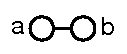
\includegraphics[height=0.4cm]{graph3.pdf}}) with 
vertex labelling with $\pmb{\ell}_{v_1}=a$ and $\pmb{\ell}_{v_2}=b$. We know from 
Corollary~\ref{cor:augmented} that this architecture is upper bounded by 1-WL, starting
from $\pmb{\ell}^{(1)}$. More precisely, we have that $\pmb{\ell}^{(t)}\sqsubseteq\mathbf{F}^{(t-1)}$ for $t\geq 1$.
Consider $\mathbf{F}^{(0)}:=\left(\begin{smallmatrix}1 & 0\\
0 & 1\end{smallmatrix}\right)$ such that $\mathbf{F}^{(0)}$ is good for $\pmb{\ell}$. We also note that $\pmb{\ell}^{(1)}_{v_1}=(a,\{b\})$ and $\pmb{\ell}^{(1)}_{v_2}=(b,\{a\})$. Hence, 
$\mathbf{F}^{(0)}$ is also good for $\pmb{\ell}^{(1)}$. We next show that there does not exists a
weight matrix $\mathbf{W}^{(0)}$ such that $\pmb{\ell}^{(2)}\equiv \mathbf{F}^{(1)}$. Indeed,
$$
\mathbf{F}^{(1)}:=\sigma\Biggl(\frac{1}{2}\biggl(\begin{pmatrix}0 & 1 \\
1 & 0
\end{pmatrix}+
\begin{pmatrix}
	 1 & 0 \\
0 & 1 \end{pmatrix}\biggl)\mathbf{F}^{(0)}\mathbf{W}^{(0)}\Biggr)
=\sigma(\Biggl(\frac{1}{2}\begin{pmatrix}1 & 1 \\
1 & 1
\end{pmatrix}
\mathbf{F}^{(0)}\mathbf{W}^{(0)}\Biggr)=
\sigma\Biggl(\frac{1}{2}\begin{pmatrix}
1& 1\\
1 & 1\\
\end{pmatrix}\mathbf{W}^{(0)}\Biggr).
$$
Hence, independent of the choice of $\mathbf{W}^{(0)}$, both vertices will be assigned the same
feature vector. By contrast, $\pmb{\ell}^{(2)}\sqsubseteq\pmb{\ell}^{(1)}$ and hence
$\pmb{\ell}^{(2)}$ must assign distinct labels to these vertices, since $\pmb{\ell}^{(1)}$ does so. Hence, $\mathbf{F}^{(2)}\not\equiv\pmb{\ell}^{(2)}$.\qed
\end{example}
The example shows that the upper bound for the augmented adjacency architecture as given in Corollary~\ref{cor:augmented} cannot be matched with a lower bound.
In fact the same example can be used to show that the augmented random walk architecture is not as strong as 1-WL, starting from $\pmb{\ell}^{(0)}$. That is the upper bound from Corollary~\ref{cor:augrw1wl} cannot be matched with a lower bound.

In the proof of  Lemma~\ref{lem:findingp} it is also important that $p\neq 0$. THe following simple example shows that the adjacency, random walk and and normalised adjacency architectures are not as strong as 1-WL (recall that for these architectures $p=0$).

\begin{example}\label{example:piszero}
consider the  adjacency architecture on input graph  $(G,\pmb{\ell})$
(\raisebox{-0.4ex}{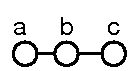
\includegraphics[height=0.5cm]{graph4.pdf}}) with 
vertex labelling with $\pmb{\ell}_{v_1}=a$, $\pmb{\ell}_{v_2}=b$ and $\pmb{\ell}_{v_3}=c$.
Consider $\mathbf{F}^{(0)}:=\left(\begin{smallmatrix}1 & 0 & 0\\
0 & 1 & 0\\
0 & 0 & 1\end{smallmatrix}\right)$ such that $\mathbf{F}^{(0)}$ is good for $\pmb{\ell}$.
Then,
$$
\mathbf{F}^{(1)}:=\sigma\Biggl(\begin{pmatrix}0 & 1 & 0 \\
1 & 0 & 1\\
0 & 1 & 0
\end{pmatrix}\mathbf{F}^{(0)}\mathbf{W}^{(0)}\Biggr)
=\sigma(\mathbf{W}^{(0)}\Biggr)=
\sigma\Biggl(\begin{pmatrix}0 & 1 & 0 \\
1 & 0 & 1\\
0 & 1 & 0
\end{pmatrix}\mathbf{W}^{(0)}\Biggr).
$$
Hence, independent of the choice of $\mathbf{W}^{(0)}$,  vertices $v_1$ and $v_3$ will be assigned the same
feature vector. By contrast, $\pmb{\ell}^{(1)}_{v_1}=(a,\{b\})\neq \pmb{\ell}^{(1)}_{v_2}=(c,\{b\})$.
This example also works for the random walk and and normalised adjacency architectures. \qed
\end{example}

We thus see that having $0<p<1$ is a necessary condition for GNN architectures~(\ref{eq:architecture})
to be as strong as 1-WL.

\subsection{Separating examples}

\openprob{Can we argue, based on results so far how to separate the different GNN models.}
\begin{itemize}
	\item I believe we can use the strongness results do so between the architectures in each group in Table~\ref{tbl:strongGNN}.
	\item It would be great if we can separate all GNNs, even within a group in  Table~\ref{tbl:strongGNN}. Perhaps using $\hat{\pmb{\ell}}$. Also, can one GNN architecture simulate another one? That is, can one find learnable parameters of one model to simulate another one (this is an extension of WL strongness where WL is replaced by the labeling computer by another GNN architecture.) This makes only sense when both GNN architecture are known to be bounded in the same way.
\end{itemize}


\subsection{Bias}
\floris{Perhaps too ambitious...}
\openprob{Can we find examples that show that the bias is needed, i.e., $q\neq 0$ is necessary in general? Note we only need to look at GNN architectures for which $0<p<1$.}
Consider  GNN architectures 
$$\mathbf{F}^{(t+1)}:=\sigma(\mathbf{L}(\mathbf{A}+p\mathbf{I})\mathbf{R}\mathbf{F}^{(t)}\mathbf{W}^{t}),	
$$
with $0<p<1$. We next show that bias is needed.

\begin{example}
	Consider the relaxed augmented random walk architecture
$$\mathbf{F}^{(t+1)}:=\text{sgn}(\tilde{\mathbf{D}}^{-1/2}(\mathbf{A}+p\mathbf{I})\mathbf{F}^{(t)}\mathbf{W}^{t}),
$$
with $0<p<1$. We know that it is upper bounded by 1-WL, starting from $\pmb{\ell}$. We next show that without bias, we cannot get a matching lower bound. Note that this example uses sgn as activation function.

Consider the graph  $(G,\pmb{\ell})$
(\raisebox{-0.4ex}{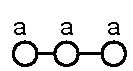
\includegraphics[height=0.5cm]{graph5.pdf}}) with $\pmb{\ell}_{v_1}=\pmb{\ell}_{v_2}=\pmb{\ell}_{v_3}=a$. Let $\mathbf{F}^{(0)}:=\left(\begin{smallmatrix} 1\\1\\1\end{smallmatrix}\right)$.
We have 
$$
\mathbf{F}^{(1)}:=\text{sgn}\Biggl(
\begin{pmatrix}
1/\sqrt{2} & 0 & 0\\
0 & 1/\sqrt{3} & 0\\
0 & 0 & 1/\sqrt{2}
\end{pmatrix}
\begin{pmatrix}
p & 1 & 0\\
1 & p & 1\\
0 & 1 & p
\end{pmatrix}
\begin{pmatrix}
	1\\
	1\\
	1
	\end{pmatrix}\mathbf{W}^{(0)}\Biggr)
=\text{sgn}\Biggl(
\begin{pmatrix}
\frac{1}{\sqrt{2}}(1+p)\\
\frac{1}{\sqrt{3}}(2+p)\\
\frac{1}{\sqrt{2}}(1+p)\end{pmatrix}
\mathbf{W}^{(0)}
\Biggr)
$$
We remark that $\mathbf{W}^{(0)}$ is a $1\times f$-matrix. Clearly, all entries in
$\mathbf{F}^{(1)}$ will have the same sign. By contrast, $\pmb{\ell}^{(1)}_{v_1}=(a,\{a\})\neq
(a,\{a,a\})=\pmb{\ell}^{(1)}_{v_2}$. So, $\pmb{\ell}^{(1)}\not\equiv\mathbf{F}^{(1)}$ for any choice of $\mathbf{W}^{(0)}$.\qed
\end{example}

% \begin{corollary}
% Suppose that $\pmb{\ell}\not\equiv\hat{\pmb{\ell}}$ but $\pmb{\ell}^{(1)}\sqsubseteq \hat{\pmb{\ell}}$. Then, the architecture is bounded by 1-WL, starting from $\pmb{\ell}^{(1)}$.
% \end{corollary}
% \begin{proof}
% Let $t=0$. We have that $\pmb{\ell}^{(1)}\sqsubseteq \pmb{\ell}\sqsubset \mathbf{F}^{(0)}$. For $t=1$, assume that $\pmb{\ell}^{(2)}_v=\pmb{\ell}^{(2)}_w$. We show that
% $\mathbf{F}_{v\bullet}^{(1)}=\mathbf{F}_{w\bullet}^{(1)}$.
% Indeed, we have that $\pmb{\ell}^{(1)}_v=\pmb{\ell}^{(1)}_w$ and
%  for every $u\in N_G(v)$ and corresponding $u'\in N_G(w)$,
%  $\pmb{\ell}^{(1)}_u=\pmb{\ell}^{(1)}_{u'}$. Then,
%  $\pmb{\ell}^{(1)}\sqsubseteq \hat{\pmb{\ell}}$ implies that
%   $\mathbf{L}_{vv}=\mathbf{L}_{ww}$, $\mathbf{R}_{vv}=\mathbf{R}_{ww}$ and
% $\mathbf{B}_{v\bullet}=\mathbf{B}_{w\bullet}$.
% Furthermore, for every $u\in N_G(v)$ and corresponding $u'\in N_G(w)$, $\mathbf{R}_{uu}=\mathbf{R}_{u'u'}$. By induction, also $\pmb{\ell}^{(1)}\subseteq \mathbf{F}^{(0)}$. This suffices to conclude that $\mathbf{F}^{(1)}_{v\bullet}=\mathbf{F}^{(1)}_{w\bullet}$. For $t>2$, assume that $\pmb{\ell}^{(t)}_v=\pmb{\ell}^{(t)}_w$. Then,
%  $\pmb{\ell}^{(t-1)}_v=\pmb{\ell}^{(t-1)}_w$ and for every $u\in N_G(v)$ and corresponding $u'\in N_G(w)$,  $\pmb{\ell}^{(t-1)}_u=\pmb{\ell}^{(t-1)}_{u'}$. In particular,
%  since $\pmb{\ell}^{(t-1)}\sqsubseteq \pmb{\ell}^{(1)}$,
%  $\pmb{\ell}^{(1)}_v=\pmb{\ell}^{(1)}_w$ and for every $u\in N_G(v)$ and corresponding $u'\in N_G(w)$,  $\pmb{\ell}^{(1)}_u=\pmb{\ell}^{(1)}_{u'}$. Using that $\pmb{\ell}^{(1)}\sqsubseteq \hat{\pmb{\ell}}$ holds, this implies that
%  $\mathbf{L}_{vv}=\mathbf{L}_{ww}$, $\mathbf{R}_{vv}=\mathbf{R}_{ww}$ and
% $\mathbf{B}_{v\bullet}=\mathbf{B}_{w\bullet}$. Furthermore, for every $u\in N_G(v)$ and corresponding $u'\in N_G(w)$, $\mathbf{R}_{uu}=\mathbf{R}_{u'u'}$. By induction, also $\pmb{\ell}^{(t-1)}\subseteq \mathbf{F}^{(t-2)}$. This suffices to conclude that $\mathbf{F}^{(t-1)}_{v\bullet}=\mathbf{F}^{(t-1)}_{w\bullet}$.
% \end{proof}
% This corollary applies, for example, for the normalized adjacency and augmented adjacency architecture.

%
% \todo{From an upper bound perspective, $\mathbf{L}$ has no apparent impact when it is degree related. By contrast, $\mathbf{R}$ speeds up
% 1-WL with one step. The role of $p$ and $q$ and $\mathbf{B}$ also do seem to have an impact for upper bounds. Can we say something more here?}
%!TEX root = quiver.tex

%!TEX root =main.tex
\section{GNNs without self}
\floris{The following needs to be developed in more detail.}
\floris{The idea in this section is to reconsider GNNs without $\mathbf{I}$. The lower bound proof shows that having $\mathbf{I}$ is required to encode the labels of the vertices themselves. So, when absent, we should be able to upper and lower bound using a variation of WL in which only neighbor labels are accounted for. In some sense, this is a generalization of the unlabeled case by~\cite{grohewl} but lifted to labeled graphs. It will allow us to seperate some  more architectures.}

We have seen in Example~\ref{example:piszero} that GNN architectures in which $p=0$ are not necessarily WL-strong, starting from $\hat{\pmb{\ell}}$. Intuitively, the reason is that when $p=0$, the only features that are propagated relate to neighborhoods of vertices and not the features of the vertices themselves. In this section we investigate the expressive power of architectures of the form:
\begin{equation}
\mathbf{F}^{(t)}:=\sigma\left(\mathbf{L}\mathbf{A}\mathbf{R}\mathbf{F}^{(t-1)}\mathbf{W}^{(t-1)} + q\mathbf{J}\right). \label{eq:architecture_noid}
\end{equation}
In a nutshell, we will upper and lower bound such architectures by 
 considering a \textit{weaker variant of WL}  which only takes neighborhood information into account.
 %  Indeed,
% in GNN architectures of the form~\ref{eq:architecture_noid}, the absence of the identity has a consequence that features are updated based on adjacency information alone. We make this now more precise.

We define the \textit{neighbor-only WL}, NWL for short, process as follows. Let $G=(V,\pmb{\mu})$ be a labeled graph and let $\Sigma$ be a set of labels. Initially, let $\pmb{\mu}^{(0)}:=\pmb{\mu}$. 
Then, the NWL procedure computes a labeling $\pmb{\mu}^{(t)}$, for $t> 0$, as follows: 
$$
\pmb{\mu}^{(t)}_v:=\textsc{Hash}\bigl(\ldbl \pmb{\mu}_u^{(t-1)} \st u \in N_G(v) \rdbl\bigr),
$$
where $\textsc{Hash}$ bijectively maps the multi-set $\ldbl \pmb{\mu}_u^{(t-1)} \st u \in N_G(v) \rdbl$ of labels of $v$'s neighbors to a unique label in $\Sigma$, which has not been used in previous iterations. When the number of distinct labels in $\pmb{\mu}^{(t)}$ and $\pmb{\mu}^{(t-1)}$ is the same, the NWL algorithm terminates.
Termination is guaranteed in at most $n$ steps. We refer to the resulting labeling as the \textit{NWL labeling of $(G,\pmb{\mu})$}. 

As before, given matrices $\mathbf{L}$ and $\mathbf{R}$ we define the set of 
extended labels as $\hat{\Sigma}=\Sigma\cup (\Sigma\times L\times R)$ with
$L:=\{\mathbf{L}_{vv}\mid v\in V\}$ and $R:=\{\mathbf{R}_{vv}\mid v\in V\}$.
The following counterpart of Theorem~\ref{thm:generalbound} is now easily verified.

\begin{theorem}\label{thm:generalbound_noid}
GNN architectures of the form~(\ref{eq:architecture_noid}) for which 
$\pmb{\mu}^{(1)}\sqsubseteq \hat{\pmb{\mu}}$ holds for any labeled graph $(G,\pmb{\mu})$, are bounded by NWL on $(G,\hat{\pmb{\ell}})$.
\end{theorem}
Compared to Theorem~\ref{thm:generalbound} the extra condition involving $\pmb{\mu}^{(1)}\sqsubseteq \hat{\pmb{\mu}}$ is needed to ensure that the values in $\mathbf{L}$ are functionally determined by degree information of the vertices.

\begin{proof}
We show the upper bound by NWL by induction on the number of iterations. For $t=0$, we have, by assumption, that 
$\pmb{\ell}\sqsubseteq \mathbf{F}^{(0)}$. Clearly,
$\hat{\pmb{\mu}}{}^{(0)}\sqsubseteq \pmb{\ell}$ and hence also 
$\hat{\pmb{\mu}}{}^{(0)}\sqsubseteq\mathbf{F}^{(0)}$. We next assume that the induction hypothesis holds for $t\geq 0$ and consider $t+1$. We need to show that 
$\hat{\pmb{\mu}}{}^{(t+1)}_v=\hat{\pmb{\mu}}{}^{(t+1)}_w$ implies that $\mathbf{F}^{(t+1)}_{v\bullet}=\mathbf{F}^{(t+1)}_{w\bullet}$. By definition,
$\hat{\pmb{\mu}}{}^{(t+1)}_v=\hat{\pmb{\mu}}{}^{(t+1)}_w$ implies
$$
\ldbl \hat{\pmb{\mu}}{}^{(t)}_u \st u \in N_G(v) \rdbl=
 \ldbl \hat{\pmb{\mu}}{}^{(t)}_u \st u \in N_G(w) \rdbl.$$
 Since $\hat{\pmb{\mu}}{}^{(t)}\sqsubseteq \hat{\pmb{\mu}}{}^{(t-1)}\sqsubseteq \cdots\sqsubseteq \hat{\pmb{\mu}}{}^{(0)}$, this implies that  there is a bijection $b:N_G(v)\to N_G(w):u\mapsto u'$ such that $\hat{\pmb{\mu}}{}^{(t)}_u=\hat{\pmb{\mu}}{}^{(t)}_{u'}$ and hence also 
 $\hat{\pmb{\mu}}{}^{(0)}_u=\hat{\pmb{\mu}}{}^{(0)}_{u'}$.
From the definition of $\hat{\pmb{\mu}}{}^{(0)}$, this implies that for every $u\in N_G(v)$ and corresponding $u'\in N_G(w)$, $\mathbf{L}_{uu}=\mathbf{L}_{u'u'}$ and $\mathbf{R}_{uu}=\mathbf{R}_{u'u'}$. By the assumption that on $\mathbf{L}$ we further have that
$\mathbf{L}_{vv}=\mathbf{L}_{ww}$.
By the induction hypothesis we also for every $u\in N_G(v)$
   and corresponding $u'\in N_G(w)$, $\mathbf{F}^{(t)}_{u\bullet}=\mathbf{F}^{(t)}_{u'\bullet}$. It now suffices to observe that
  \begin{align*}
	  \mathbf{F}^{(t+1)}_{v\bullet}&=\sigma\Biggl(\mathbf{L}_{vv}\Bigl(\sum_{u\in N_G(v)} \mathbf{R}_{uu}\mathbf{F}^{(t)}_{u\bullet}\Bigr)\mathbf{W}^{(t)}+ q\mathbf{J}_{v\bullet}\Biggr)\\
	 & =\sigma\Biggl(\mathbf{L}_{ww}\Bigl(\!\!\sum_{u'\in N_G(w)}\!\! \mathbf{R}_{u'u'}\mathbf{F}^{(t)}_{u'\bullet}\Bigr)\mathbf{W}^{(t)}+ q\mathbf{J}_{w\bullet}\Biggr)\\
	  &=\mathbf{F}^{(t+1)}_{w\bullet},
\end{align*}
as desired.
\end{proof}

We can also show that GNN architectures of the form~(\ref{eq:architecture_noid}) 
are NWL-strong, starting from $\hat{\pmb{\mu}}$.
\begin{proposition}
The class of GNN architectures of the form~(\ref{eq:architecture_noid}) for which 
	$\pmb{\mu}^{(1)}\sqsubseteq \hat{\pmb{\mu}}$ holds for any labeled graph $(G,\pmb{\mu})$, are NWL-strong, starting from $\hat{\pmb{\mu}}$.
\end{proposition}
\begin{proof}
We closely follow the proof of Theorem~\ref{thm:lowerb_general}.
 By assumption, $\mathbf{F}^{(0)}\equiv \hat{\pmb{\mu}}$ and $\mathbf{F}^{(0)}$
 row independent modulo equality. Consider $t>0$ and assume that $\mathbf{F}^{(t-1)}$ is good for $\hat{\pmb{\mu}}$. It is easily verified that the proof of Lemma~\ref{lem:rightgood} also works here. Hence, $\mathbf{R}\mathbf{F}^{(t-1)}$ is also good for  $\hat{\pmb{\mu}}$. We can also use first part of the proof of Lemma~\ref{lem:findingp}. Using the notation in that proof, we know that there exists a matrix $M^{(t-1)}$ such that for every $v\in V$ and $c\in\Sigma^{(t-1)}$:
 $$
 (\mathbf{A}\mathbf{R}\mathbf{F}^{(t-1)}\mathbf{M}^{(t-1)})_{vc}=|u\in N_G(v)| \mathbf{R}\mathbf{F}_{u\bullet}^{(t-1)}\sim c\}|
 $$

\floris{To be worked out further.... }
\end{proof}

Clearly, the two architectures without $\mathbf{I}$, RW-GNN and NA-GNN satisfy the conditions in the Theorem. The same holds for the following architecture:
\begin{description}
 \item[\textit{Adjacency} (A-GNN):]
% $\mathbf{L}=\mathbf{R}:=\mathbf{I}$, $p=q:=0$. Hence,
$
\mathbf{F}^{(t)}:=\sigma\left(\mathbf{A}\mathbf{F}^{(t-1)}\mathbf{W}^{(t)}\right)
$
\end{description}
which was shown to be bounded by WL and WL-strong on unlabeled graphs in ~\cite{grohewl}.
\floris{We need to make the connection with the unlabelled case more precise.}

\subsection{Special cases}
\openprob{All what follows needs to be shown (if we want ;-)}
\begin{corollary}
The A-GNN,  NA-GNN  and RW-GNN architectures are bounded by WWL, starting from $(G,\pmb{\mu})$.	
\end{corollary}
Since $\hat{\pmb{\ell}}{}^{(k)}\sqsubseteq \hat{\pmb{\mu}}{}^{(k)}$, this corollary provides a stronger upper bound than Corollary. Indeed, it says that these architecture cannot classify vertices in a finer way than the weak version of WL. 

We can again zoom in on these three architectures and show that these architecture can be bounded by
$\pmb{\mu}^{(t)}$ rather than $\hat{\pmb{\mu}}^{(t)}$. 
\begin{corollary}
The A-GNN  and RW-GNN architectures are bounded by WWL, starting from $(G,\pmb{\ell})$.
The NA-GNN architecture is bounded by WWL, starting from $(G,\pmb{\mu}{}^{(1)})$.
\end{corollary}

\subsection{Lower bounds}

\openprob{We can tell, I believe, the same story as before but now for WWL. It should allow us to separate classes with $\mathbf{I}$.}




\bibliographystyle{apalike}
\bibliography{refs}

% \section{Introduction}
\begin{itemize}
  \item After going through Kipf's code, I did not find any sign of bias being
    used in the activation-function calls. In fact, it seems to me that they
    explicitly set it to 0 (see 
    https://github.com/tkipf/gcn).
    \item Interestingly, in~\cite{xhlj19} they claim to have shown Kipf's
      architecture is strictly less powerful than the 1-WL algorithm!
      (However, in his website, Kipf observes that they assume ``mean
      pooling''.)
   \item In~\cite{Wu2019}, it is said "We hypothesize that the nonlinearity
     between GCN layers is not critical - but that the majority of the
     benefit arises from the local averaging." This worth making more
     precise or even invalidate it theoretically.
   \item In~\cite{hyl17} they have a paragraph on Relation to the Weisfeiler-Lehman
     Isomorphism Test which makes more sense than Kipf. They clarify that
     isomorphism is not the end goal!
\end{itemize}

\section{Preliminaries}
Let $M = \ldbl m_0, m_1, \dots \rdbl$ denote a \emph{multiset} and $M(x)$
stand for the \emph{multiplicity} of the element $x$ within $M$.

\paragraph{Graphs.}
An \emph{(undirected) graph} $G$ is a pair $(V,E)$ where $V$ is a finite set
of \emph{vertices} and $E \subseteq \{\{u,v\} \st (u,v) \in V \times V, u \neq
v\}$ is a finite set of \emph{edges}. Let $V(G)$ and $E(G)$ denote the set of
vertices and edges of $G$ respectively. Let $N_G(u)$ denote the
\emph{neighbourhood} of vertex $u$ in $G$. That is to say, $N_G(u) := \{v \in V(G)
\st \{u,v\} \in E(G)\}$.

We will mostly work with the \emph{adjacency matrix} $\mathbf{A}$ of the
graph $G$. That is, $\mathbf{A}$ is the square $|V(G)| \times |V(G)|$ matrix
such that the entry $\mathbf{A}_{ij}$ is $1$ if $\{i,j\} \in E(G)$ and $0$
otherwise.

A \emph{vertex labelling} is a function $\ell: V(G) \to \Lambda$ with an
arbitrary co-domain $\Lambda$ of \emph{labels} and a \emph{labelled
graph} is a pair $(G,\ell)$ where $G$ is a graph and $\ell : V(G) \to \Lambda$
is a vertex-labelling function. A \emph{label class} $Q \subseteq V(G)$, with
respect to a vertex labelling $\ell$, is a maximal subset of $V(G)$ such that
$\ell(u) = \ell(v)$ for all $u,v \in Q$.

Let $\ell,\ell' : V(G) \to \Lambda$ be vertex labellings.
We say that $\ell$ \emph{refines} $\ell'$, written $\ell \sqsubseteq \ell'$,
if and only if for all $u,v \in V(G)$ we have
\[
    \ell(u) = \ell(v) \implies \ell'(u) = \ell'(v).
\]
Furthermore, we say that $\ell$ and $\ell'$ are \emph{equivalent}, written
$\ell \equiv \ell'$, if and only if $\ell \sqsubseteq \ell'$
and $\ell' \sqsubseteq \ell$. 

\todo{F. We should clarity what an unlabeled graph is.}
\paragraph{Isomorphism.}
We say two labelled graphs $(G,\ell_G)$ and $(H,\ell_H)$ are \emph{isomorphic}
if there exists an edge-preserving label-consistent bijection $\beta : V(G)
\to V(H)$. That is, $\beta$ is such that 
\begin{itemize}
    \item $\{u,v\} \in E(G)$ if and only if $\{\beta(u),\beta(v)\} \in E(H)$ and
    \item $\ell_G(u) = \ell_G(v)$
      if and only if $\ell_H(\beta(u)) = \ell_H(\beta(v))$.
\end{itemize}



\subsection{The Weisfeiler-Leman algorithm}
Let $(G,\ell)$ be a labelled graph. The $1$-WL algorithm computes, in each
iteration $t \geq 0$, a vertex labelling $\ell^{(t)} : V(G) \to \Lambda$ which
depends on the labelling from the previous iteration. Initially, we set
$\ell^{(0)} := \ell$. For $t > 0$ we set
\[
   \ell^{(t)}(u) := 
    \hash\left(\ell^{(t-1)}(u), \ldbl \ell^{(t-1)}(v) \st v \in N_G(u) \rdbl\right)
\]
where $\hash$ bijectively maps pairs of labels and label-multisets to a label
from $\Lambda$.  The algorithm terminates when a \emph{stable labelling} is
reached, i.e. when $\ell^{(t+1)} \equiv \ell^{(t)}$. Observe that
$\ell^{(t+1)} \sqsubseteq \ell^{(t)}$ for all $t \geq 0$ and that termination
is therefore guaranteed after at most $|V(G)|$ iterations.

\paragraph{Isomorphism heuristic.} 
If the stable labellings of two labelled graphs $(G,\ell_G)$ and $(H,\ell_H)$
have a different number of vertices labelled $\lambda$, for some label
$\lambda \in \Lambda$, the algorithm correctly concludes that they are not
isomorphic.

\subsection{Graph neural networks}
Consider a labelled graph $(G,\ell)$ with $\ell : V(G) \to \mathbb{R}^{1
\times a_0}$.  This, intuitively, means that every vertex $v$ is annotated
with a \emph{feature vector} $\ell(v) \in \mathbb{R}^{1 \times a_0}$.

A graph neural network (GNN, for short) is composed of layers which aggregate
the labels of the neighbours of a vertex, as computed by the previous layer,
and feed this aggregated information to the next layer.  A basic GNN model can
be implemented by setting $f^{(0)} := \ell$ and having each layer $t \geq 0$
compute a new feature vector $f^{(t+1)}(v) \in \mathbb{R}^{1 \times a_{t+1}}$ as
follows
\[
  \sigma\left(
    f^{(t)}(v) \mathbf{W}_1^{(t)} +
    \sum_{w \in N_G(v)} f^{(t)}(w) \mathbf{W}_2^{(t)}
  \right)
\]
where $\mathbf{W}_1^{(t)}, \mathbf{W}_2^{(t)} \in \mathbb{R}^{a_t \times
a_{t+1}}$ are parameter matrices and $\sigma$ denotes a non-linear activation
function such as the rectified linear unit (ReLU for short).\footnote{For ease
of comparison with the work of Kipf and Welling~\shortcite{kipf-loose} we do
not use a \emph{bias}.}
Note that the feature-vector update can be re-written in matrix
form as
\begin{equation}\label{eqn:gnn}
  \mathbf{F}^{(t+1)} = \sigma\left(
    \mathbf{F}^{(t)}\mathbf{W}_1^{(t)} +
    \mathbf{AF}^{(t)}\mathbf{W}_2^{(t)}
  \right)
\end{equation}
where $\mathbf{F}^{(t)}$ is the $|V(G)| \times a_t$ matrix such that $i$th row 
$\mathbf{F}^{(t)}_{i\bullet}$ of  $\mathbf{F}^{(t)}$ is the row vector $f^{(t)}(i)$ and $\mathbf{A}$ is the
adjacency matrix of $G$.

\subsubsection{GNNs are Weisfeiler-Leman powerful}
It has been shown that GNNs are as powerful as the $1$-WL
algorithm~\cite{grohewl}, a formal statement follows. For a labelled graph
$(G, \ell)$, let us write $\ell \equiv \lambda$ if $\ell$ maps every vertex of
$G$ to the same label $\lambda$.
\begin{proposition}[Corollary 12 from~\cite{grohewl}]\label{pro:grohe}
  Let $(G,\ell)$ be a labelled graph such that $\ell \equiv \lambda$. Then
  there exists a sequence of matrices such that for all $t \in \mathbb{N}$ and
  for $f^{(t)}$, as defined by Equation~\eqref{eqn:gnn} with $f^{(0)} = \ell$
  and $\sigma$ being ReLU, we have $f^{(t)} \equiv \ell^{(t)}$.
\end{proposition}
\todo{F. What is the $\lambda$ here?}

\subsection{GNNs and Kipf and Welling}
In~\cite{kipf-loose}, the following notion of GNNs was proposed.
Let $\mathbf{D}$ be the \emph{degree matrix} of $G$, that is $\mathbf{D}$
is the diagonal matrix such that $
    \mathbf{D}_{ii} = |N_G(i)|$,
 and the feature update rule used has the following form:
\begin{equation}\label{eqn:kipf-update}
    \mathbf{F}^{(t+1)} = \sigma\left(
        \mathbf{D}^{-1/2}\mathbf{A}\mathbf{D}^{-1/2}
        \mathbf{F}^{(t)}\mathbf{W}^{(t)}
    \right),
\end{equation}
where $\mathbf{D}^{-1/2}$
is the diagonal matrix with
$\mathbf{D}^{-1/2}_{ii} =
\frac{1}{\sqrt{\mathbf{D}_{ii}}}$. Compared with~(\ref{eqn:gnn}) this
is simpler update rule. It is remarked in~\cite{kipf-loose} that this update
rule is ``loosely speaking'' 1-WL. In this paper, we want to make this connection 
precise. More precisely, we show that
\begin{theorem}\label{pro:grohe}
  Let $(G,\ell)$ be a labelled graph. Then there exists a sequence of matrices such that for all $t \in \mathbb{N}$ and
  for $f^{(t)}$, as defined by Equation~\eqref{eqn:kipf-update} with $f^{(0)} = \ell$
  and $\sigma$ being ReLU, we have $f^{(t)} \equiv \ell^{(t)}$.
\end{theorem}
In other words, the GNNs by Kipf and Welling are as powerful as 1-WL.
\todo{F. Can we say anything about the upper bound of their expressive power.
I guess this follows from Grohe's paper?}

\subsection{Assumptions}
For notational convenience, we assume that all vertices have a non-empty
neighbourhood. This can be achieved, for instance, by introducing a new
vertex with a fresh new label and connecting all vertices without neighbours
to it.

\section{A linear-update architecture for unlabelled graphs}
Our first result is to ``simplify'' Proposition~\ref{pro:grohe} by simulating
their affine-update architecture using a linear update instead thus allowing
us to work with a single parameter matrix---at the price of having to extend
the feature vectors. We state below the formal claim.

\subsection{Look ma, one matrix}
Let us re-define the basic GNN we deal with. In each
layer $t \geq 0$, we compute a new feature vector
\[
    f^{(t+1)}(v) = \sigma\left(
        \sum_{w \in N_G(v)} f^{(t)}(w) \mathbf{W}^{(t)}
    \right)
\]
in $\mathbb{R}^{1 \times a_{t+1}}$ for $u$ where $\mathbf{W}^{(t)}$ is a
parameter matrix from $\mathbb{R}^{a_t \times a_{t+1}}$ and $\sigma$
is the ReLU activation function. Once more, we work with the matrix
form of the update:
\begin{equation}\label{eqn:gnn-linear}
    \mathbf{F}^{(t+1)} = \sigma\left(\mathbf{AF}^{(t)}\mathbf{W}^{(t)}\right).
\end{equation}

We will show that, if we set $f^{(t)}(v) := (\ell(v), 1)$ for all vertices
$v$, then GNNs with this architecture are also as
powerful as the $1$-WL algorithm.

\begin{proposition}
  Let $(G,\ell)$ be a labelled graph such that $\ell \equiv \lambda$. Then
  there exists a sequence of matrices such that for all $t \in \mathbb{N}$ and
  for $f^{(t)}$, as defined by Equation~\eqref{eqn:gnn-linear} with
  $f^{(0)}(v) = (\lambda, 1)$, for all $v \in V(G)$, and $\sigma$ being ReLU,
  we have $f^{(t)} \equiv \ell^{(t)}$.
\end{proposition}

\todo{G: I am up to here with cleaning a bit}

As a starting point, we re-establish Lemma 9
from~\cite{grohewl} for the ReLU function.
\begin{lemma}
  Let
  $\mathbf{B}\in \Nb^{s\times t}$ be a matrix in which all
  rows are pairwise disjoint (and no row consists entirely
  out of zeroes\footnote{I believe that this can be
  guaranteed in 1-WL}).\todo{G: with our extended features we actually guarantee this for free by adding the 1 column; also, t as dimension is a bad choice\ldots}
  Then there exists a matrix $\mathbf{X}$ and a constant $m$
  such that $\textsf{ReLU}(\mathbf{BX}-m\mathbf{J})$ is
  non-singular.
\end{lemma}
\begin{proof}
Let $M$ be the maximal entry in $\mathbf{B}$ and consider the column vector $\mathbf{z}=(1,M,M^2,\ldots,M^{t-1})^{\textsc{t}}$.
Then each entry in $\mathbf{b}=\mathbf{B}\mathbf{z}$ is positive and they are all pairwise distinct. Assume that $\mathbf{b}=(b_1,b_2,\ldots,b_t)^{\textsc{t}}\in\Rb^{s\times 1}$
such that $0< b_1< b_2<\cdots < b_s$. Consider the row vector $\mathbf{x}=\left(\frac{1}{b_1},\ldots,\frac{1}{b_s}\right)\in \Rb^{1\times s}$. Then, for $\mathbf{C}=\mathbf{b}\mathbf{x}$
$$
(\mathbf{C})_{ij}=\frac{b_i}{b_j}  \text{ and } (\mathbf{C})_{ij}=\begin{cases}  1 & \text{if $i=j$}\\
< 1 & \text{if $i<j$}\\
> 1 & \text{if $i>j$}.
\end{cases}
$$
Let $m$ be the greatest value  in $\mathbf{C}$ smaller than $1$.
% G: I think the m instantiated here is not correct
%, i.e., $m=\frac{b_s}{b_1}$.
Consider $\mathbf{D}=\mathbf{C}- m\mathbf{J}$.
Then,
$$
\mathbf{D}_{ij}=\frac{b_i}{b_j}- m \text{ and } (\mathbf{D})_{ij}=\begin{cases}  1-m & \text{if $i=j$} \\
\leq 0 & \text{if $i<j$}\\
>0  & \text{if $i>j$}.
\end{cases}
$$
As a consequence,
$$
\textsf{ReLU}(\mathbf{D})_{ij}=\begin{cases}  1-m & \text{if $i=j$}\\
0 & \text{if $i<j$}\\
>0  & \text{if $i>j$}.
\end{cases}
$$
This is an upper triangular matrix with (nonzero) value $1-m$ on its diagonal. It is therefore non-singular. So, the lemma is satisfied by taking $m$ as above and
%$m=b_s/b_1$ and % G: this still looks wrong
$\mathbf{X}=\mathbf{z}\mathbf{x}$.
\end{proof}

It is now easy to see that we can define weight matrices such that
\[
    \mathbf{F}^{(t+1)} = \textsf{ReLU}\left(\mathbf{AF}^{(t)}\mathbf{W}^{(t)}-m^{(t)}\mathbf{J}\right).
\]
is again equivalent to $c_\ell^{(t+1)}$.  We show that we modify $\mathbf{F}^{(t)}$ and $\mathbf{W}^{(t)}$
such that can rewrite the update rule in Kipf form.

Let $\mathbf{d}^{(t)}:=\mathbf{A}^{t}\mathbf{1}^\textsc{t}$. That is, $\mathbf{d}^{(t)}_v$ counts the paths from vertex $v$ of length $t$. We note that for undirected graphs $\mathbf{d}^{(t)}$ holds non-negative entries\footnote{For directed graphs, we may consider $I+A$ instead.}
We now use a similar construction of $\mathbf{W'}^{(t)}$ in the proof of Theorem~\ref{thm:simpler-grohe}, i.e.,
\[
\mathbf{W'}^{(t)}=\begin{pmatrix}
\mathbf{W}^{(t)} & \mathbf{0}_{d\times 1}\\
\left(-\frac{m^{(t)}}{d_1^{(t+1)}},\ldots,-\frac{m^{(t)}}{d_n^{(t+1)}}\right) & 1
\end{pmatrix}.
\]
and we replace $\mathbf{F}$ by $\mathbf{F'}=[\mathbf{F},\mathbf{1}]$. Then,
\begin{align}
    \mathbf{F'}^{(t+1)} 
        &=\textsf{ReLU}(\mathbf{A}\mathbf{F'}\mathbf{W'}^{(t)}) \nonumber \\
        &=[\textsf{ReLU}(\mathbf{A}\mathbf{F}^{(t)}\mathbf{W}^{(t)}-m^{(t)}\mathbf{J}),\textsf{ReLU}(\mathbf{d}^{(t+1)})]. \nonumber \\
        &=[\mathbf{F}^{(t+1)}, \mathbf{d}^{(t+1)}] \label{eq:Fc}
\end{align}
It now suffices to show that $\mathbf{F'}^{(t)}$ is equivalent to $c_\ell^{(t)}$. Since $\mathbf{F}^{(t)} \equiv c_\ell^{(t)}$ and by~\eqref{eq:Fc} $\mathbf{F'}^{(t+1)} \sqsubseteq \mathbf{F}^{(t+1)}$ it suffices to prove that $c_\ell^{(t)} \sqsubseteq \mathbf{F'}^{(t)}$.
This boils down to the following lemma.

\begin{lemma}\label{lem:deg-in-WL}
    Let $(G,c)$ be a labeled graph.
    Then for all $t \geq 0$ we have that 
    $c_\ell^{(t)} \sqsubseteq \mathbf{d}^{(t)}$. \filip{I think it's a bit ugly that $c$ is a function and $d$ is a vector but I find this statement better. Maybe we should define $c$ in bold (as a vector)?}
%     \[
%         c^{(t)}(u) = c^{(t)}(v) \implies d^{(t)}_u = d^{(t)}_v.
%     \]
\end{lemma}
\begin{proof}
Since $c_\ell^{(0)}$ assigns every vertex the same label, and $\mathbf{d}^{(0)}=\mathbf{1}^t$, our hypothesis holds for the base case.
%Filip: I started modifying here
For the induction step suppose that $c_\ell^{(t-1)}(v)=c_\ell^{(t-1)}(w)$ implies $\mathbf{d}^{(t-1)}_v=\mathbf{d}^{(t-1)}_w$.
Given a label $c$ we will use the notation $\mathbf{d}^{(t-1)}_c$, which is equal to $\mathbf{d}^{(t-1)}_v$ for any $v$ such that $c_\ell^{(t-1)} = c$. By the induction assumption this definition does not depend on the choice of $v$.

Take two vertices $v$ and $w$ such that $c_\ell^{(t)}(v)=c_\ell^{(t)}(w)$. By definition of the 1-WL algorithm 
$$
|N_G(v)\cap (c_\ell^{(t-1)})^{-1}(c)|=|N_G(w)\cap (c_\ell^{(t-1)})^{-1}(c)|
$$
for any label $c$ in ${\cal C}^{(t-1)}$ (i.e., the image of $c_\ell^{(t-1)}(V)$). Then
\begin{align*}
\mathbf{d}^{(t)}_v&=\sum_{x\in N_G(v)} \mathbf{d}^{(t-1)}_{x}\\
&=\sum_{c\in{\cal C}^{(t-1)}} |N_G(v)\cap (c_\ell^{(t-1)})^{-1}(c)|\mathbf{d}^{(t-1)}_{c}\\
&=\sum_{c\in{\cal C}^{(t-1)}} |N_G(w)\cap (c_\ell^{(t-1)})^{-1}(c)|\mathbf{d}^{(t-1)}_{c}\\
&=\sum_{y\in N_G(w)} \mathbf{d}^{(t-1)}_{y}\\
&=\mathbf{d}^{(t)}_w,
\end{align*}
as required.
%Floris' old stuff
% Suppose that $c_\ell^{(t-1)}(v)=c_\ell^{(t-1)}(w)$ implies that $\mathbf{d}^{(t-1)}_v=\mathbf{d}^{(t-1)}_w$.
% Take two vertices $v$ and $w$ such that $c_\ell^{(t)}(v)=c_\ell^{(t)}(w)$. This implies that for any label $c$ in ${\cal C}^{(t-1)}$ (i.e., the image of $c_\ell^{(t-1)}(V)$), 
% $$|N_G(v)\cap (c_\ell^{(t-1)})^{-1}(c)|=|N_G(w)\cap (c_\ell^{(t-1)})^{-1}(c)|.$$
% By induction, we know that for any two vertices $x$ and $y$ in $N_G(v)\cap (c_\ell^{(t-1)})^{-1}(c)$,
% $\mathbf{d}^{(t-1)}_{x}=\mathbf{d}^{(t-1)}_{y}$. Let us denote by $x_c$ an arbitrary vertex in 
% $N_G(v)\cap (c_\ell^{(t-1)})^{-1}(c)$. Then,
% \begin{align*}
% \mathbf{d}^{(t)}_v&=\sum_{x\in N_G(v)} \mathbf{d}^{(t-1)}_{x}\\
% &=\sum_{c\in{\cal C}^{(t-1)}} |N_G(v)\cap (c_\ell^{(t-1)})^{-1}(c)|\mathbf{d}^{(t-1)}_{x_c}\\
% &=\sum_{c\in{\cal C}^{(t-1)}} |N_G(w)\cap (c_\ell^{(t-1)})^{-1}(c)|\mathbf{d}^{(t-1)}_{x_c}\\
% &=\sum_{c\in{\cal C}^{(t-1)}} |N_G(w)\cap (c_\ell^{(t-1)})^{-1}(c)|\mathbf{d}^{(t-1)}_{y_c}\\
% &=\sum_{y\in N_G(w)} \mathbf{d}^{(t-1)}_{y}\\
% &=\mathbf{d}^{(t)}_w,
% \end{align*}
% where $y_c$ denotes an arbitrary vertex in  $N_G(w)\cap (c_\ell^{(t-1)})^{-1}(c)$ and hence, by induction,
% $\mathbf{d}^{(t-1)}_{x_c}=\mathbf{d}^{(t-1)}_{y_c}$.
\end{proof}

\begin{theorem}\label{thm:denorm-kipf}
    Theorem~\ref{thm:simpler-grohe} holds as well 
    %(modulo, perhaps, additional layers needed) 
    if $\sigma$ is the ReLU
    activation function.
\end{theorem}

\section{Labelled graphs}
\todo{G: we need to argue that what we worked out in the previous section
works for labelled graphs too (even if only for ReLU...)}


\section{Normalized convolutional architecture}
Theorem~\ref{thm:denorm-kipf}
can be seen as a
``denormalized'' version of the update rule introduced
in~\cite{kipf-loose}.

Let $\mathbf{D}$ be the \emph{degree matrix} of $G$, that is $\mathbf{D}$
is the diagonal matrix such that
\[
    \mathbf{D}_{ii} = |N_G(i)|.
\]
In this section we consider the following update rule
\begin{equation}
    \mathbf{H}^{(t+1)} = \sigma\left(
        \mathbf{D}^{-1/2}\mathbf{A}\mathbf{D}^{-1/2}
        \mathbf{H}^{(t)}\mathbf{W}^{(t)}
    \right),
\end{equation}
where $\mathbf{D}^{-1/2}$
is the diagonal matrix with
$\mathbf{D}^{-1/2}_{ii} =
\frac{1}{\sqrt{\mathbf{D}_{ii}}}$.

\subsection{(Right-)half Kipf}
We will repeat the argument leading to Theorem~\ref{thm:denorm-kipf} in order
to prove that we can modify $\mathbf{F}^{(t)}$ and $\mathbf{W}^{(t)}$
such that
\begin{equation}\label{eqn:half-kipf}
    \mathbf{F}^{(t+1)} \equiv
    \mathbf{F'}^{(t+1)} :=
    \textsf{ReLU}\left(\mathbf{AD}^{-1/2}\mathbf{F'}^{(t)}\mathbf{W'}^{(t)}\right).
\end{equation}
Once more, we let $\mathbf{F'}^{(0)} = [\mathbf{F}^{(0)},
\mathbf{1}^\textsc{T}]$. For the weight matrices, we define
\[
    \mathbf{W'}^{(t)}=
    \begin{pmatrix}
        \mathbf{W}^{(t)} & \mathbf{0}_{d\times 1}\\
        \left(
            -\frac{m^{(t)}\sqrt{d_1^{(1)}}}{d_1^{(t+1)}},
            \ldots,
            -\frac{m^{(t)}\sqrt{d_n^{(1)}}}{d_n^{(t+1)}}
        \right) & 1
    \end{pmatrix}.
\]
It is easy to verify that
\begin{align}
    \mathbf{F'}^{(t+1)} = [\textsf{ReLU}(\mathbf{AF}^{(t)}\mathbf{W}^{(t)} - m^{(t)}\mathbf{J}),
    \mathbf{d'}^{(t+1)}] \nonumber \\
    = [\mathbf{F}^{(t+1)},\mathbf{d'}^{(t+1)}] \label{eq:FF'}
\end{align}
where $\mathbf{d'}^{(t+1)}$ is the column vector with
\[
    d'^{(t+1)}_i = \frac{d^{(t+1)}_i}{\sqrt{d^{(1)}_i}}.
\]
By~\eqref{eq:FF'} we have $\mathbf{F'}^{(t+1)} \sqsubseteq \mathbf{F}^{(t+1)} \equiv c_\ell^{(t+1)}$. To prove~\eqref{eqn:half-kipf} it only remains to prove that $c_\ell^{(t+1)} \sqsubseteq \mathbf{F'}^{(t+1)}$.
By Lemma~\ref{lem:deg-in-WL} we know that $c_\ell^{(t+1)} \sqsubseteq d^{(t+1)}$. The proof follows since $d^{(t)}$ is a sequence of refinements and thus $d^{(t+1)}_i \sqsubseteq d^{(1)}_i$.

\subsection{The full Kipf}
Let $h^{(t)}$ be a vertex labelling obtained by applying
the update rule from Equation~\eqref{eqn:kipf-update}. We will
presently 
make use of Equation~\eqref{eqn:half-kipf} to prove the following
claim.

\begin{theorem}
    Let $(G,\ell)$ be a labelled graph and $h^{(0)}$ be equivalent
    to $c_\ell^{(0)}$. Then for all $t \geq 0$
    there exists a sequence of weights $\mathbf{W}^{(t)}$ such that
    $h^{(t)}$, as defined by Equation~\eqref{eqn:kipf-update},
    is equivalent to $c^{(t)}$.
\end{theorem}
\begin{proof}
  Let $\mathbf{M}$ be the matrix $\mathbf{AD}^{-1/2}\mathbf{F'}^{(t)}\mathbf{W'}^{(t)}$
  and recall that $\mathbf{M}$ is row independent modulo equality.
  \todo{G. row independence modulo equality is not yet explicit about $AFW-mJ$
  right? I seem to need it here}
  Since $\mathbf{D}^{-1/2}$ is a diagonal matrix with positive entries, we
  have that an entry of $\mathbf{D}^{-1/2}\mathbf{M}$ is negative if and only
  if it is negative in $\mathbf{M}$. Hence, by the definition of
  $\mathsf{ReLU}$ and Equation~\eqref{eqn:half-kipf}, to prove the desired
  claim it suffices to argue that any two rows in
  $\mathbf{N} := \mathbf{D}^{-1/2}\mathbf{M}$ are equal if and only if they
  are also equal in $\mathbf{M}$.
  
  Note that if $\mathbf{D}_{ii} = \mathbf{D}_{jj}$ then $\mathbf{N}_i =
  \mathbf{N_j}$ if and only if $\mathbf{M}_i = \mathbf{M}_j$. From (the
  contrapositive of) Lemma~\ref{lem:deg-in-WL} we know that if
  $\mathbf{D}_{ii} \neq \mathbf{D}_{jj}$ then the rows are not equal in
  $\mathbf{M}$. Further, if
  \[
    \mathbf{N}_{i} = d_i \mathbf{M}_i = d_j \mathbf{M}_j = \mathbf{N}_j
  \]
  then, since $d_i,d_j > 0$, we know that $\mathbf{M}$ is not row independent
  modulo equality. The latter contradicts our initial assumptions.
  \filip{I think we need to add to Lemma~1 that the constructed matrix is upper-triangular. Then we are using here the fact that an upper triangular matrix is non-singular iff the elements on its diagonal are nonzero. BTW I still don't understand the last paragraph in this proof.}
\end{proof}

\subsection{Beyond Kipf}
This begs the
following questions:
\begin{itemize}
    \item can we show an analogue of Grohe's theorem 1 for GCNs? i.e. are they always at most as powerful as the 1-WL algorithm? 
    \item can one define $k$-tuple graph convolutional networks (GCNs) and show
they are as powerful as the $k$-WL algorithm
following~\cite[Proposition 4]{grohewl}?
    \item can we show that Kipf's architecture is not 1-WL powerful without
      extending the feature vectors? this would mean that they are crucially
      lacking the bias!
\end{itemize}


\section{Other Questions}
The $k$-GNN implementation from~\cite{grohewl} uses the \emph{negative log-likelihood} loss function.\footnote{See
\url{https://github.com/chrsmrrs/k-gnn/blob/master/examples/1-2-3-imdb.py\#L118}.} On
the other hand, the GCN proposal by Kipf and Welling uses a semi-supervised
loss function.
\begin{quote}
    Is one of these loss functions guaranteeing that sufficient training
    will almost surely lead to learning a NN version of the WL algorithm?
\end{quote}

How do things change when considering \emph{directed} graphs? What is even
the proper notion of $1$-WL on such graphs.

\paragraph{Initial musings on the NLL.}
Using the negative log-likelihood loss function should guarantee that
training with ever larger data-sets labelled according to the $1$-WL
gets us ever closer to a NN version of the $1$-WL algorithm. 
\begin{quote}
    What if the
    data is more precisely labelled than what the $1$-WL
    algorithm yields? Do we
    lose convergence?
\end{quote}

\begin{quote}
\begin{itemize}
    \item Is it possible to express 1-WL with only linear transformations?
    \item Is it true that $u,v$ have the same color after k-steps in 1-WL iff for every $i \le k$ and every node $x \in G$ the number of paths from $u$ to $x$ is the same as the number of paths from $v$ to $x$ (this shouldn't be the same $x$ but some $\rho(x)$ for some permuation of vertices $\rho$.
    \item What if we replace $D^{-1/2}AD^{-1/2}$ with a Jordanian
      mutiplication? I.e. $A \circ D^{-1} = (AD^{-1} + D^{-1}A)/2$
\end{itemize}{}
\end{quote}

\section*{Acknowledgements}
Funding acks go here
%!TEX root =main.tex



\newpage

\section{Lower bounding the expressive power}

In this paper we consider the following architectures. Below, $\sigma$ denotes a non-linear activation function such as sgn or ReLU. 

\begin{definition}\label{def:label}
Let $\mathbf{F}$ be a labeling defined by an $n\times q$-matrix. 
We say that $\mathbf{F}$ is good with respect to another labeling $\mathbf{F}'$ if:
\begin{enumerate}
\item[(a)] \textit{row-independent modulo equality}, i.e., the unique row vectors in $\mathbf{F}$ are linearly independent; and
\item[(b)] 
% the vertex labelling induced by  $\mathbf{F}^{(t)}$ is \textit{equivalent} to the vertex labelling induced by  $\mathbf{c}^{(t)}$
% obtained by applying 1-WL on the graph with vertex labelling induced by $\mathbf{F}^{(t-1)}$. (If $t=0$,
The vertex labelling induced by $\mathbf{F}'$ is coarser than  $\mathbf{F}$.
\end{enumerate}
\end{definition}
Most of the time we will use this definition for $\mathbf{F}' = \mathbf{D} \mathbf{1}_{n \times 1}$.
\todo{Floris: What do you mean by this? What is $ \mathbf{D} \mathbf{1}_{n \times 1}$?}
\paragraph*{Graph neural networks}
A graph neural network (GNN) model consists of layers, where each layer specifies how to update the vertex labelling $\mathbf{F}$. A GNN with $k$ layers is defined by updates of $\mathbf{F}^{(t)}$ for $t = 0, \ldots,k$, which denotes the labelling obtained after $t$ layers. A new labelling $\mathbf{F}^{(t+1)}$ is obtained inductively by transformations defined on the previous labelling $\mathbf{F}^{(t)}$. An \emph{architecture} specifies what kind of transformations are allowed. In this paper we consider the following architectures. Below, $\sigma$ denotes a non-linear activation function such as sgn or ReLU. 
% $$
% \mathbf{F}^{(t+1)} = \sigma\left(\mathbf{A}(p,q)\mathbf{F}^{(t)}\mathbf{W}_1^{(t)}+ r\mathbf{B}(p,q)
% \right)
% $$
% with 
% $$
% \mathbf{A}(p,q):=
% \left((p+q)\mathbf{I}+(1-(p+q))\mathbf{D}\right)^{-1/2}(\mathbf{A}+q\mathbf{I})
% $$

\begin{itemize}
 \item \emph{Basic architecture.} (See e.g.~\cite{hyl17})
\begin{equation}\label{architecture:basic}
  \mathbf{F}^{(t+1)} = \sigma\left(
   \mathbf{AF}^{(t)}\mathbf{W}_1^{(t)} +
    \mathbf{F}^{(t)}\mathbf{W}_2^{(t)} +
    \mathbf{W}_3^{(t)}
  \right),
\end{equation}
where $\mathbf{W}_1^{(t)}, \mathbf{W}_2^{(t)} \in \Rb^{(q \times q')}$ are weight matrices.
% and $\sigma$ is a nonlinear function usually ReLU.
\item \emph{Normalised architecture.} 
\begin{equation}\label{architecture:normalised}
  \mathbf{F}^{(t+1)} = \sigma\left(
   \mathbf{D}^{-1/2}\mathbf{AD}^{-1/2}\mathbf{F}^{(t)}\mathbf{W}_1^{(t)} +
    \mathbf{F}^{(t)}\mathbf{W}_2^{(t)} +
    \mathbf{W}_3^{(t)}
  \right),
\end{equation}
which differs from the basic architecture by normalising the adjacency matrix using the degree matrix $\mathbf{D}$.
\item \emph{Kipf-Welling architecture.}
\begin{equation}\label{architecture:kipf}
  \mathbf{F}^{(t+1)} = \sigma\left(
   \tilde{\mathbf{D}}^{-1/2}\tilde{\mathbf{A}}\tilde{\mathbf{D}}^{-1/2}\mathbf{F}^{(t)}\mathbf{W}_1^{(t)}
  \right),
\end{equation}
where $\tilde{\mathbf{A}} = \mathbf{A} + \mathbf{I}$ and $\tilde{\mathbf{D}}$ is the diagonal matrix with degrees of $\tilde{\mathbf{A}}$.
\item \emph{Kipf-Welling architecture with bias.}
\begin{equation}\label{architecture:kipfbiased}
  \mathbf{F}^{(t+1)} = \sigma\left(
   \tilde{\mathbf{D}}^{-1/2}\tilde{\mathbf{A}}\tilde{\mathbf{D}}^{-1/2}\mathbf{F}^{(t)}\mathbf{W}_1^{(t)} +
    \mathbf{W}_3^{(t)}
  \right),
\end{equation}
which is the same as the Kipf-Welling architecture but extended with a bias $\mathbf{W}_3^{(t)}$.
\item \emph{Symmetric normalisation.}
\begin{equation}\label{architecture:symmetric}
  \mathbf{F}^{(t+1)} = \sigma\left(
   \frac{\mathbf{D}^{-1}\mathbf{A} + \mathbf{AD}^{-1}}{2} \mathbf{F}^{(t)}\mathbf{W}_1^{(t)} +
    \mathbf{F}^{(t)}\mathbf{W}_2^{(t)} +
    \mathbf{W}_3^{(t)}
  \right),
\end{equation}
which is the same as normalised architecture, but the normalisation is achieved with $\frac{\mathbf{D}^{-1}\mathbf{A} + \mathbf{AD}^{-1}}{2}$. Notice that since $\mathbf{D}$ and $\mathbf{A}$ are both symmetric this always results in a symmetric matrix (whereas for example $\mathbf{D}^{-1}\mathbf{A}$ does not need to be symmetric).
\item \emph{Linear architectures.} These are all variants of the previous architectures, where the nonlinear part $\sigma$ is removed.
\end{itemize}

q\todo{floris: This can be further complemented with random walk $\mathbf{D}^{-1}\mathbf{A}$, augmented random walks $\tilde{\mathbf{D}}^{-1}\tilde{\mathbf{A}}$ as in \cite{Wu2019}.}

\todo{floris: also, aren't we missing ``the''architecture we want to put forward, i.e., the variation of Kipf with perturbed $\mathbf{I}$ and special bias??}
Notice that~\eqref{architecture:kipf} is a particular case of~\eqref{architecture:kipfbiased} when $\mathbf{W}_3^{(t)}$ is a zero matrix. Otherwise, all architectures are probably incomparable.
\todo{Filip: Do we want to formalise this last statement (is this even true)?}
\todo{Guillermo: It is not really as important as knowing which architectures can simulate the 1WL. For now Kipf-Welling is the only one for which we do not have a positive answer but that implies nothing about how it compares to the others.}
\todo{Filip: Hopefully we could write something like ``in practise they are different and give different results''. Otherwise we should come up with some justification for introducing all these architectures.}

\paragraph*{Weisfeiler-Leman Algorithm}%there should be more about this here
When executing 1-WL on $G$, we denote the corresponding vertex labelling in iteration $t$ by the $n\times 1$-matrix (column vector) 
$\mathbf{c}^{(t)}$, i.e., the entry $\mathbf{c}^{(t)}_v$ is a number encoding the colour of vertex $v$ after $t$ iterations of 1-WL.
\todo[inline]{Guillermo: the notion of a number encoding a color is vague here, I guess we want to have that the induced labelling is equivalent to the colouring.}
\todo{Filip: once we write properly the WL paragraph I would just never talk about coloring, only about labelling. Or define coloring as labelling for $q = 1$.}

\begin{definition}\label{def:gen+bias}
Let $\mathbf{F}^{(0)}$ be a feature matrix satisfying Definition~\ref{def:label} for $\mathbf{F}' = \mathbf{c}^{(k)}_v$ for some given $k$.
We say that an architecture is 1-WL strong if for every $t\geq 0$ there exist weight matrices $\mathbf{W}^{(t)}$
% and constant $m^{(t)}$
such that the vertex labelling induced by $\mathbf{F}^{(t)}$ defined in this architecture
is equivalent to the vertex labelling after $k+t$ iterations of 1-WL, starting from a uniform vertex labelling.
\end{definition}

\section{Nodes labelled with respect to $1$-WL.}
We first  consider unlabelled graphs, i.e., labelled graphs $(G,\mathbf{l})$ with $\mathbf{l}$ an $n\times 1$-vector, such that the
vertex labelling induced by $\mathbf{l}$ assigns some labelling coarser than $\mathbf{c}^{(k)}_v$ for some $k$.
% The GNNs which we will
% consider are closely related to GNNs with update rules of the form (see also~\cite{hyl17}):
% \begin{equation}\label{eqn:gnn2}
%   \mathbf{F}^{(t+1)} = \sigma\left(
%     \mathbf{F}^{(t)}\mathbf{W}_1^{(t)} +
%     \mathbf{AF}^{(t)}\mathbf{W}_2^{(t)}
%   \right),
% \end{equation}
% where $\mathbf{F}^{(t)}$ are the feature vectors, $\mathbf{A}$ is an adjacency matrix of
% an undirected graph, and $\mathbf{W}_1^{(t)}$ and $\mathbf{W}_2^{(t)}$ are weight matrices
% (which are to be learned).

It was shown in~\cite{grohewl} that the basic architecture can perform as good as 1-WL.
More specifically, that there is a sequence
$(\mathbf{W}_1^{(t)})_{t\in\mathbb{N}}$ of weight matrices in $\Rb^{n\times n}$ such that
the vertex labelling induced by
\begin{equation}\label{eqn:grohegnn}
  \mathbf{F}^{(t+1)} = \text{sign}\left(
    \mathbf{A}\mathbf{F}^{(t)}\mathbf{W}_1^{(t)} - \mathbf{J}  \right)
\end{equation}
gives $\mathbf{F}^{(t)}$ equivalent to $\mathbf{c}^{(t)}$ for all $t$ (assuming that both $\mathbf{F}^{(0)}$ and $\mathbf{c}^{(0)}$ start with a labelling coarser than $\mathbf{c}^{(k)}_v$ for some $k$).
% is equivalent to the vertex labelling induced by $\mathbf{c}^{(t+1)}$, computed by 1-WL, starting from the initial uniform vertex labelling $\mathbf{c}^{(0)}=\mathbf{l}$.
This is a particular case of the basic architecture~\eqref{architecture:basic}, where the matrix $\mathbf{W}_2^{(t)}$ is not needed
in any iteration, and $\mathbf{W}_3^{(t)} = -\mathbf{J}$ is fixed for all iterations (where $\mathbf{J}$ denotes the matrix consisting of entries all equal to one).
Moreover, when $\sigma$ is taken to be ReLU, then the vertex labelling induced by  $\mathbf{F}^{(2t)}$ 
is shown to correspond to the vertex labelling induced by $\mathbf{c}^{(t)}$, computed by 1-WL~\cite{grohewl}. The factor $2$ originates
from a simulation of $\text{sign}(\cdot)$ by means of a two-fold application of ReLU.

% \subsubsection{Grohe with some spice.}
% We start by describing (and slightly  generalizing) the proof strategy used
% in~\cite{grohewl}.

In Sections~\ref{subsec:left} and~\ref{subsec:right} we will generalise the result of~\cite{grohewl} proving that the architectures~\eqref{architecture:normalised} and~\eqref{architecture:kipfbiased} also have these properties. For this we will introduce a uniform architecture that captures all architectures~\eqref{architecture:basic}, \eqref{architecture:normalised} and~\eqref{architecture:kipfbiased}. We do not know whether a similar result holds for the remaining architecture~\eqref{architecture:kipf}.
But first, in Section~\ref{subsec:relu} we strengthen one of the results from~\cite{grohewl}.

\subsection{ReLU}\label{subsec:relu}
We show that instead of simulating the sign function by means of ReLU, one can directly
use ReLU by means of a minor modification of the proof given in~\cite{grohewl}. 
As a consequence, we avoid the factor $2$ in the correspondence between the 1-WL
vertex labelling and the labelling induced by the feature vectors.
An inspection of the proof given in~\cite{grohewl} shows that it suffices to re-establish Lemma 9 from~\cite{grohewl} for the ReLU function. \begin{lemma}\label{lem:relulemma9}
  Let
  $\mathbf{B}\in \Nb^{p\times q}$ be a matrix in which all
  rows are pairwise disjoint and such that no row consists entirely
  out of zeroes\footnote{Compared to Lemma 9,
 we additionally require non-zero rows. This can be guaranteed provided that there are no isolated vertices}.
%  \footnote{I believe that this can be
%  guaranteed in 1-WL}).\todo{G: with our extended features we actually guarantee this for free by adding the 1 column; also, t as dimension is a bad choice\ldots}
  Then there exists a matrix $\mathbf{X}$ and a constant $m$
  such that $\text{\normalfont ReLU}(\mathbf{BX}-m\mathbf{J})$ is
  non-singular.
\end{lemma}
\begin{proof}
Let $M$ be the maximal entry in $\mathbf{B}$ and consider the column vector $\mathbf{z}=(1,M,M^2,\ldots,M^{q-1})^{\textsc{t}}$.
Then each entry in $\mathbf{b}=\mathbf{B}\mathbf{z}$ is positive and they are all pairwise distinct. 
Let $\mathbf{P}$ be a permutation matrix in $\Rb^{p\times p}$ such that $\mathbf{b}'=\mathbf{P}\mathbf{b}$ is such that  $\mathbf{b}'=(b_1',b_2',\ldots,b_p')^{\textsc{	t}}\in\Rb^{p\times 1}$ with $ b_1'> b_2'>\cdots > b_p'>0$. 
Consider the $\mathbf{x}=\left(\frac{1}{b_1'},\ldots,\frac{1}{b_p'}\right)\in \Rb^{1\times p}$. Then, for $\mathbf{C}=\mathbf{b}'\mathbf{x}$
$$
\mathbf{C}_{ij}=\frac{b_i'}{b_j'}  \text{ and } \mathbf{C}_{ij}=\begin{cases}  1 & \text{if $i=j$}\\
>1 & \text{if $i<j$}\\
< 1 & \text{if $i>j$}.
\end{cases}
$$
Let $m$ be the greatest value  in $\mathbf{C}$ smaller than $1$.
% G: I think the m instantiated here is not correct
%, i.e., $m=\frac{b_s}{b_1}$.
Consider $\mathbf{E}=\mathbf{C}- m\mathbf{J}$.
Then,
$$
\mathbf{E}_{ij}=\frac{b_i'}{b_j'}- m \text{ and } \mathbf{E}_{ij}=\begin{cases}  1-m & \text{if $i=j$} \\
> 0 & \text{if $i<j$}\\
\leq 0  & \text{if $i>j$}.
\end{cases}
$$
As a consequence,
$$
\text{ReLU}(\mathbf{E})_{ij}=\begin{cases}  1-m & \text{if $i=j$}\\
>0 & \text{if $i<j$}\\
0  & \text{if $i>j$}.
\end{cases}
$$
This is an upper triangular matrix with (nonzero) value $1-m$ on its diagonal. It is therefore non-singular. 
We observe that $\mathbf{Q}\text{ReLU}(\mathbf{E})=\text{ReLU}(\mathbf{Q}\mathbf{E})$ for any row permutation $Q$. Furthermore, non-singularity is preserved under row permutations and $\mathbf{Q}\mathbf{J}=\mathbf{J}$. Hence, if we define $\mathbf{X}=\mathbf{z}\mathbf{x}$ and use the permutation matrix $\mathbf{P}$:
\begin{align*}
\mathbf{P}\text{ReLU}(\mathbf{B}\mathbf{X}-m\mathbf{J})&=
\text{ReLU}(\mathbf{P}\mathbf{B}\mathbf{z}\mathbf{x}-m\mathbf{P}\mathbf{J})=\text{ReLU}(\mathbf{E}-m\mathbf{J}),
\end{align*}
we have that $\text{ReLU}(\mathbf{B}\mathbf{X}-m\mathbf{J})$ is non-singular, as desired.
%So, the lemma is satisfied by taking $m$ as above and
%%$m=b_s/b_1$ and % G: this still looks wrong
%$\mathbf{X}=\mathbf{z}\mathbf{x}$.
\end{proof}

As a consequence of the argument presented above, we know that Lemma~\ref{lem:relulemma9} holds for all $m$ such that $m<1$ and such that
$m$ is an upper bound on the elements smaller than $1$ in $$(\mathbf{B}\mathbf{z})^{\textsc{t}}\mathbf{x},$$
with $\mathbf{z}=[1,M,M^2,\ldots,M^{q-1}]^{\textsc{t}}$ and $M$ an upper bound on the elements in $\mathbf{B}$, and where $\mathbf{x}$ consist of the reciprocals of the entries in $\mathbf{B}\mathbf{z}$. We will apply Lemma~\ref{lem:relulemma9} in each layer of our GNN architecture, i.e., to $\mathbf{B}^{(t)}$ for every $t\geq 0$. We next argue that we can fix $m$ uniformly across all these layers.

We start by observing that elements in $\mathbf{B}^{(t)}$ can be upper bounded.
\begin{lemma}\label{lemma:bound-B-unlabbeled}
For all $t\geq 0$ and all $v,c$, $\mathbf{B}^{(t)}_{vc}\leq n$ where $n$ is the dimension of the adjacency matrix $\mathbf{A}$ of $G$.
\end{lemma}
\begin{proof}
It suffices to note that $\mathbf{B}^{(t)}_{vc}$ is equal to the number of neighbors of $v$ of colours $c$. Clearly, there are at most $n$ neighbours.
\todo{G: true, but at this point we have not defined/shown that $\mathbf{B}$ is really encoding that information}
\end{proof}

It follows from
Lemma~\ref{lemma:bound-B-unlabbeled} and the choice of $m$ in the proof that, if we know
a bound on the number of layers of the architecture 
\todo{F. Do we need to know the number of layers?}
\todo{G. I guess not, the bound on their dimensions should suffice}
in advance and if we know
the size of the parameter matrices too, then Proposition~\ref{pro:gen+bias} can
be stated for a single constant $m$.
\begin{proposition}\label{pro:fixed-m}
    Let $(\mathbf{W}^{(i)})^t_{i=0}$ be a matrix sequence such that the dimensions
    of all $\mathbf{W}^{(i)}$ are at most $q$ and set
    \[
        m := \frac{qn^{q+1} - 1}{qn^{q+1}}.
    \]
    Then, there exist matrices $(\mathbf{Z}^{(i)})_{i=0}^t$ such that $\mathrm{ReLU}(\mathbf{B}^{(i)}\mathbf{Z}^{(i)} - m\mathbf{J})$ consists of linearly independent rows for all $0 \leq i \leq t$.
\end{proposition}
\todo{F. Why use $\mathbf{W}$ instead $\mathbf{B}$. The upper bound $t$ (number of layers) does not pop up in the expression for $m$..}
\todo{G. But the maximal dimension of $\mathbf{W}$ does pop up, so we need to make them explicit to mention the bound. I guess, B must also be made explicit for the proposition to make sense.}
\begin{proof}
\todo{F: Add argument outlined in Guillermo's email.}
Let b/c be such that b,c <= U and 0 < b < c. Furthermore, b and c are integers. We want to prove that b/c <= (U-1)/U which holds iff bU <= cU – c. Note that, since b and c are integers and b < c it suffices to prove that (c-1)U <= c(U-1). The latter holds iff cU – U <= cU – c iff c <= U which holds by assumption.
\end{proof}

\subsection{Good-for-left-multiplication matrices.}\label{subsec:left}
\begin{definition}\label{def:gfl}
Let  $\mathbf{Y}^{(t)}$ be a positive diagonal $n\times n$-matrix. We say that $\mathbf{Y}^{(t)}$ is \emph{good-for-left-multiplication}, GFL for short, if for any $i,j\in[1,n]$
\begin{equation}
\mathbf{F}_{i\bullet}^{(t)}=\mathbf{F}_{j\bullet}^{(t)} \Longrightarrow \mathbf{Y}^{(t)}_{ii}=\mathbf{Y}^{(t)}_{jj}. \label{eq:cond1}
\end{equation}
\end{definition}

In this section we prove that we can strengthen the results of~\eqref{eqn:grohegnn}\todo{G. The results of an equation?} as follows. For any sequence of GFL matrices $\mathbf{Y}^{(t)}$ and $\mathbf{F}^{(0)}$ satisfying Definition~\ref{def:label} there exist sequences of $\mathbf{W}^{(t)}$ and $m^{(t)}$ such that
\begin{equation}
\mathbf{F}^{(t+1)}:=\sigma(\mathbf{A}\mathbf{Y}^{(t)}\mathbf{F}^{(t)}\mathbf{W}^{(t)} - m^{(t)}\mathbf{J})
\end{equation}
is equivalent to 1-WL.

Let $U\subseteq V$ denote  a set of, say $p$,  vertices corresponding to the unique rows in $\mathbf{F}^{(t)}$ and define
 $\widetilde{\mathbf{F}^{(t)}}$ as the $p\times q$-matrix consisting of  the row vectors $\mathbf{F}^{(t)}_{v\bullet}$, for $v\in U$.
\begin{lemma}\label{lem:gfl}
  Let $\mathbf{F}^{(t)} \in \mathbb{R}^{n \times q}$ satisfy Definition~\ref{def:label} and let $\mathbf{Y}^{(t)}$
  be a $n\times n$ GFL matrix. Then, $\mathbf{Y}^{(t)}\mathbf{F}^{(t)}$ also satisfies Definition~\ref{def:label}, and furthermore the labelings induced by $\mathbf{Y}^{(t)}\mathbf{F}^{(t)}$ and $\mathbf{F}^{(t)}$ are equivalent.
\end{lemma}
\begin{proof}
	Let $U$ be a set of $p$ vertices identifying unique rows in $\mathbf{F}^{(t)}$, as described above.
We claim  that $\widetilde{\mathbf{Y}^{(t)}\mathbf{F}^{(t)}}$, the matrix consisting of the unique
rows in $\mathbf{Y}^{(t)}\mathbf{F}^{(t)}$, is the $p\times q$-matrix consisting of vectors $\mathbf{Y}^{(t)}_{vv}\mathbf{F}^{(t)}_{v\bullet}$, for $v\in U$.  Indeed, we first observe that 
$$\mathbf{Y}^{(t)}_{vv}\mathbf{F}^{(t)}_{v\bullet}\neq \mathbf{Y}^{(t)}_{ww}\mathbf{F}^{(t)}_{w\bullet}$$
 for any $v, w\in U$ such that $v\neq w$. Indeed, otherwise $\mathbf{F}^{(t)}_{v\bullet}$ and $\mathbf{F}^{(t)}_{w\bullet}$ would
 be distinct rows in $\mathbf{F}^{(t)}$ which are linearly dependent. This contradicts our assumption that $\mathbf{F}^{(t)}$ satisfies condition (a).
Hence, $\widetilde{\mathbf{Y}^{(t)}\mathbf{F}^{(t)}}$ surely contains the row vectors $\mathbf{Y}^{(t)}_{vv}\mathbf{F}^{(t)}_{v\bullet}$ for all $v\in U$. Since~(\ref{eq:cond1}) implies that the same rows in $\mathbf{F}^{(t)}$ get scaled in the same way, no other unique rows can exist in $\mathbf{Y}^{(t)}\mathbf{F}^{(t)}$. We also note that the rows in $\widetilde{\mathbf{Y}^{(t)}\mathbf{F}^{(t)}}$ are linearly
independent as well. In other words, condition (a) continues to hold for $\mathbf{Y}^{(t)}\mathbf{F}^{(t)}$. In fact, we have just shown that 
$$\mathbf{F}_{v\bullet}^{(t)}=\mathbf{F}_{w\bullet}^{(t)} \Longleftrightarrow \mathbf{Y}^{(t)}_{vv}\mathbf{F}_{v\bullet}^{(t)}=\mathbf{Y}^{(t)}_{ww}\mathbf{F}_{w\bullet}^{(t)}.$$
In other words, the vertex labelling induced by $\mathbf{Y}^{(t)}\mathbf{F}^{(t)}$
is equivalent to the vertex labelling induced by $\mathbf{F}^{(t)}$. Thus, because of condition (b), it is also equivalent to the labelling induced by $\mathbf{c}^{(t)}$ obtained by applying $1$-WL on $\mathbf{F}^{(t-1)}$. So condition (b) holds as well for $\mathbf{Y}^{(t)}\mathbf{F}^{(t)}$.
\end{proof}

\paragraph{Constructing $\mathbf{F}^{(t+1)}$.}
The independence of the vectors in $\widetilde{\mathbf{Y}^{(t)}\mathbf{F}^{(t)}}$ guarantees the existence of 
a $q\times p$-matrix $\mathbf{M}^{(t)}$ satisfying
$$
\widetilde{\mathbf{Y}^{(t)}\mathbf{F}^{(t)}}\mathbf{M}^{(t)}=\mathbf{I}_{p\times p},
$$
where $\mathbf{I}_{p\times p}$ denotes the $p\times p$ identity matrix. Indeed, we can let 
$$
\mathbf{M}^{(t)}=(\widetilde{\mathbf{Y}^{(t)}\mathbf{F}^{(t)}})^{\textsc{t}}\bigl(\widetilde{\mathbf{Y}^{(t)}\mathbf{F}^{(t)}}(\widetilde{\mathbf{Y}^{(t)}\mathbf{F}^{(t)}})^{\textsc{t}}\bigr)^{-1},
$$
where the invertibility of $\widetilde{\mathbf{Y}^{(t)}\mathbf{F}^{(t)}}(\widetilde{\mathbf{Y}^{(t)}\mathbf{F}^{(t)}})^{\textsc{t}}$ is guaranteed because of row-independence of $\widetilde{\mathbf{Y}^{(t)}\mathbf{F}^{(t)}}$. We next consider
$\mathbf{B}^{(t)}=\mathbf{A}\mathbf{Y}^{(t)}\mathbf{F}^{(t)}\mathbf{M}^{(t)}$ and observe that
\begin{equation}\label{eqn:counting-neighbors}
(\mathbf{B}^{(t)})_{vc}=(\mathbf{A}\mathbf{Y}^{(t)}\mathbf{F}^{(t)}\mathbf{M}^{(t)})_{vc}=\sum_{w} \mathbf{A}_{vw} \delta_{w,c}
\end{equation}
where $\delta_{w,c}=1$ if $(\mathbf{Y}^{(t)}\mathbf{F}^{(t)})_{w\bullet}=(\mathbf{Y}^{(t)}\mathbf{F}^{(t)})_{c\bullet}$
and $\delta_{w,c}=0$ otherwise. In other words, $\mathbf{B}^{(t)}_{vc}$ is the number of vertices adjacent to $v$ which are assigned, in the vertex labelling induced by 
$ \mathbf{Y}^{(t)}\mathbf{F}^{(t)}$, the label $(\mathbf{Y}^{(t)}\mathbf{F}^{(t)})_{c\bullet}$.
If we consider one-step of 1-WL, starting from the vertex labelling induced by $\mathbf{F}^{(t)}$, then
the obtained vertex labelling is equivalent to the vertex labelling induced by $\mathbf{B}^{(t)}$.

It will be useful later for us to have an upper bound on the entries of $\mathbf{B}^{(t)}$. The following bound follows directly from Equation~\eqref{eqn:counting-neighbors}.
\begin{lemma}\label{lem:bound-B}
    For all $t \in \mathbb{N}$ and all $v,c$, we have that $(\mathbf{B}^{(t)})_{vc} \leq n$ where $n$ is the size of $G$
    so that $\mathbf{A}$ is an $n \times n$ matrix.
\end{lemma}

Let $C'$ be an index set containing the, say $r$, unique rows of $\mathbf{B}^{(t)}$.
As before, let $\widetilde{\mathbf{B}^{(t)}}$ consist of the rows $\mathbf{B}^{(t)}_{c'\bullet}$, $c'\in C'$.

It is shown in~\cite{grohewl} that:
\begin{lemma}[Lemma 9 in~\cite{grohewl}]
There exists a matrix $\mathbf{Z}^{(t)}$ such that $\text{sign}(\widetilde{\mathbf{B}^{(t)}}\mathbf{Z}^{(t)}-\mathbf{J})$ consists of linearly independent rows.\qed
\end{lemma}
We complement this (below) by 
\begin{lemma}
If $\mathbf{B}$ does not contain a row consisting of zeroes, then
there exists a matrix $\mathbf{Z}^{(t)}$ and constant $m^{(t)}$ such that $\text{\normalfont ReLU}(\widetilde{\mathbf{B}^{(t)}}\mathbf{Z}^{(t)}-m^{(t)}\mathbf{J})$ consists of linearly independent rows.\qed
\end{lemma}
\todo{G: we should argue that some initial condition on F guarantees we never get 0 rows. }
\todo{F: I propose to assume that \textbf{no isolated vertices are present}. Then, by construction of the
feature vectors neither sign nor relu will create all zero rows. This should be checked inductively.}
These lemmas imply that 
\begin{equation}
\sigma(\mathbf{B}^{(t)}\mathbf{Z}^{(t)}- m^{(t)}\mathbf{J}) \label{eq:upd}
\end{equation}
is row-independent modulo equality when $\sigma$ is either sign or ReLU. Furthermore, since the vertex labelling induced by $\mathbf{B}^{(t)}$ was shown to be equivalent to the vertex labelling induced by 1-WL on $\mathbf{F}^{(t)}$, we have that the vertex labelling induced by~(\ref{eq:upd}) also has this property. Hence, looking back at the construction of $\mathbf{B}^{(t)}$ (which involved the matrix $\mathbf{M}^{(t)}$), we define $\mathbf{W}^{(t)}$ to be 
$\mathbf{M}^{(t)}\mathbf{Z}^{(t)}$. In other words,
\begin{equation}
\mathbf{F}^{(t+1)}:=\sigma(\mathbf{A}\mathbf{Y}^{(t)}\mathbf{F}^{(t)}\mathbf{W}^{(t)} - m^{(t)}\mathbf{J}) \label{eq:finalupd}
\end{equation}
is again a feature matrix satisfying conditions (a) and (b).
 
% \subsection{Multiplying from the right} 
\subsection{Multiplying from both sides.}\label{subsec:right}
\begin{definition}\label{def:rightmult}
Consider another diagonal non-negative $n\times n$ matrix $\mathbf{X}^{(t)}$  satisfying,
for any $i,j\in[1,n]$:
\begin{equation}
\mathbf{F}_{i\bullet}^{(t+1)}=\mathbf{F}_{j\bullet}^{(t+1)} \Longrightarrow \mathbf{X}^{(t)}_{ii}=\mathbf{X}^{(t)}_{jj}. \label{eq:cond2}
\end{equation}
\end{definition}

Lemma~\ref{lem:gfl} then implies that $\mathbf{X}^{(t)}\mathbf{F}^{(t+1)}$ also satisfies conditions (a) and (b). Indeed, we have shown that the vertex labelling induced by $\mathbf{F}^{(t)}$ and $\mathbf{F}^{(t+1)}$ correspond to the 1-WL labelings $\ell^{(t)}$ and $\ell^{(t+1)}$, respectively.
Since $\ell^{(t+1)}$ is a refinement of $\ell^{(t)}$, this implies that $\mathbf{F}_{i\bullet}^{(t+1)}=\mathbf{F}_{j\bullet}^{(t+1)} \implies \mathbf{F}_{i\bullet}^{(t)}=\mathbf{F}_{j\bullet}^{(t)}$. Hence, we can indeed use Lemma~\ref{lem:gfl}.
We note that
$$
\mathbf{X}^{(t)}\mathbf{F}^{(t+1)}=\mathbf{X}^{(t)}\sigma(\mathbf{A}\mathbf{Y}^{(t)}\mathbf{F}^{(t)}\mathbf{W}^{(t)} - m^{(t)}\mathbf{J})=\sigma(\mathbf{X}^{(t)}\mathbf{A}\mathbf{Y}^{(t)}\mathbf{F}^{(t)}\mathbf{W}^{(t)} - m^{(t)}\mathbf{X}^{(t)}\mathbf{J}),
$$
when $\sigma$ is either sign or ReLU. In other words, if we consider the update rule
\begin{equation}
\mathbf{F}^{(t+1)}:=\sigma(\mathbf{X}^{(t)}\mathbf{A}\mathbf{Y}^{(t)}\mathbf{F}^{(t)}\mathbf{W}^{(t)} - m^{(t)}\mathbf{X}^{(t)}\mathbf{J}) \label{eq:realfinalupd}
\end{equation}
then this is again a feature matrix satisfying Definition~\ref{def:label}.

We thus have shown how to, starting from $\mathbf{F}^{(t)}$, generate $\mathbf{F}^{(t+1)}$ whilst preserving Definition~\ref{def:label}. We kick-start by using $\mathbf{F}^{(0)}$, a $n\times q$-matrix which is row-independent modulo equality and
such that its induced vertex labelling is equivalent to the vertex labelling after $k$ iterations of 1-WL on a uniform labelling of vertices. Hence,

\begin{proposition}\label{pro:gen+bias}
Every architecture that allows for updates of the form
$$\mathbf{F}^{(t+1)}:=\sigma(\mathbf{X}^{(t)}\mathbf{A}\mathbf{Y}^{(t)}\mathbf{F}^{(t)}\mathbf{W}^{(t)} - m^{(t)}\mathbf{X}^{(t)}\mathbf{J}) $$
satisfies Definition~\ref{def:gen+bias}.
Here, $\mathbf{X}^{(t)}$ and $\mathbf{Y}^{(t)}$ are positive diagonal matrices satisfying Definitions~\ref{def:rightmult} and~\ref{def:gfl}, respectively. 
\end{proposition}


\paragraph{Applications.}
In particular, when $\mathbf{X}^{(t)}=\mathbf{Y}^{(t)}=\mathbf{I}_{n\times n}$, then this proposition reduces to the statement in~\cite{grohewl}. Another choice is $\mathbf{X}^{(t)}=\mathbf{Y}^{(t)}=\mathbf{D}_{n\times n}^{-1/2}$, where
$\mathbf{D}$ is the degree matrix of $\mathbf{A}$. Assuming that no isolated vertices are present, this indeed results in positive diagonal matrices. Furthermore, condition~(\ref{eq:cond1}) is satisfied provided that the vertex labelling of  $\mathbf{F}^{(0)}$ is equivalent to the vertex labelling after one iteration of 1-WL on a uniform labelling of vertices.
Indeed, after one such iteration of 1-WL, the corresponding vertex labelling has incorporated degree information, and hence vertices with same label cannot have distinct degrees. Consequently, vertices with the same rows in $\mathbf{F}^{(0)}$ cannot have distinct degrees. Hence,  condition~(\ref{eq:cond1}) is satisfied.

% \begin{proposition}\label{pro:kipf}
% Let $\mathbf{F}^{(0)}$ be a feature matrix which is row-independent modulo equality and
% such that its induced vertex labelling is equivalent to the vertex labelling after $1$ iteration of 1-WL on a uniform labelling of vertices. Then, for  every $t\geq 0$ there exists a weight matrix $\mathbf{W}^{(t)}$ and constant $m^{(t)}$ such that the vertex labelling induced by 
% $$\mathbf{F}^{(t+1)}:=\sigma(\mathbf{D}^{-1/2}\mathbf{A}\mathbf{D}^{-1/2}\mathbf{F}^{(t)}\mathbf{W}^{(t)} - m^{(t)}\mathbf{D}^{-1/2}\mathbf{J}) $$
% is equivalent to the vertex labelling after $t+1$ iterations of 1-WL, starting from a uniform vertex labelling. 
% \end{proposition}

\begin{corollary}\label{cor:normalised}
The normalised architecture satisfies Definition~\ref{def:gen+bias}
\end{corollary}

\subsection{Labelled graphs}\label{sec:labelled-graphs}
We next consider the case when $G$ is a labeled graphs in which the initial vertex labelling is not necessarily uniform.
To accommodate for such initial labelings, we introduce a new (learnable) weight vector $\mathbf{w}^{(t)}$ and put it on the diagonal of a matrix, i.e., $\text{diag}(\mathbf{w}^{(t)})$, and
consider GNNs of the form:
$$\mathbf{F}^{(t+1)}:=\sigma(\mathbf{X}^{(t)}(\mathbf{A}+\text{diag}(\mathbf{w}^{(t)}))\mathbf{Y}^{(t)}\mathbf{F}^{(t)}\mathbf{W}^{(t)} - m^{(t)}\mathbf{X}^{(t)}\mathbf{J}).$$

If we inductively assume that vertex labelling induced by $\mathbf{F}^{(t)}$ is equivalent to the one induced by 1-WL, starting from the initial (not necessarily uniform) labelling $\ell$ of $G$, then if we inspect the proof for the unlabelled case, we only need to ensure that the vertex labelling induced by
\begin{equation}
\mathbf{A}\mathbf{Y}^{(t)}\mathbf{F}^{(t)}\mathbf{M}^{(t)} + \text{diag}(\mathbf{w}^{(t)})\mathbf{Y}^{(t)}\mathbf{F}^{(t)}\mathbf{M}^{(t)} \label{eq:labeled}
\end{equation}
corresponds again to one step of 1-WL (on labeled graphs) starting from $\mathbf{F}^{(t)}$. We note, however, that 
$$
(\mathbf{Y}^{(t)}\mathbf{F}^{(t)}\mathbf{M}^{(t)})_{v,c}=\begin{cases} 1 & \text{if $v$ has colour $c$}\\
0 &\text{otherwise}
\end{cases}
$$
and recall  that $\mathbf{B}^{(t)}=\mathbf{A}\mathbf{Y}^{(t)}\mathbf{F}^{(t)}\mathbf{M}^{(t)}$ and
$$
(\mathbf{B}^{(t)})_{v,c}=\text{number of neighbours with colour $c$}.
$$
The 1-WL update rule, however, does not only take the colours of neighbours (and the number of neighbours of the same colour) into account. It also requires
to incorporate the initial labels (or, equivalently, the current colour).  This information is not necessarily reflected in $\mathbf{B}^{(t)}$. That is, there may be two equal rows in $\mathbf{B}^{(t)}$ that correspond to vertices with a different
initial label. 
\todo{F: Counter example two disjoint edges with nodes colours red-red, red-green.}
Define
$$
\delta=\min_{v,w,c}\{ | \mathbf{B}^{(t)}_{v,c}-\mathbf{B}^{(t)}_{w,c}\mid \mathbf{B}^{(t)}_{v,c}\neq \mathbf{B}^{(t)}_{w,c}\},
$$
i.e., the smallest non-zero difference between entries in $\mathbf{B}^{(t)}$.
Let $\epsilon<\delta$. Note $\delta\geq 1$. So, choosing $\epsilon$ close to $1$ will be fine.
%Let the current colours be $c_1,\ldots,c_K$ and define
%$\epsilon_{c_i}=i\times \epsilon$. 
We define
$$
\mathbf{w}^{(t)}_v=\epsilon.
$$
%if $v$ its current  colour is $c_i$.
%
%We deal with this, as follows. Let $[n]=I_1\uplus I_2\uplus\cdot\uplus I_k$ be a partition of the rows $\mathbf{B}^{(t)}$ according
%to row-equality. That is, for any $v,w\in I_i$, $(\mathbf{B}^{(t)})_{v,\bullet}=(\mathbf{B}^{(t)})_{w,\bullet}$. We distinguish between the following cases:
%\begin{itemize}
%\item If all vertices in $I_i$ have the same initial labelling, then we set $\mathbf{w}^{(t)}_v=\epsilon_i=0$
%for all $v\in I_i$, i.e., no correction to $(\mathbf{B}^{(t)})_{v\bullet}$ is needed. 
%\item Otherwise, we further partition $I_i$ into
%$I_i=I_{i1}\uplus\cdots\uplus I_{ik_i}$ induced by the initial labelling. More precisely, $v,w\in I_{ij}$ if $v$ and $w$ have the same initial label and $(\mathbf{B}^{(t)})_{v,\bullet}=(\mathbf{B}^{(t)})_{w,\bullet}$.
%We set $\mathbf{w}^{(t)}_v=\epsilon_j$
%of all $v\in I_{ij}$, $j\in[1,k_i]$, where all $\epsilon_j$ are different.
%\end{itemize}
Hence, $(\mathbf{A}\mathbf{Y}^{(t)}\mathbf{F}^{(t)}\mathbf{M}^{(t)})_{v,c} + (\text{diag}(\mathbf{w}^{(t)})\mathbf{Y}^{(t)}\mathbf{F}^{(t)}\mathbf{M}^{(t)})_{v,c}$
is equal to
\begin{equation}\label{eqn:count+epsilon}
\text{number of neighbours with colour $c$} +  \begin{cases} \epsilon & \text{if $v$ has colour $c$.}\\0 &\text{otherwise}
\end{cases}
\end{equation}
We note that the choice of $\epsilon$'s guarantee that adding the $\epsilon$
to some elements in $\mathbf{B}^{(t)}$ will never cause two distinct rows in
$\mathbf{B}^{(t)}$ to become equal. Indeed, let $\mathbf{B}_{v,\bullet}$ and
$\mathbf{B}_{w,\bullet}$ be two distinct rows. Suppose that $\epsilon$ is
added to the $i$th entry of  $\mathbf{B}_{v,\bullet}$  and $\epsilon$ to the
$j$the entry of $\mathbf{B}_{w,\bullet}$ (note that only one such column is
incremented since every vertex is labelled by exactly one colour).
Suppose that after these
additions the rows become equal. Suppose that $i\neq j$. Then this implies
that $j$th entry of $\mathbf{B}_{v,\bullet}$ was equal to $j$th entry of
$\mathbf{B}_{w,\bullet}$ minus $\epsilon$. This, however, is impossible since
$\epsilon<\delta$. If $i=j$, and $v$ and $w$ have the colour and the same
epsilon values is added to the $i$th entry of $\mathbf{B}_{v,\bullet}$ and
$\mathbf{B}_{w,\bullet}$. If these rows would be the same, then $i$the entry
of $\mathbf{B}_{v,\bullet}$ and $\mathbf{B}_{w,\bullet}$  were equal already.
Since we assumed  $\mathbf{B}_{v,\bullet}$ and $\mathbf{B}_{w,\bullet}$ to be
distinct and no other entries (than the $i$th entry) in these vectors is
incremented, they will remain distinct. So, distinct rows remain distinct.
% Finally, if $i=j$ but $v$ and $w$ have different initial labels, then $i$the entry of 
%$\mathbf{B}_{v,\bullet}$ and $\mathbf{B}_{w,\bullet}$ would be $|\epsilon_1-\epsilon_2|$ apart (if they would have become equal after being incremented). Since $|\epsilon_1-\epsilon_2|$ is a multiple $L\times \epsilon$ with $L\leq K$ we have that $|\epsilon_1-\epsilon_2|<\delta$. This contradicts that $\delta$ is the smallest distance between elements in $\mathbf{B}^{(t)}$.

To see what happens when  $\mathbf{B}_{v,\bullet}$ and $\mathbf{B}_{w,\bullet}$ are equal. If $v$ and $w$ have different colours, then, $\epsilon$ is added to these rows in different entries   in $\mathbf{B}_{v,\bullet}$ and $\mathbf{B}_{w,\bullet}$. Hence, the
increments make these two rows distinct. The argument above shows that these new rows will not coincide with any other distinct row. 
Finally, if $v$ and $w$ have the same colour, then $\epsilon$ is added to the same column in $\mathbf{B}_{v,\bullet}$ and $\mathbf{B}_{w,\bullet}$, so these
rows remain the same. So, rows that that were equal remain equal when the corresponding vertices have the same colour, and are made different when they have a different colour.

In summary, by considering
$(\mathbf{A}\mathbf{Y}^{(t)}\mathbf{F}^{(t)}\mathbf{M}^{(t)}+ \epsilon
\mathbf{I}\mathbf{Y}^{(t)}\mathbf{F}^{(t)}\mathbf{M}^{(t)})$ we ensure that each
unique row corresponds to 
the vertex labelling induced by 1-WL. We then proceed as before, i.e., by constructing the weight matrix and bias. We thus have that there exists for each $t>0$, there exists a weight matrix $\mathbf{W}^{(t)}$
and constants $\epsilon^{(t)}$ and $m^{(t)}$ such that 
$$\mathbf{F}^{(t+1)}:=\sigma(\mathbf{X}^{(t)}(\mathbf{A}+\epsilon^{(t)}
\mathbf{I})\mathbf{Y}^{(t)}\mathbf{F}^{(t)}\mathbf{W}^{(t)} - m^{(t)}\mathbf{X}^{(t)}\mathbf{J}).$$
corresponds to the vertex labelling induced by 1-WL and where the feature vectors are independent modulo row-equality.

\subsubsection{Modifications to obtain a fixed m}
We would now like to claim that Proposition~\ref{pro:fixed-m} still holds for
the present context. Although Lemma~\ref{lem:bound-B} is no longer valid, since
we have modified the architecture, the following analogue does hold and
follows from Equation~\eqref{eqn:count+epsilon}.
\begin{lemma}\label{lem:bound-B}
    For all $t \in \mathbb{N}$ and all $v,c$, we have that
    $(\mathbf{B}^{(t)})_{vc} \leq n + \epsilon$ where $n$ is the size of $G$ so that
    $\mathbf{A}$ is an $n \times n$ matrix.
\end{lemma}

Using the above lemma and following the suggestion of fixing $\epsilon < 1$ we
obtain our new version of Proposition~\ref{pro:fixed-m} for labelled graphs.
\begin{proposition}
    Let $(\mathbf{W}^{(i)})^t_{i=0}$ be a matrix sequence such that the dimensions
    of all $\mathbf{W}^{(i)}$ are at most $q$, $1 > \epsilon = \frac{a}{b}$, and set
    \[
      m := \frac{q(n+1)^{q+1} + \frac{b-1}{b} - 1}{q(n+1)^{q+1}}.
    \]
    Then, there exist matrices $(\mathbf{Z}^{(i)})_{i=0}^t$ such that $\mathrm{ReLU}(\mathbf{B}^{(i)}\mathbf{Z}^{(i)} - m\mathbf{J})$ consists of linearly independent rows for all $0 \leq i \leq t$.
\end{proposition}
\todo{F. Same comment as before: why not use $\mathbf{B}$? Why do you need the upper bound $t$?}

\section{An upper bound for the Kipf+bias architecture}
Recall the architecture from Proposition~\ref{pro:gen+bias}
and observe the following.
\begin{align}
    \mathbf{F}^{(t+1)}_{i\bullet} &= \sigma(
        \mathbf{X}^{(t)}_{ii} \mathbf{A}_{i\bullet}
        \mathbf{Y}^{(t)}\mathbf{F}^{(t)}\mathbf{W}^{(t)}
        -m^{(t)}\mathbf{X}_{ii}^{(t)}\mathbf{J})\\
    &= \sigma \left(
        \mathbf{X}^{(t)}_{ii}
        \begin{bmatrix}
        \mathbf{A}^{(t)}_{i1} \mathbf{Y}^{(t)}_{11} &
        \cdots & \mathbf{A}^{(t)}_{ij} \mathbf{Y}^{(t)}_{jj} & \cdots
        \end{bmatrix}
        \mathbf{F}^{(t)}\mathbf{W}^{(t)}
        -m^{(t)}\mathbf{X}_{ii}^{(t)}\mathbf{J})
        \right)\\
    &= \sigma \left(
        \mathbf{X}^{(t)}_{ii}
        \begin{bmatrix}
        \cdots &
        \sum_{k}\mathbf{A}^{(t)}_{ik} \mathbf{Y}^{(t)}_{kk} \mathbf{F}^{(t)}_{k j}  & \cdots
        \end{bmatrix}
        \mathbf{W}^{(t)}
        -m^{(t)}\mathbf{X}_{ii}^{(t)}\mathbf{J})
        \right)\\
    &= \sigma \left(
        \mathbf{X}^{(t)}_{ii}
        \begin{bmatrix}
        \cdots & \sum_{k \in N_G(i)} \mathbf{Y}^{(t)}_{kk} \mathbf{F}^{(t)}_{k j} & \cdots
        \end{bmatrix}
        \mathbf{W}^{(t)}
        -m^{(t)}\mathbf{X}_{ii}^{(t)}\mathbf{J})
        \right)\label{eq:fkn-indices}
\end{align}

Let us denote by $\mathbf{B}^{(t,i)}$ the row vector $[
\cdots \sum_{k \in N_G(i)} \mathbf{Y}^{(t)}_{kk} \mathbf{F}^{(t)}_{k j} \cdots]$ and by $M_i$ the feature-vector multiset $\ldbl \mathbf{F}^{(t)}_{k\bullet} \st k \in N_G(i) \rdbl$. The following
observation will be useful.
\begin{lemma}\label{lem:dumb-obs}
    If $M_i = M_{j}$ and
    condition~\eqref{eq:cond1} holds
    then $\mathbf{B}^{(t,i)} = \mathbf{B}^{(t,j)}$.
\end{lemma}

%A labelling $\ell'$ is said to be coarser than the
%labelling $\ell$ if and only if $\ell(u) = \ell(v)
%\implies \ell'(u) = \ell'(v)$. 
We will now argue that 
our architecture always yields coarser updates than the
one used in the $1$-WL algorithm.
\begin{proposition}\label{pro:upper-bound}
Let $\mathbf{F}^{(0)}$ be a feature matrix which is row-independent modulo equality and
such that its induced vertex labelling is equivalent to the vertex labelling after $k\geq 1$ iterations of 1-WL on a uniform labelling of vertices. Then, for every $t\geq 0$, for all weight matrices $\mathbf{W}^{(t)}$ and all constants $m^{(t)}$, the vertex labelling induced by 
$$\mathbf{F}^{(t+1)}:=\sigma(\mathbf{X}^{(t)}\mathbf{A}\mathbf{Y}^{(t)}\mathbf{F}^{(t)}\mathbf{W}^{(t)} - m^{(t)}\mathbf{X}^{(t)}\mathbf{J}) $$
is coarser to the vertex labelling after $k+t$ iterations of 1-WL. Here, $\mathbf{X}^{(t)}$ and $\mathbf{Y}^{(t)}$ are positive diagonal matrices satisfying the conditions~\eqref{eq:cond1} and~\eqref{eq:cond2}, respectively. 
\end{proposition}
\begin{proof}
    We argue that for all $t \geq 0$ it holds that $\ell^{(k+t)}(i) = \ell^{(k+t)}(j)
    \implies \mathbf{F}^{(k+t)}_{i\bullet}
    = \mathbf{F}^{(k+t)}_{j\bullet}$. The
    claim holds trivially for $t=0$ so we have a base case.
    
    For the inductive step, let $i,j$ be 
    arbitrary vertex indices such that
    $\ell^{(t+k+1)}(i)=\ell^{(t+k+1)}(j)$.
    From the definition of the $1$-WL
    update, we know that
    \[
        \ldbl \ell^{(k+t)}(i') \st i' \in N_G(i) \rdbl
        =
        \ldbl \ell^{(k+t)}(j') \st j' \in N_G(j) \rdbl,
    \]
    hence $M_i = M_j$ by induction hypothesis.
    Since we have assumed $\mathbf{Y}^{(t)}$
    satisfies condition~\eqref{eq:cond1}, it follows from Lemma~\ref{lem:dumb-obs} that $\mathbf{B}^{(k+t+1,i)} = \mathbf{B}^{(k+t+1,j)}$. To conclude, we
    note that since we have further assumed condition~\eqref{eq:cond2} holds, Equation~\eqref{eq:fkn-indices} gives us
    the desired result.
\end{proof}

\subsection{Modifications for the labelled case}
We now focus on the following architecture suggested
in Section~\ref{sec:labelled-graphs}. We observe the following.
\begin{align}
    \mathbf{F}^{(t+1)}_{i\bullet} &= \sigma(
        \mathbf{X}^{(t)}_{ii} (\mathbf{A} + \epsilon^{(t)}\mathbf{I})_{i\bullet}
        \mathbf{Y}^{(t)}\mathbf{F}^{(t)}\mathbf{W}^{(t)}
        -m^{(t)}\mathbf{X}_{ii}^{(t)}\mathbf{J})\\
    &= \sigma \left(
        \mathbf{X}^{(t)}_{ii}
        \begin{bmatrix}
        \cdots & \left(\sum_{k \in N_G(i)} \mathbf{Y}^{(t)}_{kk} \mathbf{F}^{(t)}_{k j}\right) + \epsilon^{(t)}\mathbf{Y}^{(t)}_{ii}\mathbf{F}^{(t)}_{ij} & \cdots
        \end{bmatrix}
        \mathbf{W}^{(t)}
        -m^{(t)}\mathbf{X}_{ii}^{(t)}\mathbf{J})
        \right)
\end{align}

Similarly to our previous argument, we now
denote by $\mathbf{C}^{(t,i)}$ the row vector 
\[
    \begin{bmatrix}
        \cdots & \left(\sum_{k \in N_G(i)} \mathbf{Y}^{(t)}_{kk} \mathbf{F}^{(t)}_{k j}\right) + \epsilon^{(t)}\mathbf{Y}^{(t)}_{ii}\mathbf{F}^{(t)}_{ij} & \cdots
    \end{bmatrix}
\]
and by $M_i$ the feature-vector multiset $\ldbl \mathbf{F}^{(t)}_{k\bullet} \st k \in N_G(i) \rdbl$. We 
will need the following analogue of Lemma~\ref{lem:dumb-obs}.
\begin{lemma}
    If $M_i = M_{j}$,
    condition~\eqref{eq:cond1} holds, and $\mathbf{F}^{(t)}_{i\bullet} = \mathbf{F}^{(t)}_{j\bullet}$,
    then $\mathbf{C}^{(t,i)} = \mathbf{C}^{(t,j)}$.
\end{lemma}

For all $t,k$ the $1$-WL algorithm not only
gives us that
\[
    \ldbl \ell^{(k+t)}(i') \st i' \in N_G(i) \rdbl
    =
    \ldbl \ell^{(k+t)}(j') \st j' \in N_G(j) \rdbl,
\]
if $\ell^{(t+k+1)}(i)=\ell^{(t+k+1)}(j)$, but also that
$\ell^{(k+t)}(i) = \ell^{(k+t)}(j)$. Hence, using the above lemma, we can repeat the argument used to prove Proposition~\ref{pro:upper-bound} to obtain the following.


\begin{proposition}
Let $\mathbf{F}^{(0)}$ be a feature matrix which is row-independent modulo equality and
such that its induced vertex labelling is equivalent to the vertex labelling after $k\geq 1$ iterations of 1-WL on a uniform labelling of vertices. Then, for every $t\geq 0$, for all weight matrices $\mathbf{W}^{(t)}$ and all constants $m^{(t)}$, $\epsilon^{(t)}$, the vertex labelling induced by 
$$\mathbf{F}^{(t+1)}:=\sigma(\mathbf{X}^{(t)}(\mathbf{A} + \epsilon^{(t)}\mathbf{I})\mathbf{Y}^{(t)}\mathbf{F}^{(t)}\mathbf{W}^{(t)} - m^{(t)}\mathbf{X}^{(t)}\mathbf{J}) $$
is coarser to the vertex labelling after $k+t$ iterations of 1-WL. Here, $\mathbf{X}^{(t)}$ and $\mathbf{Y}^{(t)}$ are positive diagonal matrices satisfying the conditions~\eqref{eq:cond1} and~\eqref{eq:cond2}, respectively.
\end{proposition}


\section{Architecture}
It is often reported that the expressive power of GNN architectures is bounded by the one-dimensional Weisfeiler-Lehman algorithm (or 1-WL for short). That is, when two vertices
are assigned the same label by 1-WL, then also the feature vectors computed by GNNs of these vertices will be the same. Intuitively, this means that the distinguishing power of vertices of GNNs is weaker than that of 1-WL. The connection between the GNN architectures mentioned above and the 1-WL algorithm has, to our knowledge, not been made precise. We next formally describe this connection by providing both lower and upper bounds of the existing architectures and the architecture of the form~(\ref{eq:architecture}).

\section{Upper bounding the expressive power}
We start by investigateing the limit of the expressive power of the GNN architecture~(\ref{eq:architecture}).
%\begin{equation}
%\mathbf{F}^{(t+1)}:=\sigma\left(\mathbf{L}(\mathbf{A}+p\mathbf{I})\mathbf{R}\mathbf{F}^{(t)}\mathbf{W}^{(t)} + q\mathbf{B}\right), \label{eq:architecture}
%\end{equation}
%where $\mathbf{L}$ and $\mathbf{R}$ are non-negative diagonal matrices,  $\mathbf{B}$ is a bias matrix, $\mathbf{I}$ is the identity matrix,  $p$ and $q$ are learnable parameters in $[0,1]$, 
%$\mathbf{W}^{(t)}$ is a learnable weight matrix, and $\sigma$ is a non-linear activation function such as sgn or ReLU. 


% We first assume that the following conditions are satisfied for all $t\geq 0$:
% \begin{equation}
% \mathbf{F}^{(t)}\sqsubseteq\mathbf{L},\quad
% \mathbf{F}^{(t)}\sqsubseteq\mathbf{R},\text{ and }
% \mathbf{F}^{(t)}\sqsubseteq\mathbf{B}. \label{eq:conditions}
% \end{equation}
% In other words, the vertex labellings induced by the matrices $\mathbf{L}$, $\mathbf{R}$ and
% $\mathbf{B}$ are coarser than the vertex labelling induced by $\mathbf{F}^{(t)}$.




\end{document}

% \clearpage
% \appendix
